\documentclass{yorkThesis}

%%%%%%%%%%%%%%%%%%%%%%%%%%%%%%%%%%%%%%%%%%%%%%%%%%%%%%%%%

\usepackage[utf8]{inputenc}
\usepackage[super]{nth}

%%%%%%%%%%%%%%%%%%%%%%%%%%%%%%%%%%%%%%%%%%%%%%%%%%%%%%%%%

\newcommand{\lorem}{Lorem ipsum dolor sit amet, consectetur adipiscing elit, sed do eiusmod tempor incididunt ut labore et dolore magna aliqua. Ut enim ad minim veniam, quis nostrud exercitation ullamco laboris nisi ut aliquip ex ea commodo consequat. Duis aute irure dolor in reprehenderit in voluptate velit esse cillum dolore eu fugiat nulla pariatur. Excepteur sint occaecat cupidatat non proident, sunt in culpa qui officia deserunt mollit anim id est laborum.\\}

%%%%%%%%%%%%%%%%%%%%%%%%%%%%%%%%%%%%%%%%%%%%%%%%%%%%%%%%%

\title{
{A Methodology for Approximating Motivation-Related Latent States in Large Scale Scenarios}\\
{\small And its Application to Engagement Prediction in a Videogames Setting}\\

{\large University of York}
}
\author{Valerio Bonometti}

%%%%%%%%%%%%%%%%%%%%%%%%%%%%%%%%%%%%%%%%%%%%%%%%%%%%%%%%%

\begin{document}

\maketitle

\chapter*{Abstract}
For guiding our everyday behaviour, motivation relies on the attribution of relevance to potentially rewarding objects and actions. Despite its importance, the study of this process of incentive salience attribution in naturalistic contexts is not straightforward. Here we propose a methodology based on artificial neural networks (ANNs) for approximating latent states produced by this process in situations where large volumes of behavioural data are available but no experimental control is possible. Leveraging knowledge derived from theoretical and computational accounts of incentive salience attribution we designed an ANN for estimating duration and intensity of future interactions between individuals and a series of video games in a large-scale ($N> 3 \times 10^6$) longitudinal dataset. We found video games to be the ideal context for developing such methodology due to their reliance on reward mechanics and their ability to provide ecologically robust behavioural measures at scale. When compared to competing approaches our methodology produces representations that are better suited for predicting the intensity future behaviour and approximating some functional properties of attributed incentive salience. We discuss our findings with reference to the adopted theoretical and computational frameworks and suggest how our methodology could be an initial step for estimating attributed incentive salience in large scale behavioural studies.

\chapter*{Dedication}
\lorem

\chapter*{Declaration}
The work presented in this thesis is the result of a partnership between University of York and Square Enix Ltd. It was supported by the EPSRC Centre for Doctoral Training in Intelligent Games \& Games Intelligence (IGGI) through grant [EP/L015846/1]. All data employed in this work were obtained and processed in compliance with the European Union's General Data Protection Regulation \cite{EUdataregulations2018} and Square Enix Ltd. data protection policies. Chapter \ref{chapter_theory_modelling} is based on the work carried out in \cite{bonometti2020theory, bonometti2021approximating}. Chapter \ref{chapter_implementation_testing} is based on the work carried out in \cite{bonometti2019modelling, bonometti2020theory, bonometti2021approximating}. Chapter \ref{chapter_repr_anal} is based on the work carried out in \cite{bonometti2021approximating}.

\chapter*{Acknowledgements}
\lorem

\tableofcontents

%%%%%%%%%%%%%%%%%%%%%%%%%%%%%%%%%%%%%%%%%%%%%%%%%%%%%%%%%

\chapter{Introduction}
\label{chapter_intro}
\section{General Introduction}
When we see a professional athlete competing at an event we often find ourself thinking "how much work they must have done to reach such level of performance". Similarly we might be surprised discovering the effort miners were putting in finding even small ammount of gold nuggets during the \nth{19} century gold rush, and we widen our eyes looking at how many hours we sank watching the latest Netflix series or playing our favourite videogames. But what do all these activities have in common? They are very different from each other but nevertheless able to elicit prolonged and vigorous behavioural responses. Indeed, it appears that human being are capable of remarkable feats when trying to achieve goals that lead to positive and pleasurable outcomes for them. From psychological point of view, we say that in all those instances a common set of cognitive and affective processes, which go under the umbrella of "Motivation", are involved in the generation of goal-directed behaviour. This implies that knowing the motivational state of an individual, during a particular activity, puts us in a favourable position for interpreting their behaviour and predicting its future intensity. Within this general framework lies the aim of this thesis. With the current work we attempted to develop a methodology for approximating the motivational states of individuals in situations where large volumes of observational data are present but a direct contact with the individuals is not possible.


\section{Thesis Outline}
The goal of this thesis is to design, develop and test a methodology for approximating the motivational states of individuals in situations where large volumes of observational data are present but it is not possible to have direct contact with the individuals that generated them. Chapter one with a general outline on motivation and reward-driven motivation in particular. Stemming from here it highlights, how from a behavioural point of view, engagement can be seen as a derivative of the motivational state in which an individual is. Next, It continues showing how motivation can be conventionally assessed highlighting strengths and weaknesses of different approaches with particular attention to applications in large scale scenarios. The chapter closes on a review of works for estimating motivation and engagement at large scale with a particular focus on applications in a video game context. Chapter two aims to illustrate how we can leverage knowledge from theories of motivation for designing data driven solution for the estimation of the motivational state of individuals and engagement prediction. It opens with the illustration of a computational model of incentive salience, a particular theoretical account of reward-driven motivation, and it continues showing how the principles of this model can be used for defining the architecture of an artificial neural network. The chapter closes with a series of experiments aiming to assses the profiiency of the derived model through model comparison. Chapter three aims to illustrate how it is possible to extract and inspect the representantion generated by an articial neural network. It opens illustrating the concept of representation learning in the context of artificial neural network and it proceeds illustrating a series of methodologies for analyzing this representations and deriving insights from it. Chapter four illustartes how the model designed in chapter 2 can be extended and improved. Chapter 5 shows a potential application of the work carried out in this thesis for large scale engagement estimation in a videogame context.




\chapter{Literature Review}
\label{chapter_lit_review}
\section{Introduction}
\label{motivation_engagement_introduction}

\section{What is Engagement: A Behavioural Perspective}
\label{engagement}
Playing games has always been present in human history as an occupation aiming to entertain and relax [42], it can be defined as a free-time activity with spatial and temporal boundaries able to intensely absorb who is involved in it [42]. A special case of the broader group of games are those being delivered and experienced in a digital format (i.e. videogames) which since various decades has been substituting more traditional ludic activities [42, 43]. This phenomenon has been well reflected both in terms of number of people involved in playing videogames as well as in the amount of time spent engaging in this activity [44]. One of the main reasons for this explosive phenomenon relies on the fact that videogames seems to be perfect medium for delivering enjoyable experiences [32], consequently holding a strong potential to engage and retain users involved in the playing activity. Various attempt has been made to understand engagement in videogames, both at the level of process and factors driving and influencing it [32].

\subsection{Factors Driving Engagement}
\label{factors_engagement}
The literature reports various theoretical approaches  for addressing the possible different mechanism producing engagement [32], we will briefly illustrates some of the most prominent ones focusing in a second moment on a specific framework connecting engagement to the motivational factors provided by videogames. Focusing on the motivational factors driving engagement is a well suited ground for building a methodology aiming to assess and evaluate engagement via behavioural measures, this because we can take advantage of existing theories describing human behaviour via the interaction between the individual (i.e. the player) and the stimuli (i.e. the game features) present in the environment (i.e. the game world).

Flow
A classical construct employed in the videogame literature for explaining the phenomenon of engagement, is the concept of flow developed by [33]. The formulation of this construct prescribe that when an individual is absorbed in an activity perceived as valuable they will experience a rewarding state of optimal pleasure constituting the fuel for of  engagement process [32]. In this view the conditio sine qua non for the flow state to arise is a balanced combination of the individual’ skill level and the difficulty of the task in which they are involved. Despite offering an interesting point of view, the concept of flow as a framework for explaining engagement in digital games might be prone to the fallacy of circular reasoning: is a user engaged in a specific activity because this provides the optimal flow experience or this last one is a bi-product of being engaged in the activity itself? 

Immersion
A construct linked to the concept of flow is immersion, which differently from flow is concerned with the specific, psychological experience of engaging with a computer game [46]. Immersion is referred as the experience of engaging in one moment in time with a videogame rather than being a factor driving engagement itself [46]. The experience of immersion involves loosing track of time, space and having a sense of being in the task environment, all of this occurring as a result of a good gaming experience. What emerges from the brief overview of the concept of immersion is that rather than posing itself as a factor influencing or driving engagement it seems to provide an alternative approach for describing and characterizing it.

Uses and gratifications
Uses and gratification theory states that users possess different motives characterizing their gratification-seeking behaviours and that these can be satisfied through media consumption [47]. Engagement in this type of activities (i.e. media consumption) is justified by their ability to meet the motives driving the user behaviour. Another point that this theoretical approach assumes is that media audience are not passive but rather variably active, concept that is particularly relevant when evaluating the interaction between players and videogames, since the first have an active role in determining how the latter changes over time[47]. Despite its relatively vague formulation, uses and gratification theory introduce two important concepts: first that users engage in a spontaneous activity (i.e. media interaction) in search of some form of gratification and second that this interaction is not passive but an active process in which the user interact with the medium.

\subsection{The Engagement Process Model}
\label{eng_proc_model}
Various attempts have been made for formalizing the concept of ‘engagement in digital games’, but this appears to be a non-trivial task with the resulting theoretical framework being heterogeneous and not unified [32]. We will employ the work of [40] for providing a general overview on engagement. In [40] engagement is defined as:
‘…a quality of user experiences with technology that is characterized by challenge, aesthetic and sensory appeal, feedback, novelty, interactivity, perceived control and time, awareness, motivation, interest and affect’.
Building on this, [40] avoids to provide an exact definition of engagement but rather describes it as a process with distinct phases each one possessing peculiar attributes.
Point of engagement
It Is the starting point of the engagement process, it configures as the moment in which the user’s attention is directed towards a specific activity due to properties of the activity itself or for its capacity to fulfil specific motivational drives that the user might have.
Period of engagement
It is the period during which the user is having a sustained involvement into the activity and it is fostered by the ability of the activity to provide appropriated feedbacks, novel information and features.
Disengagement
It is defined as the moment in which the users makes an internal decision to stop the activity or when external factors force them to not engage in it anymore. The internal factors are usually connected to loss of interest or pressure derived by the time passing, external factors instead relate to the inability of the activity to provide novelty or to the occurrence of distractors during the activity.
Reengagement
It identifies the moment in which the user returns to the activity after disengagement occurred. This can happen both at short term and long term and it is the result of positive past experiences with the activity, which are usually linked to be exposed to rewarding incentives or novel content within the activity.
What emerges from the description of engagement as process seems to be that a mix of properties of the activity, internal states of the user and ‘environmental’ factors external to the activity itself controls the engagement’s quality and quantity. This consideration will be functional for the theoretical framework we are trying to build through this review.

SUMMARY
The aim of this brief review was not to define or once-for-all clarifying the concept of engagement in digital games (it would be almost impossible other than out of scope) but rather to identify a possible fil rouge connecting the existing works. What emerged seems to point in the direction of engagement being a second order factor emerging from (or generated by) a series of subjective experiences linked to the interaction between the user and the playing activity. What seems to connect all these different approaches seems to be the description of a process in which the interaction between the user and the game activity generates feelings of enjoyment and pleasure ultimately contributing to the engagement in the activity itself [32]. This interpretation will become particularly useful when we will address the concept of reward and incentive salience later on.

\section{Motivation as a Reward-Driven Process}
\label{motivation}

The construct of motivation is a key concept for understanding why individuals seek out specific objects or experiences at particular times and why they react in particular ways when encountering stimuli considered of particular relevance [1]. In this view motivation can be defined as the process leading the modulation and reiteration of goal directed behaviours that once reached exerts rewarding (i.e. pleasurable) effects on the individual [2]. What is a common confound when defining this phenomenon is to partition it in different sub-components each one supposedly representing a different version of the motivational process (e.g. the motivation of X, the X motivation) [3]. The motivational process remains always the same, what changes is the nature of the goal producing the motivated behaviour [2]. If we represent motivation as a vector, its length would be the intensity of pursuit (or the amount of goal directed behaviour) while the angle the focus on a specific goal [2]. Summarizing we can say that the behaviour of an individual is motivated by the expectancy of pleasurable outcomes derived by the goal the behaviour is aiming to reach [1]. The aforementioned statement becomes particularly relevant for those spontaneous activities which are not driven by the fulfilment of fundamental needs (e.g. hunger or thirst) or by the avoidance of negative consequences (e.g. cognitive or physical pain), indeed for these activities what matters is the nature of the goal which may largely vary among individuals. Having a clear definition of the motivational process in place will help us understanding how some of the findings regarding motivational factors in videogames can be reframed in a behavioural context.

\subsection{An Historical View on Reward-driven Motivation}
\label{motivation_hist}
One of the early theorizations of human motivation proposed that individuals were motivated by the expectance of incentive outcomes. These expectations are formed through a process in which an individual learn the existence of an association between the actions he performs and the potential pleasurable outcomes associated to them [1]. Extending on this conceptualization, it has been proposed that the learning process does not only provide a way for forming the expectation of a pleasurable outcome in response to a specific behaviour but also allow to perceive the behaviour itself as source of hedonic reward [1], this concept of hedonic reward will be clarified later in this section as it constitutes an interesting point of connection with existing models of motivational factors in videogames. A third theoretical formulation, which fuses the two aforementioned approaches, making use of  concept related to learning through reinforcement formulated that a stimulus and the behaviours associated to it become relevant and salient for an individual as a consequence of learning its rewarding properties [1]. What written in this paragraph seems very distant from our initial starting point, to a certain extent an over-simplistic lab rat view on human behaviour, but what has been described here is one of the fundamental and most elegant (in terms of complexity to explanatory power ratio) mechanism able to explain and describe at why people do what they do, why they keep doing it and why they do that for a specific amount of time. Obviously taking this as the ultimate explanatory approach would be not just naïve but wrong as many layers of complexity need to be applied for approaching a good description of the motivational process in humans, however we can see some similarities with our previous overview on engagement: the relationships between the individual and the activity preformed, the ability of the activity in providing pleasurable experience and the necessity of feedback (i.e. reward) for maintaining engagement.

\subsection{Learning mechanisms: classical and operant conditioning}
\label{classical_operant_cond}
We will now illustrate the concepts of classical and operant conditioning, basic learning processes which are fundamental for introducing the higher level concept of incentive salience later on. For understanding the processes of classical and operant conditioning it is worth defining what a reinforcing object and process are. We can describe as reinforces those object having the capability to alter the probability of appearance of a specific behaviour [34, 35, 36].  On the other hand the reinforcing process identify the development of a condition in which a specific behaviour becomes more probable when followed by particular reinforcing events and becomes less probable when this last ones are not present anymore [34]. Reframing this concepts in a videogame context we can hypothesize that in-game contents or mechanics act as reinforcing objects when they produce positive outcomes for the player, in a cyclic process in which interacting with the game might produce positive reactions player-activity interactions which in response will make new interactions with the game more probable. 
We will now see the how classical and operant conditioning operationalize the aforementioned concepts of reinforcing object and process.
CLASSICAL CONDITIONING
Classical conditioning describes a learning process in which, independently from the activity of an individual, the repeated pairing of two stimuli will cause one to acquire the eliciting properties of the other [36]. Employing the aforementioned concepts of reinforce, the repeated pairing of a neutral object with reinforcing consequences will imbue the first with reinforcement properties. This concept is extremely simplistic and not suitable for describing human behaviour, however succinctly illustrate a very basic and common learning process other than being the ground from which operant conditioning stems.
OPERANT CONDITIONING
Operant conditioning extends on the concept of classical condition introducing the agency of the individual. The concept refers to the process in which the frequency of a behaviour tends to increase when precise consequences are associated to it [35]. In this view, an operant is formalized as a goal directed behaviour while all the elements reinforcing the re-iteration of this behaviour are called reinforces [35]. The learning process here results from the relationship between a behaviour and its consequences, therefore the probability of behaviour to take place is related to its capability to produce reinforcement [34]. Again, reframing this concept in a videogame context the goal directed behaviour would be the interaction with the game environment while the reinforces are the consequences generate by the interaction itself, which might come in form of internal state only (i.e. pleasurable experiences) or also in the form of in game rewards (i.e. game feedbacks). 

\subsection{Reward and Incentive Salience Attribution}
\label{incentive_salience}
Until now we have mainly used the terms reinforces and incentives for identifying stimuli able to drive and shape behaviour, but when it comes to define effective reinforces, is not just a matter of merely pairing a behaviour with a stimulus but the stimulus itself has to have particular properties. In this view, stimuli able to generate pleasurable feelings in the individual are the best candidates for being effective reinforces,  they are said having ‘rewarding properties’.  But what is, and how can be defined the reward?  The reward is a process generated in response to a stimulus making it desirable for its capacity to generate pleasurable responses. In this view, for being able to generate rewarding response, a stimulus needs two fundamental properties: it has to be wanted (i.e. it acquires the capacity to become desirable) and liked (i.e. it has to be able to generate pleasure in the individual) [37]. But how a particular object acquires this properties? Here comes in action the aforementioned learning processes: the repeated pairing between a stimulus and the reaction it generates in the individual imbue the first with rewarding properties. Moreover, through the aforementioned learning process (i.e. operant conditioning) not just the stimulus itself but also the connected instrumental behaviour will likely acquire the same rewarding properties [37]. A useful distinction that can be me here is between stimuli having primary and secondary reward properties:
Primary rewards 
These are type of stimuli having intrinsic rewarding properties due to their linkage with essential evolutionary needs (i.e. satisfaction of homeostatic needs),  the rewarding properties don’t have to be learned but already present, up to a certain extent, in the stimulus itself [45]. 
Secondary rewards
these are type of stimuli which don’t hold an innate capacity to generate rewarding experiences, their capacity to generate pleasurable experiences and consequently being wanted is strongly related to the occurrence of some of the aforementioned learning processes [45].

Despite this distinction might seems superfluous at a first glance, it has a particular relevance for understating the framework in which videogames lies. No element in a videogame context possesses intrinsic rewarding properties, here the learning process is essential for allowing the element to acquire the aforementioned rewarding properties. The attractive property of an in-game element is not present before the user start playing the game but it might be learned through the user – game interactions occurring during the playing activity.

\paragraph{Wanting}
\label{wanting}
\lorem

\paragraph{Liking}
\label{liking}
\lorem


\paragraph{Learning}
\label{learning}
Classical conditioning describes a learning process in which, independently from the activity of an individual, the repeated pairing of two stimuli will cause one to acquire the eliciting properties of the other [36]. Employing the aforementioned concepts of reinforce, the repeated pairing of a neutral object with reinforcing consequences will imbue the first with reinforcement properties. This concept is extremely simplistic and not suitable for describing human behaviour, however succinctly illustrate a very basic and common learning process other than being the ground from which operant conditioning stems.

Operant conditioning extends on the concept of classical condition introducing the agency of the individual. The concept refers to the process in which the frequency of a behaviour tends to increase when precise consequences are associated to it [35]. In this view, an operant is formalized as a goal directed behaviour while all the elements reinforcing the re-iteration of this behaviour are called reinforces [35]. The learning process here results from the relationship between a behaviour and its consequences, therefore the probability of behaviour to take place is related to its capability to produce reinforcement [34]. Again, reframing this concept in a videogame context the goal directed behaviour would be the interaction with the game environment while the reinforces are the consequences generate by the interaction itself, which might come in form of internal state only (i.e. pleasurable experiences) or also in the form of in game rewards (i.e. game feedbacks).

We will now illustrate the concepts of classical and operant conditioning, basic learning processes which are fundamental for introducing the higher level concept of incentive salience later on. For understanding the processes of classical and operant conditioning it is worth defining what a reinforcing object and process are. We can describe as reinforces those object having the capability to alter the probability of appearance of a specific behaviour [34, 35, 36].  On the other hand the reinforcing process identify the development of a condition in which a specific behaviour becomes more probable when followed by particular reinforcing events and becomes less probable when this last ones are not present anymore [34]. Reframing this concepts in a videogame context we can hypothesize that in-game contents or mechanics act as reinforcing objects when they produce positive outcomes for the player, in a cyclic process in which interacting with the game might produce positive reactions player-activity interactions which in response will make new interactions with the game more probable. 
We will now see the how classical and operant conditioning operationalize the aforementioned concepts of reinforcing object and process.

\section{Engagement as a Derivative of Motivational Processes}
Motivation and engagement seems to be interchangeable terms but we argue that they are qualitatively different. Motivation pertain the state of an individual with resect to achieving a particular goal, perfroming a particular action or interacting with a particular object. Engagement on the other hand describes the quantity and quality of the interaction both from a behavioural and experiential point of view. From now on the relationship between motivation and engagement will be assumed we will have to rember that engagement, from a behavioural point of view, is a derivative product of the motivational state in which an individual is. 

\section{Measuring Motivation and Engagement}
\label{measuring_motivation_engagement}
\lorem
    \subsection{Self-report Measures}
    \label{self_report}
    \lorem
    \subsection{Psychophisiological Measures}
    \label{psychophisio}
    \lorem
    \subsection{Behavioural Measures}
    \label{behavioural_indices}
    \lorem
    \subsection{Challenges from Large Scale Observational Data}
    \label{challenges_large_scale}
    \lorem

\section{Estimating Motivation and Predicting Engagement from Observational Data}
\label{estpred_motivation_engagement}
\lorem
    \subsection{Latent States Estimation Models}
    \label{latent_estimation}
    \lorem
    \subsection{Engagement Prediction Models}
    \label{engagement_prediction}
    \lorem
    \subsection{Common Features}
    \label{estimation_prediction}
    \lorem

\lorem





\chapter{From Theory to Modelling}
\label{chapter_theory_modelling}
\section{Introduction}
In this chapter, we will lay down the theoretical and computational foundations of our approach for approximating the manifold structure of attributed incentive salience in scenarios where only large volumes of behavioural data are available. First, we will briefly illustrate how previous work has framed the modelling of this construct as a reinforcement learning problem and solved it using Temporal Difference Learning (TD Learning) \cite{sutton1988learning}. This, will provide us with a psycho-biologically plausible computational model of attribute incentive salience and constitute the starting point for our approach. Then, we will highlight how video games are promising candidates for studying the behavioural aspects of incentive salience attribution in naturalistic settings. Finally, combining these two ideas, we will show how estimating the manifold structure of attributed incentive salience can be cast as the solution to a supervised learning problem and why Artificial Neural Networks (ANNs), thanks to their representation learning capabilities, are well suited for the task.

\section{Manifold Representation of Attributed Incentive Salience}
\label{manifold_rep_incentive_salience}
As anticipated in the previous chapter, we can think of the level of attributed incentive salience (i.e. the amount of \textit{Wanting} attached to a particular object) as a latent state influencing motivated behaviour. The representation of these latent states is usually carried out by the activity of multiple brain regions responsible to generate patterns of observable behaviour. As we mentioned before, these multidimensional patterns are believed to reside on a manifold \cite{seung2000manifold, pang2016dimensionality}: a connected low dimensional region embedded within a high dimensional space \cite{bengio2017deep}. An intuitive example of this is how the brain generates and stores mental maps of the environment which are then used for navigation tasks \cite{derdikman2011manifold, nieh2021geometry}. The dimensionality of the encoding signal is much larger than the intrinsic dimensionality of the spatial information encoded within it, indeed the activity of large neuronal populations is involved in generating a mapping that needs to be only 3 dimensional. When applied to incentive salience an intuitive representation sees the manifold as a 2 dimensional space, similar to what presented in Figure \ref{fig: vect_mot}, generated by the activity of all those brain areas involved in the attribution of value and subsequent modulation of future motivated behaviour. This two dimensional space would represent, at any given time, the motivational saliency than an organism attributes to a potentially rewarding object and therefore also the intensity of the related  behaviour \cite{berridge1998role, simpson2016behavioral}. This idea of a neural manifold has found experimental support in different areas (e.g. motor control \cite{gallego2017neural}, mnemonic processes \cite{derdikman2011manifold, nieh2021geometry}, reward processing \cite{bromberg2010coding} visual \cite{seung2000manifold, ganmor2015thesaurus} and olfactory \cite{stopfer2003intensity} perception) and rely on the fact that neural activity is highly redundant and reducible to just few correlation patterns \cite{gallego2017neural}. In light of this, the use of dimensionality reduction techniques able to represent the manifold structure of highly dimensional data have proven to be valuable in making abstract entities like latent states more easily accessible and interpretable, while also facilitating their mapping onto brain \cite{gao2021nonlinear, rue2021decoding} and behavioural data \cite{luxem2020identifying, pereira2020quantifying, mccullough2021unsupervised, shi2021learning}.

\section{Computational Framework}
\label{comp_framework}
The theoretical approaches presented in chapter \ref{chapter_lit_review} might appear to provide an over-simplistic view on motivation. However, processes such as classical and operant condition (and by extension reinforcement learning) are some of the most important and elegant (in terms of complexity to explanatory power ratio) mechanism able to describe motivated behaviour \cite{berridge2004motivation, schultz1997neural}. Due to relative formalism in which they are described it is easier to leverage them for deriving computational models of reward-driven motivational processes such as incentive salience attribution \cite{mcclure2003computational,berridge2004motivation,zhang2009neural}. 

\subsection{Temporal Difference Learning}
\label{td_learning}

The first attempt to model incentive salience attribution was carried out by McClure \textit{et. al.} using TD Learning \cite{mcclure2003computational}. The use of TD Learning in simulation studies involving reward learning, is often motivated by its good approximation of the reward-prediction error signal generated by dopaminergic neurons \cite{schultz1997neural,flagel2011selective}. Algorithms in the family of TD Learning attempt to learn a value function $V$ by iteratively refining an estimate $\widehat{V}$ over time \cite{sutton2018reinforcement}. In the most basic form, called TD(0), this is done by simply observing the reward $r$ associated with a particular state $s$ at time $t_{+1}$ and using it to adjust the estimate of $V$ produced at time $t$ \cite{sutton2018reinforcement}. Here $t$ is an arbitrary unit of time, it can be specific (i.e. seconds) or generic (i.e. a point in an ordered series of events) depending on the type of application. If we let $S=\{s_{t}: t \in T\}$ be a sequence of states, then the value $V$  at $s_{t}$ is given by the sum of all future discounted rewards expected when transitioning from $s_t$ to $s_{t+1}$
\begin{align}
\label{td_v}
    V(s_t) 
        &= \mathbb{E}[
            r_{t+1} + 
            \gamma r_{t+2} + 
            \gamma^{2} r_{t+3} +
            ... +
            \gamma^{T} r_{T}
        ]\\
        &= \mathbb{E}[
            r_{t+1} + 
            \gamma V(s_{t+1}) 
        ] \nonumber
\end{align}
with $\gamma \in [0, 1]$ being a discounting factor for $r$. The iterative refining of $\widehat{V}$ carried out by TD learning is achieved by first computing an error signal $\delta$ at time $t$
\begin{align}
    \label{td_error}
    \delta(t) = r_{t+1} + \gamma \widehat{V}(s_{t+1}) - \widehat{V}(s_{t})
\end{align}
which quantifies the difference between the current $\widehat{V}$ and what is expected when transitioning to $s_{t+1}$. Once the error signal is computed, $\widehat{V}(s_{t})$ is updated as: 
\begin{align}
    \label{td_update}
    \widehat{V}(s_t)  \leftarrow \widehat{V}(s_t) + \alpha(\delta)
\end{align}
where $\alpha \in [0, 1]$ is a constant controlling the amount of updating or the "learning rate". This process called TD update is illustrated by the diagram presented in Figure \ref{fig: td_learning}. Conventionally the transition from $s$ to $s_{t+1}$ is the result of an action selection process guided by $\widehat{V}$, because in optimal control settings the role of reinforcement learning is to select the course of action that maximizes future rewards \cite{schultz1997neural,mcclure2003computational,sutton2018reinforcement}.
\begin{figure}[h]
  \begin{center}
    \begin{adjustbox}{width=0.7\columnwidth}

        \tikzset{every picture/.style={line width=0.75pt}}       
        
        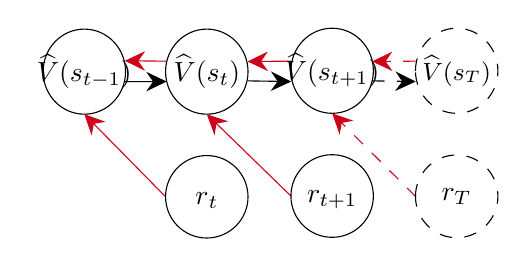
\begin{tikzpicture}[x=0.75pt,y=0.75pt,yscale=-1,xscale=1]
        
        %Straight Lines [id:da2592063600931961] 
        \draw [color={rgb, 255:red, 208; green, 2; blue, 27 }  ,draw opacity=1 ]   (282.5,135.16) -- (300.67,135.02) ;
        \draw [shift={(279.5,135.18)}, rotate = 359.55] [fill={rgb, 255:red, 208; green, 2; blue, 27 }  ,fill opacity=1 ][line width=0.08]  [draw opacity=0] (9.82,-4.72) -- (0,0) -- (9.82,4.72) -- (6.52,0) -- cycle    ;
        %Straight Lines [id:da41585806917853485] 
        \draw [color={rgb, 255:red, 208; green, 2; blue, 27 }  ,draw opacity=1 ]   (223.33,134.87) -- (240.67,135.02) ;
        \draw [shift={(220.33,134.85)}, rotate = 0.47] [fill={rgb, 255:red, 208; green, 2; blue, 27 }  ,fill opacity=1 ][line width=0.08]  [draw opacity=0] (9.82,-4.72) -- (0,0) -- (9.82,4.72) -- (6.52,0) -- cycle    ;
        %Shape: Ellipse [id:dp31493856088290983] 
        \draw   (181,140.07) .. controls (181,128.75) and (189.89,119.58) .. (200.86,119.58) .. controls (211.83,119.58) and (220.72,128.75) .. (220.72,140.07) .. controls (220.72,151.4) and (211.83,160.57) .. (200.86,160.57) .. controls (189.89,160.57) and (181,151.4) .. (181,140.07) -- cycle ;
        %Shape: Ellipse [id:dp5103941395609547] 
        \draw  [dash pattern={on 4.5pt off 4.5pt}] (360.4,139.66) .. controls (360.4,128.34) and (369.29,119.16) .. (380.26,119.16) .. controls (391.23,119.16) and (400.12,128.34) .. (400.12,139.66) .. controls (400.12,150.98) and (391.23,160.16) .. (380.26,160.16) .. controls (369.29,160.16) and (360.4,150.98) .. (360.4,139.66) -- cycle ;
        %Straight Lines [id:da30559831832260953] 
        \draw [color={rgb, 255:red, 0; green, 0; blue, 0 }  ,draw opacity=1 ]   (220.07,144.9) -- (237.5,144.86) ;
        \draw [shift={(240.5,144.85)}, rotate = 539.86] [fill={rgb, 255:red, 0; green, 0; blue, 0 }  ,fill opacity=1 ][line width=0.08]  [draw opacity=0] (9.82,-4.72) -- (0,0) -- (9.82,4.72) -- (6.52,0) -- cycle    ;
        %Shape: Ellipse [id:dp12377292733336898] 
        \draw  [color={rgb, 255:red, 0; green, 0; blue, 0 }  ,draw opacity=1 ] (240,140.07) .. controls (240,128.75) and (248.89,119.58) .. (259.86,119.58) .. controls (270.83,119.58) and (279.72,128.75) .. (279.72,140.07) .. controls (279.72,151.4) and (270.83,160.57) .. (259.86,160.57) .. controls (248.89,160.57) and (240,151.4) .. (240,140.07) -- cycle ;
        %Shape: Ellipse [id:dp9248757796917767] 
        \draw   (300.4,139.66) .. controls (300.4,128.34) and (309.29,119.16) .. (320.26,119.16) .. controls (331.23,119.16) and (340.12,128.34) .. (340.12,139.66) .. controls (340.12,150.98) and (331.23,160.16) .. (320.26,160.16) .. controls (309.29,160.16) and (300.4,150.98) .. (300.4,139.66) -- cycle ;
        %Straight Lines [id:da050274800713848156] 
        \draw [color={rgb, 255:red, 208; green, 2; blue, 27 }  ,draw opacity=1 ]   (202.96,162.71) -- (240,200.37) ;
        \draw [shift={(200.86,160.57)}, rotate = 45.48] [fill={rgb, 255:red, 208; green, 2; blue, 27 }  ,fill opacity=1 ][line width=0.08]  [draw opacity=0] (9.82,-4.72) -- (0,0) -- (9.82,4.72) -- (6.52,0) -- cycle    ;
        %Straight Lines [id:da7059353635730191] 
        \draw [color={rgb, 255:red, 208; green, 2; blue, 27 }  ,draw opacity=1 ]   (262.01,162.66) -- (300.4,200) ;
        \draw [shift={(259.86,160.57)}, rotate = 44.2] [fill={rgb, 255:red, 208; green, 2; blue, 27 }  ,fill opacity=1 ][line width=0.08]  [draw opacity=0] (9.82,-4.72) -- (0,0) -- (9.82,4.72) -- (6.52,0) -- cycle    ;
        %Straight Lines [id:da17885982011746426] 
        \draw [color={rgb, 255:red, 208; green, 2; blue, 27 }  ,draw opacity=1 ] [dash pattern={on 4.5pt off 4.5pt}]  (322.38,162.28) -- (360.4,200.16) ;
        \draw [shift={(320.26,160.16)}, rotate = 44.9] [fill={rgb, 255:red, 208; green, 2; blue, 27 }  ,fill opacity=1 ][line width=0.08]  [draw opacity=0] (9.82,-4.72) -- (0,0) -- (9.82,4.72) -- (6.52,0) -- cycle    ;
        %Shape: Ellipse [id:dp3523005799699832] 
        \draw  [dash pattern={on 4.5pt off 4.5pt}] (360.4,200.16) .. controls (360.4,189.16) and (369.29,180.23) .. (380.26,180.23) .. controls (391.23,180.23) and (400.12,189.16) .. (400.12,200.16) .. controls (400.12,211.17) and (391.23,220.09) .. (380.26,220.09) .. controls (369.29,220.09) and (360.4,211.17) .. (360.4,200.16) -- cycle ;
        %Shape: Ellipse [id:dp3509500153089894] 
        \draw   (300.4,200) .. controls (300.4,189) and (309.29,180.09) .. (320.26,180.09) .. controls (331.23,180.09) and (340.12,189) .. (340.12,200) .. controls (340.12,210.99) and (331.23,219.9) .. (320.26,219.9) .. controls (309.29,219.9) and (300.4,210.99) .. (300.4,200) -- cycle ;
        %Shape: Ellipse [id:dp17336392317383575] 
        \draw  [color={rgb, 255:red, 0; green, 0; blue, 0 }  ,draw opacity=1 ] (240,200.37) .. controls (240,189.4) and (248.89,180.5) .. (259.86,180.5) .. controls (270.83,180.5) and (279.72,189.4) .. (279.72,200.37) .. controls (279.72,211.34) and (270.83,220.23) .. (259.86,220.23) .. controls (248.89,220.23) and (240,211.34) .. (240,200.37) -- cycle ;
        %Straight Lines [id:da21459790152477998] 
        \draw [color={rgb, 255:red, 0; green, 0; blue, 0 }  ,draw opacity=1 ]   (279.5,144.52) -- (297.5,144.8) ;
        \draw [shift={(300.5,144.85)}, rotate = 180.91] [fill={rgb, 255:red, 0; green, 0; blue, 0 }  ,fill opacity=1 ][line width=0.08]  [draw opacity=0] (9.82,-4.72) -- (0,0) -- (9.82,4.72) -- (6.52,0) -- cycle    ;
        %Straight Lines [id:da8588950475203374] 
        \draw [color={rgb, 255:red, 208; green, 2; blue, 27 }  ,draw opacity=1 ] [dash pattern={on 4.5pt off 4.5pt}]  (342.5,135.16) -- (360.67,135.02) ;
        \draw [shift={(339.5,135.18)}, rotate = 359.55] [fill={rgb, 255:red, 208; green, 2; blue, 27 }  ,fill opacity=1 ][line width=0.08]  [draw opacity=0] (9.82,-4.72) -- (0,0) -- (9.82,4.72) -- (6.52,0) -- cycle    ;
        %Straight Lines [id:da9169375689094925] 
        \draw [color={rgb, 255:red, 0; green, 0; blue, 0 }  ,draw opacity=1 ] [dash pattern={on 4.5pt off 4.5pt}]  (339.5,144.52) -- (357.5,144.8) ;
        \draw [shift={(360.5,144.85)}, rotate = 180.91] [fill={rgb, 255:red, 0; green, 0; blue, 0 }  ,fill opacity=1 ][line width=0.08]  [draw opacity=0] (9.82,-4.72) -- (0,0) -- (9.82,4.72) -- (6.52,0) -- cycle    ;
        
        % Text Node
        \draw (320.26,201.59) node    {$r_{t+1}$};
        % Text Node
        \draw (200.86,140.07) node    {$\widehat{V}(s_{t-1})$};
        % Text Node
        \draw (320.26,139.66) node    {$\widehat{V}(s_{t+1})$};
        % Text Node
        \draw (380.26,139.66) node  [font=\small]  {$\widehat{V}(s_{T})$};
        % Text Node
        \draw (259.86,202) node  [color={rgb, 255:red, 208; green, 9; blue, 2 }  ,opacity=1 ]  {$\textcolor[rgb]{0,0,0}{r}\textcolor[rgb]{0,0,0}{_{t}}$};
        % Text Node
        \draw (259.86,140.07) node  [color={rgb, 255:red, 208; green, 9; blue, 2 }  ,opacity=1 ]  {$\textcolor[rgb]{0,0,0}{\widehat{V}}\textcolor[rgb]{0,0,0}{(s_{t})}$};
        % Text Node
        \draw (380.26,200.16) node    {$r_{T}$};

        \end{tikzpicture}
    \end{adjustbox}
  \end{center}
\caption{\textbf{Graphical representation of TD Learning}. Red arrows indicate the flow of the computations for deriving $\delta$ and updating $\widehat{V}$ expressed by equations \ref{td_error} and \ref{td_update}. Black arrows instead indicate the changes of $\widehat{V}$ moving from $s$ to $s_{t+1}$. Solid circles indicate states which have already been observed while dashed ones represent future not-yet observed states.}
\label{fig: td_learning}
\end{figure}
McClure \textit{et. al.} proposed that incentive salience is represented by $V$ as defined in equation \ref{td_v} while the error signal expressed by equation \ref{td_error} represents the activity of dopaminergic neurons with the dual function of driving the attribution of incentive salience (through reward prediction error coding as specified in section \ref{incentive_salience}) and guiding the previously mentioned action selection process \cite{schultz1997neural,mcclure2003computational,o2003temporal}. However, in later work, Zhang \textit{et. al.} highlighted the fact that the model proposed by McClure \textit{et. al.} fails to take into account an important part of the original incentive salience hypothesis: the dynamic modulation produced by the individual's internal state (see section \ref{wanting}) \cite{toates1994comparing,mcclure2003computational,berridge2004motivation,zhang2009neural,tindell2009dynamic,berridge2012prediction}. Zhang \textit{et. al.} therefore proposed a modification of the original TD Learning model to include a modulatory factor $k \in [0, +\infty]$ which can enhance ($k > 1$), dampen or even revert ($k < 1$) previously learned incentive salience values
\begin{align}
    \label{zhang_td_v}
    V(s_t) = \mathbb{E}[\tilde{r}(r_{t+1},k_{t}) + \gamma V(s_{t+1})]
\end{align}
here $\tilde{r}(.,.)$ is a function of two variables and can assume either an additive or multiplicative form \footnote{See \cite{zhang2009neural} for detailed description of the two forms and their functional differences.}. The main difference between the approaches of McClure \textit{et. al.} and Zhang \textit{et. al.} lies in the interpretation of $V$. Both authors see it as a combination of cached value (i.e. what has been learned from past experiences) and expectation over future $r$ but for McClure \textit{et. al.} all the future $r$ have the same weight while for Zhang \textit{et. al.} the state of the individual dynamically modulates the weighting of $r$. Using the notation from section \ref{incentive_salience}, we can say that the interaction $s$ between $I$ and $O$ at time $t_{+1}$ arises from the $V$ (i.e. incentive salience) generated after $s_{t}$. The mismatch between the predicted amount of reward and the actual reward received at time $t_{+1}$ generates an error signal that allows $I$ to learn about the "correct" magnitude of $V(s_{t})$ \cite{schultz2017reward} . As an example, an individual may anticipate that eating their favourite meal would be a rewarding experience but instead (for some reason) it was underwhelming. They therefore reduce the salience previously attributed to it. Importantly, $V(s_{t})$ does not just encompass the previous history of interactions between an individual and an object but also the current state of the individual themselves: the individual has learned from long experience that eating is a pleasurable activity but currently, since they are sated they do not expect much reward from doing it again in the near future.  \\
\\
In this view, motivation can be described as a mechanism that guides the interaction between individuals and objects. It controls and selects behaviours which are expected to lead to pleasurable outcomes for the individual (i.e. incentives or reward). These expectancies are the product of a learning process that can be modulated by the internal state of the individual. Therefore, from a behavioural point of view, an objects $O$ can acquire salience for an individual $I$ conditioned on its capacity to elicit rewarding experience $r$ \cite{berridge1998role,mcclure2003computational}. The amount of attributed salience is a valued representation of $O$ generated by $I$ and controls how likely and intense future interactions between the two will be. \cite{berridge1998role,mcclure2003computational}. Let $B$ represents the strength of an interaction between $I$ and $O$, $r$ a measure of how rewarding the interaction with $O$ is perceived to be and $V$ the generated attributed incentive salience.
\begin{figure}[h]
  \begin{center}
    \begin{adjustbox}{width=0.5\columnwidth}

        \tikzset{every picture/.style={line width=0.75pt}}
        
        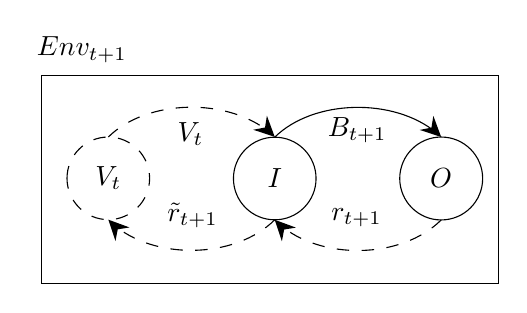
\begin{tikzpicture}[x=0.75pt,y=0.75pt,yscale=-1,xscale=1]
        
        %Shape: Circle [id:dp8739177923629333] 
        \draw   (123.48,130.05) .. controls (123.48,119.06) and (132.39,110.15) .. (143.38,110.15) .. controls (154.37,110.15) and (163.28,119.06) .. (163.28,130.05) .. controls (163.28,141.04) and (154.37,149.95) .. (143.38,149.95) .. controls (132.39,149.95) and (123.48,141.04) .. (123.48,130.05) -- cycle ;
        %Curve Lines [id:da2726669379173874] 
        \draw    (143.38,110.15) .. controls (161.99,91.83) and (200.82,90.88) .. (221.41,108.12) ;
        \draw [shift={(223.57,110.07)}, rotate = 224.02] [fill={rgb, 255:red, 0; green, 0; blue, 0 }  ][line width=0.08]  [draw opacity=0] (9.82,-4.72) -- (0,0) -- (9.82,4.72) -- (6.52,0) -- cycle    ;
        %Curve Lines [id:da4485667818478689] 
        \draw  [dash pattern={on 4.5pt off 4.5pt}]  (223.57,150.02) .. controls (204.36,169.14) and (165.2,169.5) .. (145.45,151.93) ;
        \draw [shift={(143.38,149.95)}, rotate = 405.89] [fill={rgb, 255:red, 0; green, 0; blue, 0 }  ][line width=0.08]  [draw opacity=0] (9.82,-4.72) -- (0,0) -- (9.82,4.72) -- (6.52,0) -- cycle    ;
        %Shape: Circle [id:dp8060688469385651] 
        \draw   (203.6,130.05) .. controls (203.6,119.01) and (212.54,110.07) .. (223.57,110.07) .. controls (234.6,110.07) and (243.55,119.01) .. (243.55,130.05) .. controls (243.55,141.08) and (234.6,150.02) .. (223.57,150.02) .. controls (212.54,150.02) and (203.6,141.08) .. (203.6,130.05) -- cycle ;
        %Shape: Rectangle [id:dp6054697635081123] 
        \draw   (31.2,80.5) -- (251.2,80.5) -- (251.2,180.83) -- (31.2,180.83) -- cycle ;
        %Shape: Circle [id:dp6091430023771998] 
        \draw  [dash pattern={on 4.5pt off 4.5pt}] (43.29,129.97) .. controls (43.29,118.98) and (52.2,110.07) .. (63.19,110.07) .. controls (74.18,110.07) and (83.09,118.98) .. (83.09,129.97) .. controls (83.09,140.96) and (74.18,149.87) .. (63.19,149.87) .. controls (52.2,149.87) and (43.29,140.96) .. (43.29,129.97) -- cycle ;
        %Curve Lines [id:da9876749075069771] 
        \draw  [dash pattern={on 4.5pt off 4.5pt}]  (143.38,149.95) .. controls (124.17,169.06) and (85.01,169.42) .. (65.26,151.85) ;
        \draw [shift={(63.19,149.87)}, rotate = 405.89] [fill={rgb, 255:red, 0; green, 0; blue, 0 }  ][line width=0.08]  [draw opacity=0] (9.82,-4.72) -- (0,0) -- (9.82,4.72) -- (6.52,0) -- cycle    ;
        %Curve Lines [id:da9412329086480583] 
        \draw  [dash pattern={on 4.5pt off 4.5pt}]  (63.19,110.07) .. controls (81.8,91.76) and (120.63,90.8) .. (141.21,108.05) ;
        \draw [shift={(143.38,110)}, rotate = 224.02] [fill={rgb, 255:red, 0; green, 0; blue, 0 }  ][line width=0.08]  [draw opacity=0] (9.82,-4.72) -- (0,0) -- (9.82,4.72) -- (6.52,0) -- cycle    ;
        
        % Text Node
        \draw (143.38,130.05) node  [font=\normalsize]  {$I$};
        % Text Node
        \draw (223.57,130.05) node  [font=\normalsize]  {$O$};
        % Text Node
        \draw (183.14,106.95) node  [font=\normalsize]  {$B_{t+1}$};
        % Text Node
        \draw (182.81,148.81) node  [font=\normalsize]  {$r_{t+1}$};
        % Text Node
        \draw (50.45,68.01) node  [font=\normalsize,rotate=-0.16]  {$Env_{t+1}$};
        % Text Node
        \draw (63.19,129.97) node  [font=\normalsize]  {$V_{t}$};
        % Text Node
        \draw (103.81,147.81) node  [font=\normalsize]  {$\tilde{r}_{t+1}$};
        % Text Node
        \draw (102.81,108.81) node  [font=\normalsize]  {$V_{t}$};
        \end{tikzpicture}
    \end{adjustbox}
  \end{center}
\caption[\textbf{The process of incentive salience attribution}]{Solid and dashed elements represent respectively observable (i.e. behavioural) and latent aspects of the process. The individual and the object that they interact with are indicated by $I$ and $O$. The strength of the interaction is represented by $B$. The salience that $I$ attributes to $O$ is expressed by $V$ while $r$ and $\tilde{r}$ are the experienced reward and its weighted version produced by the state of $I$. All the contextual factors influencing both the amount of $r$ perceived and the magnitude of $B$ produced are represented by $Env$. The dynamical natures of the process is expressed though the arbitrary temporal unit $t$.}
\label{fig: incs}
\end{figure}
Following Figure \ref{fig: incs}, at time $t+1$ an individual will produce an interaction with an object of strength $B$ according to the previous $V_{t}$. If we recall from section \ref{learning}, this process relies heavily on learning mechanisms making $V$ by nature dynamic and mutable. It should be noted that $B$ can be represented as a multidimensional variable defined by the instrumental behaviours conventionally used for assessing the \emph{wanting} component in animal studies (e.g. frequency, amount and duration of feeding behaviours like bites, nibbles and sniffs) \cite{berridge1998role}. During and after the interaction $I$ will experience a variable degree of reward $r_{t+1}$ that, weighted by their internal state, will then be used for updating $V_{t}$.  It is worth noting that the individual's internal state is not the only factor involved in the modulation of $r$, also the context in which $I$ and $O$ interact ($Env_{t+1}$ in Figure \ref{fig: incs}) seems to contribute to this \cite{palminteri2015contextual}. Following the idea presented in section \ref{manifold_rep_incentive_salience}, the latent state defined by $V$ could be represented as a manifold defined by the activity of those regions responsible for the attribution of incentive salience. Moreover, given the strong coupling between attributed incentive salience and behaviour \cite{berridge1998role} we would also expect the structure of this manifold to be a suitable descriptor of the behavioural aspects of attributed incentive salience.

\paragraph*{\textbf{From TD to Supervised Learning}}
\label{td_to_supervised}The approaches discussed above frame the estimation of attributed incentive salience as a reinforcement learning task. This requires the simulation of a sequence of interactions between $I$ and $O$ and the concomitant delivery of $r$  \cite{schultz1997neural,mcclure2003computational,zhang2009neural}. However, it is not always straightforward to replicate these interactions in real world scenarios, especially when dealing with human participants. The control on the internal state of $I$ and amount of $r$ delivered that McClure and Zhang assume is usually based on strict assumptions and can be achieved only in controlled experimental settings \cite{mcclure2003computational,zhang2009neural}. As an alternative solution for inferring $V$ outside the laboratory we propose to learn its manifold structure through supervised learning. Differently to what reported in the literature \cite{calhoun2019unsupervised, mccullough2021unsupervised, luxem2020identifying, pereira2020quantifying, shi2021learning} we argue that in this case the use of supervised in place of un-supervised techniques is to be preferred. Indeed, since we are dealing exclusively with behavioural data and trying to solve an inverse problem  we would like to learn a manifold structure which is not just a generic indicator of behavioural phenotype \cite{luxem2020identifying} but also obeys to specific functional constrains.\\
\\
In this approach, an experimenter gathers data on a set of interactions between $I$ and $O$ and let a learning algorithm to estimate two functions:
\begin{gather}
\label{supervised_v}
    V(s_{t}) = f^{1}(O, \tilde{r_{t}}, V(s_{t-1}); \theta^{1}) \\
    r_{t+1} = f^{2}(V(s_{t}); \theta^{2}) \nonumber
\end{gather}
here $f^{1}$ and $f^{2}$ are arbitrarily complex functions while $\theta^{1}$ and $\theta^{2}$ are parameters that the learning algorithm has to infer. The future reward that an individual expects after an interaction with an object is produced by the current level of attributed salience, which  itself is a function of the current internal state of the individual (expressed through the amount of reward just experienced) and the incentive salience previously attributed to the object. It is important to note that the two functions above need to be recursive over all $s \in S$ (see equations \ref{td_v} and \ref{zhang_td_v}) in order to provide $V(s_{t})$ with the dual purpose of caching all the past $V$ and being a suitable predictor for all the $r$. This formulation however still requires a measure of the $r$ experienced by $I$ (or more precisely its weighted version $\tilde{r}$) after interacting with $O$, which is not easily accessible. However, Thorndike's law of effect \cite{thorndike1927law} and Skinner's operant conditioning principles \cite{skinner1965science} suggest that $r$, which  like $V$ is a non observable latent variable, manifests itself through the intensity of interactions between $I$ and $O$ (i.e. $B$ in Figure \ref{fig: incs}): the frequency and amount of object-directed behaviours increase or decrease as a function of the rewards an individual expects to receive \cite{berridge2004motivation,schultz2017reward}. Since $V(s_{t})$ predicts how much $r$ an $I$ expects to receive from interacting with $O$, we should also expect the strength of their future interactions to be a function of $V(s_{t})$. This can be represented re-arranging the equations in \ref{supervised_v} in a more compact form as a chain of functions
\begin{align}
\label{supervised_b}
    B_{t+1} = f^{2}(f^{1}(O, B_{t}, V(s_{t-1}); \theta^{1});  \theta^{2})
\end{align}
To approximate the above expression, a learning algorithm would require records of behaviours generated by individuals while interacting with a diverse set of potentially rewarding objects. Here, we argue that video games are one way to obtain this type of data at scale while also achieving some level of ecological validity.

\subsection{Video Games and Telemetry}
\label{videogame_telemetries}
As we highlighted in chapter \ref{chapter_lit_review}, interacting with video games is a volitional activity driven largely by the capacity of the games to provide pleasurable experiences \cite{boyle2012engagement}. Behaviour within the game is best understood as the result of a value attribution process similar to that of secondary reward objects (see section \ref{incentive_salience}). Indeed, it appears that the play behaviour is often produced and maintained by the structural characteristics of the game (e.g. game mechanics) \cite{king2010video} which, working like conventional reinforcement mechanisms \cite{chumbley2006affect,wang2011game,phillips2013videogame,avserivskis2017computational}, produce effects similar to operant conditioning \cite{skinner1965science}. Although caution should be applied when complex activities are investigated using neuroimaging techniques, evidence suggest that the maintenance of video games playing behaviour engages the same cortico-striatal structures \cite{hoeft2008gender,mathiak2011reward,cole2012interactivity,klasen2012neural,lorenz2015video,gleich2017functional} and neurotransmitters \cite{koepp1998evidence} involved in reward processing. This, seems also supported at the behavioural level where the ammount of experienced in-game reward appears to play a role in controlling how likely is an individual to keep engaging in playing behaviour \cite{agarwal2017quitting, steyvers2019joint}. This, in conjunction with a growing literature highlighting similarities between certain video game mechanics and activities driven by secondary rewards (e.g. gambling) \cite{king2010role,drummond2018video,zendle2018video}, corroborates the idea that video games are able to elicit behavioural responses through incentive mechanics. In this view, video games with different structural characteristics could be seen as objects possessing rewarding properties that heavily depend on the individuals interacting with them (e.g. an individual's preference for a specific game mechanic). Hence, similarly to the process specified in chapter \ref{chapter_lit_review}, we can expect that through repeated interactions, an individual will experience varying degrees of reward determined by their internal state and the characteristics of the game. These interactions will produce continuous adjustments in the level of saliency attributed to playing that specific game which in turn will influence the frequency and amount of future interactions with that same game. Other than offering a context for observing the process of incentive salience attribution, video games allow us to obtain large volumes of behavioural data (similar to those mentioned in chapter \ref{chapter_lit_review}) in a naturalistic fashion. This is made possible by the widespread practice of obtaining high frequency records (i.e. telemetry\footnote{See \cite{el2016game} for a more technical description of telemetry in video games.}) of players' behaviour during the game \cite{drachen2015behavioral}. This approach, despite offering less control and rigour than conventional experimental procedures, allows us to obtain a more faithful representation of natural behaviour (similarly to field studies) while avoiding some of the limitations connected with laboratory-based studies (e.g. sampling and observer biases).
\newline
\newline
In order to use this type of behavioural data to model attributed incentive salience, a learning algorithm should possess the following properties. First, it should be scalable and noise resilient, to leverage large volumes of naturalistic data in an efficient and effective manner. Second, it should be able to approximate arbitrarily complex functions, given that the shape of the functions specified in equation \ref{td_to_supervised} is not known a-priori. And finally, it should be able to produce an approximation of $V(s_{t})$ that can be inspected in order to evaluate if its functional properties can be compared with those of attributed incentive salience. Artificial Neural Networks (ANNs) appear to satisfy these requirements.

\subsection{Artificial Neural Networks}
\label{artificial_neural_networks}
In their conventional form, ANNs can be seen as chains of nested functions (the layers of the network). These layers are vector valued (there are multiple units or neurons in each layer) and organized as directed acyclic computational graphs (information only flows forward). When the number of layers is greater than two, the prefix "deep" is usually applied \cite{bengio2017deep}. The goal of this ensemble of functions is to create a mapping between an input $x$ and a target $y$. Following the example illustrated in Figure \ref{fig: ffnn}, given the set of parameters $\Theta = \{\theta^1, \theta^2 \}$ an ANN would first infer a function $h = f(x;\theta^{1})$, mapping the input to a new representation $h$. The same representation $h$ would then become the input of a second function $\widehat{y} = f^{1}(h;\theta^{2})$ which produces an estimate of the target \cite{bengio2017deep}. In this sense, we can think of each layer as a collection of many non-linear vector to scalar functions taking the previous layer as input and generating the units for the layer that follows \cite{bengio2017deep}. By increasing the number of layers and units, ANNs can approximate an extremely large class of functions \cite{rumelhart1986learning}.
\begin{figure}
    \begin{center}
        \begin{adjustbox}{width=0.4\textwidth}
            \tikzset{every picture/.style={line width=0.75pt}} %set default line width to 0.75pt        
            
            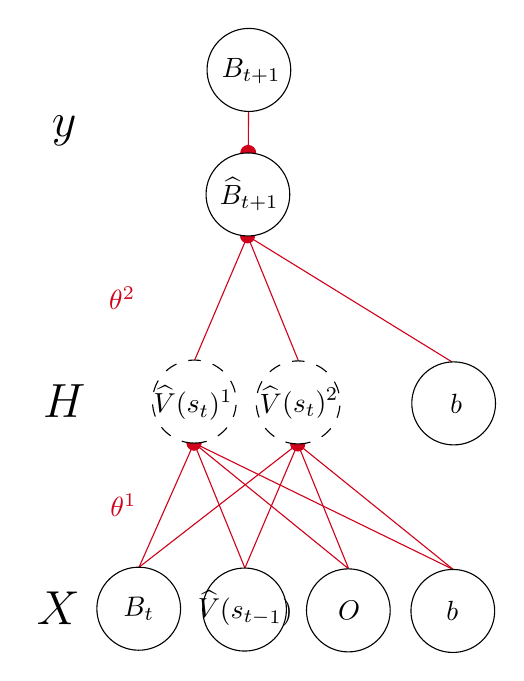
\begin{tikzpicture}[x=0.75pt,y=0.75pt,yscale=-1,xscale=1]
            %uncomment if require: \path (0,350); %set diagram left start at 0, and has height of 350
            
            %Straight Lines [id:da8866607252953388] 
            \draw [color={rgb, 255:red, 208; green, 2; blue, 27 }  ,draw opacity=1 ]   (227.88,279.44) -- (254.36,219.65) ;
            \draw [shift={(254.36,219.65)}, rotate = 293.89] [color={rgb, 255:red, 208; green, 2; blue, 27 }  ,draw opacity=1 ][fill={rgb, 255:red, 208; green, 2; blue, 27 }  ,fill opacity=1 ][line width=0.75]      (0, 0) circle [x radius= 3.02, y radius= 3.02]   ;
            %Straight Lines [id:da0731191645042184] 
            \draw [color={rgb, 255:red, 208; green, 2; blue, 27 }  ,draw opacity=1 ]   (254.68,179.65) -- (280.16,119.85) ;
            \draw [shift={(280.16,119.85)}, rotate = 293.08] [color={rgb, 255:red, 208; green, 2; blue, 27 }  ,draw opacity=1 ][fill={rgb, 255:red, 208; green, 2; blue, 27 }  ,fill opacity=1 ][line width=0.75]      (0, 0) circle [x radius= 3.02, y radius= 3.02]   ;
            %Straight Lines [id:da4826752085294559] 
            \draw [color={rgb, 255:red, 208; green, 2; blue, 27 }  ,draw opacity=1 ]   (304.68,180.05) -- (280.16,119.85) ;
            \draw [shift={(280.16,119.85)}, rotate = 247.84] [color={rgb, 255:red, 208; green, 2; blue, 27 }  ,draw opacity=1 ][fill={rgb, 255:red, 208; green, 2; blue, 27 }  ,fill opacity=1 ][line width=0.75]      (0, 0) circle [x radius= 2.01, y radius= 2.01]   ;
            %Straight Lines [id:da39539248901414714] 
            \draw [color={rgb, 255:red, 208; green, 2; blue, 27 }  ,draw opacity=1 ]   (328.88,280.25) -- (304.36,220.05) ;
            \draw [shift={(304.36,220.05)}, rotate = 247.84] [color={rgb, 255:red, 208; green, 2; blue, 27 }  ,draw opacity=1 ][fill={rgb, 255:red, 208; green, 2; blue, 27 }  ,fill opacity=1 ][line width=0.75]      (0, 0) circle [x radius= 3.02, y radius= 3.02]   ;
            %Straight Lines [id:da8990891706173756] 
            \draw [color={rgb, 255:red, 208; green, 2; blue, 27 }  ,draw opacity=1 ]   (278.88,279.85) -- (254.36,219.65) ;
            \draw [shift={(254.36,219.65)}, rotate = 247.84] [color={rgb, 255:red, 208; green, 2; blue, 27 }  ,draw opacity=1 ][fill={rgb, 255:red, 208; green, 2; blue, 27 }  ,fill opacity=1 ][line width=0.75]      (0, 0) circle [x radius= 3.02, y radius= 3.02]   ;
            %Straight Lines [id:da1147021220204143] 
            \draw [color={rgb, 255:red, 208; green, 2; blue, 27 }  ,draw opacity=1 ]   (328.88,280.25) -- (254.36,219.65) ;
            \draw [shift={(254.36,219.65)}, rotate = 219.12] [color={rgb, 255:red, 208; green, 2; blue, 27 }  ,draw opacity=1 ][fill={rgb, 255:red, 208; green, 2; blue, 27 }  ,fill opacity=1 ][line width=0.75]      (0, 0) circle [x radius= 3.02, y radius= 3.02]   ;
            %Straight Lines [id:da30405558125224674] 
            \draw [color={rgb, 255:red, 208; green, 2; blue, 27 }  ,draw opacity=1 ]   (278.88,279.85) -- (304.36,220.05) ;
            \draw [shift={(304.36,220.05)}, rotate = 293.08] [color={rgb, 255:red, 208; green, 2; blue, 27 }  ,draw opacity=1 ][fill={rgb, 255:red, 208; green, 2; blue, 27 }  ,fill opacity=1 ][line width=0.75]      (0, 0) circle [x radius= 3.02, y radius= 3.02]   ;
            %Straight Lines [id:da7841365763851936] 
            \draw [color={rgb, 255:red, 208; green, 2; blue, 27 }  ,draw opacity=1 ]   (227.88,279.44) -- (304.36,220.05) ;
            \draw [shift={(304.36,220.05)}, rotate = 322.17] [color={rgb, 255:red, 208; green, 2; blue, 27 }  ,draw opacity=1 ][fill={rgb, 255:red, 208; green, 2; blue, 27 }  ,fill opacity=1 ][line width=0.75]      (0, 0) circle [x radius= 3.02, y radius= 3.02]   ;
            %Straight Lines [id:da5618158283475858] 
            \draw [color={rgb, 255:red, 208; green, 2; blue, 27 }  ,draw opacity=1 ]   (379.21,280.52) -- (304.36,220.05) ;
            \draw [shift={(304.36,220.05)}, rotate = 218.93] [color={rgb, 255:red, 208; green, 2; blue, 27 }  ,draw opacity=1 ][fill={rgb, 255:red, 208; green, 2; blue, 27 }  ,fill opacity=1 ][line width=0.75]      (0, 0) circle [x radius= 3.02, y radius= 3.02]   ;
            %Straight Lines [id:da4509011415852858] 
            \draw [color={rgb, 255:red, 208; green, 2; blue, 27 }  ,draw opacity=1 ]   (378.61,180.51) -- (280.16,119.85) ;
            \draw [shift={(280.16,119.85)}, rotate = 211.64] [color={rgb, 255:red, 208; green, 2; blue, 27 }  ,draw opacity=1 ][fill={rgb, 255:red, 208; green, 2; blue, 27 }  ,fill opacity=1 ][line width=0.75]      (0, 0) circle [x radius= 3.02, y radius= 3.02]   ;
            %Straight Lines [id:da7242656967921071] 
            \draw [color={rgb, 255:red, 208; green, 2; blue, 27 }  ,draw opacity=1 ]   (379.21,280.52) -- (254.36,219.65) ;
            \draw [shift={(254.36,219.65)}, rotate = 205.99] [color={rgb, 255:red, 208; green, 2; blue, 27 }  ,draw opacity=1 ][fill={rgb, 255:red, 208; green, 2; blue, 27 }  ,fill opacity=1 ][line width=0.75]      (0, 0) circle [x radius= 3.02, y radius= 3.02]   ;
            %Shape: Ellipse [id:dp9097533963365589] 
            \draw  [fill={rgb, 255:red, 255; green, 255; blue, 255 }  ,fill opacity=1 ][dash pattern={on 4.5pt off 4.5pt}] (304.36,220.05) .. controls (293.22,219.96) and (284.26,210.94) .. (284.35,199.89) .. controls (284.44,188.84) and (293.54,179.96) .. (304.68,180.05) .. controls (315.82,180.14) and (324.77,189.17) .. (324.69,200.21) .. controls (324.6,211.26) and (315.5,220.14) .. (304.36,220.05) -- cycle ;
            %Shape: Ellipse [id:dp9467435778420286] 
            \draw  [fill={rgb, 255:red, 255; green, 255; blue, 255 }  ,fill opacity=1 ][dash pattern={on 4.5pt off 4.5pt}] (254.36,219.65) .. controls (243.22,219.56) and (234.27,210.53) .. (234.36,199.49) .. controls (234.44,188.44) and (243.54,179.56) .. (254.68,179.65) .. controls (265.82,179.74) and (274.78,188.77) .. (274.69,199.81) .. controls (274.6,210.86) and (265.5,219.74) .. (254.36,219.65) -- cycle ;
            %Shape: Ellipse [id:dp4514100854948462] 
            \draw  [fill={rgb, 255:red, 255; green, 255; blue, 255 }  ,fill opacity=1 ] (379.29,220.52) .. controls (368.15,220.43) and (359.2,211.4) .. (359.29,200.36) .. controls (359.37,189.31) and (368.47,180.43) .. (379.61,180.52) .. controls (390.75,180.61) and (399.71,189.64) .. (399.62,200.68) .. controls (399.53,211.73) and (390.43,220.61) .. (379.29,220.52) -- cycle ;
            %Shape: Ellipse [id:dp2836578028815524] 
            \draw  [fill={rgb, 255:red, 255; green, 255; blue, 255 }  ,fill opacity=1 ] (227.56,319.44) .. controls (216.42,319.35) and (207.46,310.32) .. (207.55,299.28) .. controls (207.64,288.23) and (216.74,279.35) .. (227.88,279.44) .. controls (239.02,279.53) and (247.97,288.56) .. (247.89,299.6) .. controls (247.8,310.65) and (238.7,319.53) .. (227.56,319.44) -- cycle ;
            %Shape: Ellipse [id:dp10987171532240936] 
            \draw  [fill={rgb, 255:red, 255; green, 255; blue, 255 }  ,fill opacity=1 ] (278.56,319.85) .. controls (267.42,319.76) and (258.46,310.73) .. (258.55,299.69) .. controls (258.64,288.64) and (267.74,279.76) .. (278.88,279.85) .. controls (290.02,279.94) and (298.97,288.96) .. (298.88,300.01) .. controls (298.79,311.06) and (289.69,319.94) .. (278.56,319.85) -- cycle ;
            %Shape: Ellipse [id:dp5734471221931936] 
            \draw  [fill={rgb, 255:red, 255; green, 255; blue, 255 }  ,fill opacity=1 ] (328.56,320.25) .. controls (317.42,320.16) and (308.46,311.13) .. (308.55,300.09) .. controls (308.64,289.04) and (317.74,280.16) .. (328.88,280.25) .. controls (340.01,280.34) and (348.97,289.37) .. (348.88,300.41) .. controls (348.79,311.46) and (339.69,320.34) .. (328.56,320.25) -- cycle ;
            %Shape: Ellipse [id:dp8405299754625457] 
            \draw  [fill={rgb, 255:red, 255; green, 255; blue, 255 }  ,fill opacity=1 ] (378.89,320.52) .. controls (367.75,320.43) and (358.79,311.4) .. (358.88,300.36) .. controls (358.97,289.31) and (368.07,280.43) .. (379.21,280.52) .. controls (390.35,280.61) and (399.3,289.64) .. (399.21,300.68) .. controls (399.13,311.73) and (390.03,320.61) .. (378.89,320.52) -- cycle ;
            %Straight Lines [id:da531681756338569] 
            \draw [color={rgb, 255:red, 208; green, 2; blue, 27 }  ,draw opacity=1 ]   (280.48,79.86) -- (280.64,59.86) ;
            \draw [shift={(280.48,79.86)}, rotate = 270.46] [color={rgb, 255:red, 208; green, 2; blue, 27 }  ,draw opacity=1 ][fill={rgb, 255:red, 208; green, 2; blue, 27 }  ,fill opacity=1 ][line width=0.75]      (0, 0) circle [x radius= 3.35, y radius= 3.35]   ;
            %Shape: Ellipse [id:dp7122318662628844] 
            \draw  [fill={rgb, 255:red, 255; green, 255; blue, 255 }  ,fill opacity=1 ] (280.64,59.86) .. controls (269.51,59.77) and (260.55,50.74) .. (260.64,39.69) .. controls (260.73,28.65) and (269.83,19.77) .. (280.97,19.86) .. controls (292.1,19.95) and (301.06,28.97) .. (300.97,40.02) .. controls (300.88,51.06) and (291.78,59.95) .. (280.64,59.86) -- cycle ;
            %Shape: Ellipse [id:dp8923679098088735] 
            \draw  [fill={rgb, 255:red, 255; green, 255; blue, 255 }  ,fill opacity=1 ] (280.16,119.85) .. controls (269.03,119.76) and (260.07,110.74) .. (260.16,99.69) .. controls (260.25,88.65) and (269.35,79.77) .. (280.48,79.86) .. controls (291.62,79.94) and (300.58,88.97) .. (300.49,100.02) .. controls (300.4,111.06) and (291.3,119.94) .. (280.16,119.85) -- cycle ;
            
            % Text Node
            \draw (279.05,299.33) node  [rotate=-0.94] [align=left] {$\displaystyle \widehat{V}(s_{t-1})$};
            % Text Node
            \draw (329.04,300.22) node  [rotate=-1.88] [align=left] {$\displaystyle O$};
            % Text Node
            \draw (378.8,300.47) node  [rotate=-359.63] [align=left] {$\displaystyle b$};
            % Text Node
            \draw (380.6,200.87) node  [rotate=-358.65] [align=left] {$\displaystyle b$};
            % Text Node
            \draw (253.92,200.36) node  [rotate=-0.88] [align=left] {$\displaystyle \widehat{V}(s_{t})^1$};
            % Text Node
            \draw (305.05,199.96) node  [rotate=-358.47] [align=left] {$\displaystyle \widehat{V}(s_{t})^2$};
            % Text Node
            \draw (280.95,99.59) node  [rotate=-359.67] [align=left] {$\displaystyle \widehat{B}_{t+1}$};
            % Text Node
            \draw (189,299.2) node  [font=\LARGE,rotate=-0.33]  {$X$};
            % Text Node
            \draw (191.8,199.22) node  [font=\LARGE,rotate=-359.71]  {$H$};
            % Text Node
            \draw (191.84,69.22) node  [font=\LARGE,rotate=-0.13]  {$y$};
            % Text Node
            \draw (220.4,249.43) node  [font=\normalsize,color={rgb, 255:red, 0; green, 0; blue, 0 }  ,opacity=1 ,rotate=-359.94]  {$\textcolor[rgb]{0.82,0.01,0.11}{\theta }\textcolor[rgb]{0.82,0.01,0.11}{^{1}}$};
            % Text Node
            \draw (219.7,149.93) node  [font=\normalsize,color={rgb, 255:red, 208; green, 2; blue, 27 }  ,opacity=1 ,rotate=-359.3]  {$\textcolor[rgb]{0.82,0.01,0.11}{\theta }\textcolor[rgb]{0.82,0.01,0.11}{^{2}}$};
            % Text Node
            \draw (227.72,299.44) node  [rotate=-358] [align=left] {$\displaystyle B_{t}$};
            % Text Node
            \draw (281.85,40.31) node  [rotate=-359.39] [align=left] {$\displaystyle B_{t+1}$};
            
            
            \end{tikzpicture}
        \end{adjustbox}
    \end{center}
\caption[\textbf{Feedforward ANN with a 2-units hidden layer}]{The figure represents how a feedforward ANN could be used for estimating $V(s_t)$ given a sequence of observed behaviors ($B$) produced while interacting with an object ($O$). Here $X$ and $H$ indicates the model's input and the inferred representation.  $y$ indicates both the target and the estimate produced by the model while $b$ is a bias term. The collection of all the red lines indicates the $\Theta$ that the ANN has to estimate while each line represents a single parameter $w$ or $b$. The circles are computational units (i.e. artificial neurons) whose outputs are given by $\phi(W_i^ \top X+ b )$. Here, $\phi$ is a non-linear function conventionally called activation, $W_i$ the weight matrix for the $i^{th}$ unit, $b$ the bias vector and $X$ the output from the previous layer.}
\label{fig: ffnn}
\end{figure}
An ANN finds the optimal values for $\Theta$ by taking forward and a backward passes through the computational graph. In the forward pass, information flows from the input $x$ to the estimate $\widehat{y}$ according to the operations specified in Figure \ref{fig: ffnn}. During the backward pass, the error between $\widehat{y}$ and the target is first computed
\begin{gather}
\label{loss}
    \mathcal{L} = l(y, \widehat{y})
\end{gather}
Here $l$ is a generic convex and differentiable function measuring the distance between $y$ and $\widehat{y}$. Then, the gradient of the error with respect to all the parameters is found and an update is performed taking steps of size $\alpha \in [0, 1]$ in the direction opposite to the gradient
\begin{gather}
\label{delta_rule}
    \Delta w^{j}_{i} = -\alpha\frac{\partial \mathcal{L}}{\partial w^{j}_{i}} \\
    w^{j}_{i} \leftarrow w^{j}_{i} + \Delta w^{j}_{i} \nonumber
\end{gather}
What we illustrated here is the application of the delta rule for updating the $i^{th}$ parameter of the $j^{th}$ layer through gradient descent \cite{widrow1960adaptive}. Deep feedforward ANNs rely on a generalization of this rule (i.e. backpropagation \cite{rumelhart1986learning}) for efficiently computing the gradient for all the parameters in the network.  
\\
\\
Returning to the supervised learning problem specified in section \ref{td_to_supervised}, a feedforward ANN approximates $V(s_{t})$ by mapping the inputs of equation \ref{supervised_b} to a candidate $\widehat{V}(s_{t})$ which is then used to generate an estimate $\widehat{B}_{t+1}$. Then, during the backward pass $\widehat{V}(s_{t})$ is adjusted based on the degree of mismatch between the estimation that it produced and the real value of $B_{t+1}$. It is of interest to note that there is a certain degree of overlap between how ANNs adjust their weights and the TD update illustrated in section \ref{td_learning}. Indeed, in single-step scenarios (i.e. predicting $s_{t+1}$ based on $s_{t}$ for each $s \in S$) the parameter changes produced by the two methods are the same \cite{sutton1988learning}. The major difference lies in the delivery of the update: TD learning performs it at every step while backpropagation-based algorithms must  wait until the end of the sequence in order to collate all the observed errors in a single term \cite{sutton1988learning}.

\paragraph*{\textbf{Recurrent Neural Networks}}
\label{rnn_theory}
Despite their universal function approximation properties \cite{hornik1989multilayer}, feedforward ANNs are not suitable for the type of recursive operations expressed in paragraph \ref{td_to_supervised} \cite{bengio2017deep}. As we can see from Figure \ref{fig: ffnn_rnn}A, given a sequence of inputs and targets, a conventional feedforward ANN would be limited to learning a temporally local function of the form
\begin{gather}
\label{td_ffnn}
    B_{t+1} = f^2(f^1(O, B_{t}; \theta^{1}); \theta^{2})
\end{gather}
Even when $\Theta$ are shared across time, the estimated $\widehat{V}(s_t)$ cannot incorporate information from past $\widehat{V}(s)$ nor guarantee predictive power for the future $B$. A solution to this problem is offered by ANNs with feedback connections like Recurrent Neural Networks (RNNs). These  are a class of ANNs that are able to efficiently process long sequences of data while also relaxing the requirements of conventional feedforward ANNs for fixed length inputs \cite{bengio2017deep}. Looking at Figure \ref{fig: ffnn_rnn}B, we see that for each $t \in T$ a RNN would compute $\widehat{V}(s_t)$ using both the input $OB_{t}$ and the previously estimated representation $\widehat{V}(s_{t-1})$. This, in combination with the recursive application of $\Theta$, allows the network to learn a function over the entire temporal sequence and to provide $\widehat{V}(s_t)$ with the desirable properties mentioned in section \ref{td_to_supervised}. The structure of $\Theta$ is more complex in RNNs than in feedforward ANNs \footnote{See \cite{bengio2017deep} for a description of the parameters' structure in RNNs.} and a detailed derivation of the underlying optimization process is outside the scope of the present work. Nevertheless, it is worth singling out how the recurrent nature of the computations underlying the generation of $\widehat{V}(s_t)$  makes RNNs suitable for approximating the function specified in section \ref{td_to_supervised}. \\
\\
Following Figure \ref{fig: ffnn_rnn}B, let $\widehat{V}(s_t)$ be the representation inferred by the model at time $t$ and its associated parameters. Optimal parameter values are found through the same update rule used in feedforward ANNs
\begin{gather}
\label{bptt_1}
    \widehat{V}(s_t) \leftarrow \widehat{V}(s_t) + -\alpha \frac{\partial \mathcal{L}}{\partial \widehat{V}(s_t)}
\end{gather}
however, since $\mathcal{L}$ can now only be observed at the end of a temporal sequence, computing $\frac{\partial \mathcal{L}}{\partial \widehat{V}(s_t)}$ requires us to take into account all the intermediate steps from $t$ to $T$. This is achieved applying the chain rule and propagating the error gradient backward in time \cite{bengio2017deep,lillicrap2019backpropagation}
\begin{gather}
\label{bptt_2}
    \frac{\partial \mathcal{L}}{\partial \widehat{V}(s_t)} = 
    \frac{\partial \mathcal{L}}{\partial \widehat{V}(s_{T})}
    \frac{\partial \widehat{V}(s_{T})}{\partial \widehat{V}(s_{T-1})}
    \dots
    \frac{\partial \widehat{V}(s_{T-n})}{\partial \widehat{V}(s_{t})}
\end{gather}
This implies that, similarly to TD update, the error flow forces $\widehat{V}(s_t)$ to retain information from $OB_t$ and $\widehat{V}(s_{t-1})$ in order to perform estimation of $B_{t+1}$ while still being useful for generating $\widehat{V}(s_{t+1})$ as we can see from Figure \ref{fig: ffnn_rnn}B. This process is made more efficient by an RNN variant called Long Short-Term Memory (LSTM) \cite{hochreiter1997long}, which, as well as improving the propagation of the error gradient, has specialized mechanisms for inferring, at each point in time, which portion of information should be kept or discarded in order to minimize $\mathcal{L}$ \cite{hochreiter1997long,bengio2017deep}.
\begin{figure}[h]
\begin{center}
\begin{adjustbox}{width=0.5\columnwidth}
    \tikzset{every picture/.style={line width=0.75pt}} %set default line width to 0.75pt        
    
    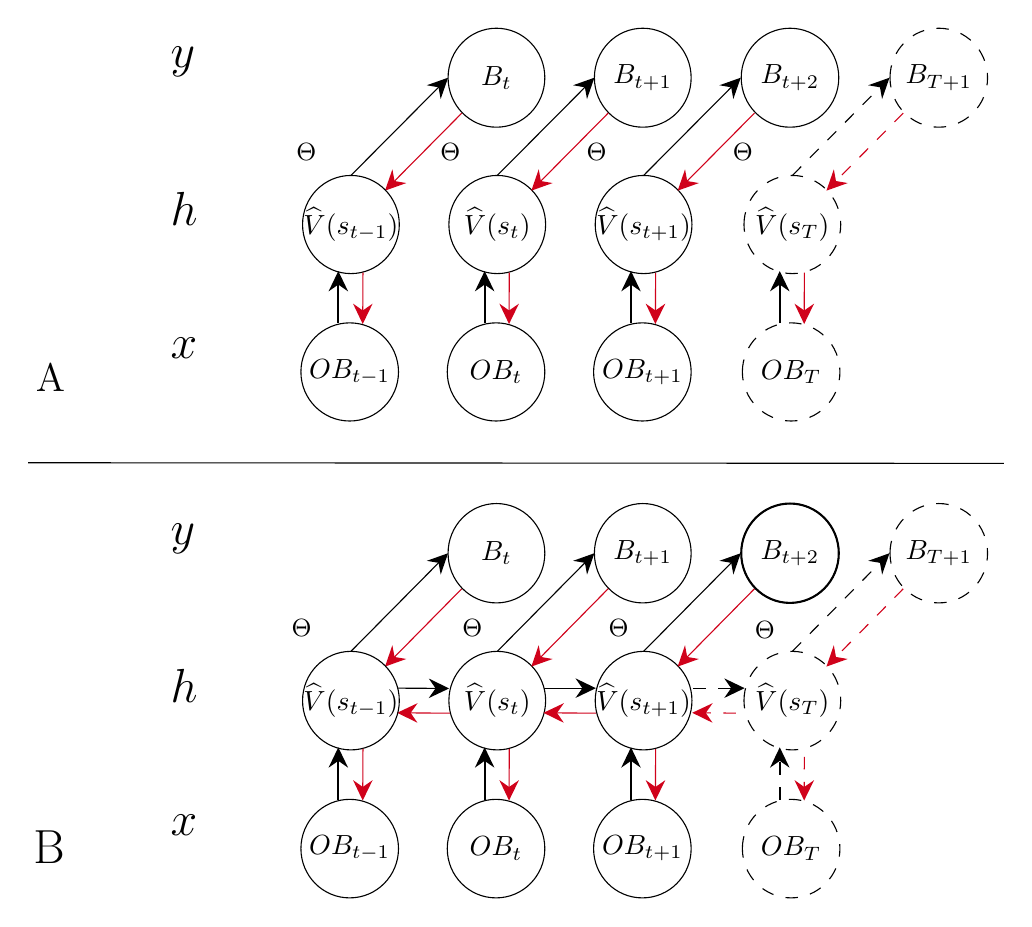
\begin{tikzpicture}[x=0.75pt,y=0.75pt,yscale=-1,xscale=1]
    %uncomment if require: \path (0,432); %set diagram left start at 0, and has height of 432
    
    %Shape: Ellipse [id:dp9152556376471453] 
    \draw   (252.87,325.26) .. controls (252.87,312.15) and (263.3,301.52) .. (276.18,301.52) .. controls (289.05,301.52) and (299.48,312.15) .. (299.48,325.26) .. controls (299.48,338.37) and (289.05,349) .. (276.18,349) .. controls (263.3,349) and (252.87,338.37) .. (252.87,325.26) -- cycle ;
    %Straight Lines [id:da0084456304461753] 
    \draw [color={rgb, 255:red, 208; green, 2; blue, 27 }  ,draw opacity=1 ]   (230.94,331.15) -- (253.32,331.31) ;
    \draw [shift={(227.94,331.12)}, rotate = 0.43] [fill={rgb, 255:red, 208; green, 2; blue, 27 }  ,fill opacity=1 ][line width=0.08]  [draw opacity=0] (9.82,-4.72) -- (0,0) -- (9.82,4.72) -- (6.52,0) -- cycle    ;
    %Shape: Ellipse [id:dp18326344407352502] 
    \draw   (181.58,396.56) .. controls (181.58,383.45) and (192.11,372.82) .. (205.08,372.82) .. controls (218.06,372.82) and (228.59,383.45) .. (228.59,396.56) .. controls (228.59,409.67) and (218.06,420.3) .. (205.08,420.3) .. controls (192.11,420.3) and (181.58,409.67) .. (181.58,396.56) -- cycle ;
    %Shape: Ellipse [id:dp4732045107682973] 
    \draw   (252.09,396.56) .. controls (252.09,383.45) and (262.61,372.82) .. (275.59,372.82) .. controls (288.57,372.82) and (299.09,383.45) .. (299.09,396.56) .. controls (299.09,409.67) and (288.57,420.3) .. (275.59,420.3) .. controls (262.61,420.3) and (252.09,409.67) .. (252.09,396.56) -- cycle ;
    %Straight Lines [id:da9106304988340169] 
    \draw    (205.67,301.52) -- (250.37,256.37) ;
    \draw [shift={(252.48,254.24)}, rotate = 494.71] [fill={rgb, 255:red, 0; green, 0; blue, 0 }  ][line width=0.08]  [draw opacity=0] (9.82,-4.72) -- (0,0) -- (9.82,4.72) -- (6.52,0) -- cycle    ;
    %Straight Lines [id:da5186602107869037] 
    \draw [color={rgb, 255:red, 208; green, 2; blue, 27 }  ,draw opacity=1 ]   (259.09,271.36) -- (224.2,306.73) ;
    \draw [shift={(222.1,308.86)}, rotate = 314.62] [fill={rgb, 255:red, 208; green, 2; blue, 27 }  ,fill opacity=1 ][line width=0.08]  [draw opacity=0] (9.82,-4.72) -- (0,0) -- (9.82,4.72) -- (6.52,0) -- cycle    ;
    %Shape: Ellipse [id:dp6434768624828036] 
    \draw   (322.59,396.56) .. controls (322.59,383.45) and (333.11,372.82) .. (346.09,372.82) .. controls (359.07,372.82) and (369.59,383.45) .. (369.59,396.56) .. controls (369.59,409.67) and (359.07,420.3) .. (346.09,420.3) .. controls (333.11,420.3) and (322.59,409.67) .. (322.59,396.56) -- cycle ;
    %Shape: Ellipse [id:dp4847846412537088] 
    \draw   (252.48,254.24) .. controls (252.48,241.02) and (262.91,230.3) .. (275.78,230.3) .. controls (288.65,230.3) and (299.09,241.02) .. (299.09,254.24) .. controls (299.09,267.46) and (288.65,278.18) .. (275.78,278.18) .. controls (262.91,278.18) and (252.48,267.46) .. (252.48,254.24) -- cycle ;
    %Shape: Ellipse [id:dp07973567399208026] 
    \draw   (322.98,254.24) .. controls (322.98,241.02) and (333.42,230.3) .. (346.29,230.3) .. controls (359.16,230.3) and (369.59,241.02) .. (369.59,254.24) .. controls (369.59,267.46) and (359.16,278.18) .. (346.29,278.18) .. controls (333.42,278.18) and (322.98,267.46) .. (322.98,254.24) -- cycle ;
    %Shape: Ellipse [id:dp05423142626898558] 
    \draw   (393.72,254.24) .. controls (393.72,241.02) and (404.24,230.3) .. (417.22,230.3) .. controls (430.2,230.3) and (440.72,241.02) .. (440.72,254.24) .. controls (440.72,267.46) and (430.2,278.18) .. (417.22,278.18) .. controls (404.24,278.18) and (393.72,267.46) .. (393.72,254.24) -- cycle ;
    %Shape: Ellipse [id:dp22782348689960996] 
    \draw   (182.37,325.26) .. controls (182.37,312.15) and (192.8,301.52) .. (205.67,301.52) .. controls (218.54,301.52) and (228.98,312.15) .. (228.98,325.26) .. controls (228.98,338.37) and (218.54,349) .. (205.67,349) .. controls (192.8,349) and (182.37,338.37) .. (182.37,325.26) -- cycle ;
    %Straight Lines [id:da8044112442211012] 
    \draw [line width=0.75]    (270.1,372.91) -- (270.1,350.76) ;
    \draw [shift={(270.1,347.76)}, rotate = 450] [fill={rgb, 255:red, 0; green, 0; blue, 0 }  ][line width=0.08]  [draw opacity=0] (9.82,-4.72) -- (0,0) -- (9.82,4.72) -- (6.52,0) -- cycle    ;
    %Straight Lines [id:da4352361095595384] 
    \draw [color={rgb, 255:red, 208; green, 2; blue, 27 }  ,draw opacity=1 ]   (281.87,370.38) -- (281.97,348.47) ;
    \draw [shift={(281.85,373.38)}, rotate = 270.27] [fill={rgb, 255:red, 208; green, 2; blue, 27 }  ,fill opacity=1 ][line width=0.08]  [draw opacity=0] (9.82,-4.72) -- (0,0) -- (9.82,4.72) -- (6.52,0) -- cycle    ;
    %Straight Lines [id:da9840961706533492] 
    \draw [color={rgb, 255:red, 0; green, 0; blue, 0 }  ,draw opacity=1 ]   (228.41,319.25) -- (249.98,319.36) ;
    \draw [shift={(252.98,319.38)}, rotate = 180.28] [fill={rgb, 255:red, 0; green, 0; blue, 0 }  ,fill opacity=1 ][line width=0.08]  [draw opacity=0] (9.82,-4.72) -- (0,0) -- (9.82,4.72) -- (6.52,0) -- cycle    ;
    %Straight Lines [id:da9105454079139469] 
    \draw [line width=0.75]    (340.61,372.91) -- (340.61,350.76) ;
    \draw [shift={(340.61,347.76)}, rotate = 450] [fill={rgb, 255:red, 0; green, 0; blue, 0 }  ][line width=0.08]  [draw opacity=0] (9.82,-4.72) -- (0,0) -- (9.82,4.72) -- (6.52,0) -- cycle    ;
    %Straight Lines [id:da2563913907740285] 
    \draw [color={rgb, 255:red, 208; green, 2; blue, 27 }  ,draw opacity=1 ]   (352.37,370.38) -- (352.48,348.47) ;
    \draw [shift={(352.36,373.38)}, rotate = 270.27] [fill={rgb, 255:red, 208; green, 2; blue, 27 }  ,fill opacity=1 ][line width=0.08]  [draw opacity=0] (9.82,-4.72) -- (0,0) -- (9.82,4.72) -- (6.52,0) -- cycle    ;
    %Shape: Ellipse [id:dp3682545800349367] 
    \draw   (323.37,325.26) .. controls (323.37,312.15) and (333.81,301.52) .. (346.68,301.52) .. controls (359.55,301.52) and (369.98,312.15) .. (369.98,325.26) .. controls (369.98,338.37) and (359.55,349) .. (346.68,349) .. controls (333.81,349) and (323.37,338.37) .. (323.37,325.26) -- cycle ;
    %Straight Lines [id:da5491729665822646] 
    \draw [line width=0.75]    (199.6,372.91) -- (199.6,350.76) ;
    \draw [shift={(199.6,347.76)}, rotate = 450] [fill={rgb, 255:red, 0; green, 0; blue, 0 }  ][line width=0.08]  [draw opacity=0] (9.82,-4.72) -- (0,0) -- (9.82,4.72) -- (6.52,0) -- cycle    ;
    %Straight Lines [id:da6906936296691885] 
    \draw [color={rgb, 255:red, 208; green, 2; blue, 27 }  ,draw opacity=1 ]   (211.37,370.38) -- (211.47,348.47) ;
    \draw [shift={(211.35,373.38)}, rotate = 270.27] [fill={rgb, 255:red, 208; green, 2; blue, 27 }  ,fill opacity=1 ][line width=0.08]  [draw opacity=0] (9.82,-4.72) -- (0,0) -- (9.82,4.72) -- (6.52,0) -- cycle    ;
    %Straight Lines [id:da8976403312606693] 
    \draw [color={rgb, 255:red, 208; green, 2; blue, 27 }  ,draw opacity=1 ]   (301.45,331.15) -- (323.82,331.31) ;
    \draw [shift={(298.45,331.12)}, rotate = 0.43] [fill={rgb, 255:red, 208; green, 2; blue, 27 }  ,fill opacity=1 ][line width=0.08]  [draw opacity=0] (9.82,-4.72) -- (0,0) -- (9.82,4.72) -- (6.52,0) -- cycle    ;
    %Straight Lines [id:da7873502214297404] 
    \draw [color={rgb, 255:red, 0; green, 0; blue, 0 }  ,draw opacity=1 ]   (298.92,319.25) -- (320.69,319.25) ;
    \draw [shift={(323.69,319.25)}, rotate = 180] [fill={rgb, 255:red, 0; green, 0; blue, 0 }  ,fill opacity=1 ][line width=0.08]  [draw opacity=0] (9.82,-4.72) -- (0,0) -- (9.82,4.72) -- (6.52,0) -- cycle    ;
    %Straight Lines [id:da38615546041268245] 
    \draw    (276.18,301.52) -- (320.87,256.37) ;
    \draw [shift={(322.98,254.24)}, rotate = 494.71] [fill={rgb, 255:red, 0; green, 0; blue, 0 }  ][line width=0.08]  [draw opacity=0] (9.82,-4.72) -- (0,0) -- (9.82,4.72) -- (6.52,0) -- cycle    ;
    %Straight Lines [id:da8727709104298054] 
    \draw [color={rgb, 255:red, 208; green, 2; blue, 27 }  ,draw opacity=1 ]   (329.6,271.36) -- (294.71,306.73) ;
    \draw [shift={(292.6,308.86)}, rotate = 314.62] [fill={rgb, 255:red, 208; green, 2; blue, 27 }  ,fill opacity=1 ][line width=0.08]  [draw opacity=0] (9.82,-4.72) -- (0,0) -- (9.82,4.72) -- (6.52,0) -- cycle    ;
    %Straight Lines [id:da025606451942667974] 
    \draw    (346.68,301.52) -- (391.37,256.37) ;
    \draw [shift={(393.48,254.24)}, rotate = 494.71] [fill={rgb, 255:red, 0; green, 0; blue, 0 }  ][line width=0.08]  [draw opacity=0] (9.82,-4.72) -- (0,0) -- (9.82,4.72) -- (6.52,0) -- cycle    ;
    %Straight Lines [id:da7157498693904918] 
    \draw [color={rgb, 255:red, 208; green, 2; blue, 27 }  ,draw opacity=1 ]   (400.1,271.36) -- (365.21,306.73) ;
    \draw [shift={(363.1,308.86)}, rotate = 314.62] [fill={rgb, 255:red, 208; green, 2; blue, 27 }  ,fill opacity=1 ][line width=0.08]  [draw opacity=0] (9.82,-4.72) -- (0,0) -- (9.82,4.72) -- (6.52,0) -- cycle    ;
    %Shape: Ellipse [id:dp1944088973906778] 
    \draw   (252.87,95.88) .. controls (252.87,82.82) and (263.3,72.23) .. (276.18,72.23) .. controls (289.05,72.23) and (299.48,82.82) .. (299.48,95.88) .. controls (299.48,108.94) and (289.05,119.52) .. (276.18,119.52) .. controls (263.3,119.52) and (252.87,108.94) .. (252.87,95.88) -- cycle ;
    %Shape: Ellipse [id:dp7540301212468546] 
    \draw   (181.58,166.89) .. controls (181.58,153.83) and (192.11,143.25) .. (205.08,143.25) .. controls (218.06,143.25) and (228.59,153.83) .. (228.59,166.89) .. controls (228.59,179.95) and (218.06,190.54) .. (205.08,190.54) .. controls (192.11,190.54) and (181.58,179.95) .. (181.58,166.89) -- cycle ;
    %Shape: Ellipse [id:dp5780436923676984] 
    \draw   (252.09,166.89) .. controls (252.09,153.83) and (262.61,143.25) .. (275.59,143.25) .. controls (288.57,143.25) and (299.09,153.83) .. (299.09,166.89) .. controls (299.09,179.95) and (288.57,190.54) .. (275.59,190.54) .. controls (262.61,190.54) and (252.09,179.95) .. (252.09,166.89) -- cycle ;
    %Straight Lines [id:da6776717368806907] 
    \draw    (205.67,72.23) -- (250.36,27.27) ;
    \draw [shift={(252.48,25.14)}, rotate = 494.83] [fill={rgb, 255:red, 0; green, 0; blue, 0 }  ][line width=0.08]  [draw opacity=0] (9.82,-4.72) -- (0,0) -- (9.82,4.72) -- (6.52,0) -- cycle    ;
    %Straight Lines [id:da030655313121066063] 
    \draw [color={rgb, 255:red, 208; green, 2; blue, 27 }  ,draw opacity=1 ]   (259.09,42.2) -- (224.21,77.42) ;
    \draw [shift={(222.1,79.55)}, rotate = 314.73] [fill={rgb, 255:red, 208; green, 2; blue, 27 }  ,fill opacity=1 ][line width=0.08]  [draw opacity=0] (9.82,-4.72) -- (0,0) -- (9.82,4.72) -- (6.52,0) -- cycle    ;
    %Shape: Ellipse [id:dp9167477381870462] 
    \draw   (322.59,166.89) .. controls (322.59,153.83) and (333.11,143.25) .. (346.09,143.25) .. controls (359.07,143.25) and (369.59,153.83) .. (369.59,166.89) .. controls (369.59,179.95) and (359.07,190.54) .. (346.09,190.54) .. controls (333.11,190.54) and (322.59,179.95) .. (322.59,166.89) -- cycle ;
    %Shape: Ellipse [id:dp28076940126490224] 
    \draw   (252.48,25.14) .. controls (252.48,11.97) and (262.91,1.3) .. (275.78,1.3) .. controls (288.65,1.3) and (299.09,11.97) .. (299.09,25.14) .. controls (299.09,38.31) and (288.65,48.98) .. (275.78,48.98) .. controls (262.91,48.98) and (252.48,38.31) .. (252.48,25.14) -- cycle ;
    %Shape: Ellipse [id:dp018136489069107253] 
    \draw   (322.98,25.14) .. controls (322.98,11.97) and (333.42,1.3) .. (346.29,1.3) .. controls (359.16,1.3) and (369.59,11.97) .. (369.59,25.14) .. controls (369.59,38.31) and (359.16,48.98) .. (346.29,48.98) .. controls (333.42,48.98) and (322.98,38.31) .. (322.98,25.14) -- cycle ;
    %Shape: Ellipse [id:dp43337791741971476] 
    \draw   (393.72,25.14) .. controls (393.72,11.97) and (404.24,1.3) .. (417.22,1.3) .. controls (430.2,1.3) and (440.72,11.97) .. (440.72,25.14) .. controls (440.72,38.31) and (430.2,48.98) .. (417.22,48.98) .. controls (404.24,48.98) and (393.72,38.31) .. (393.72,25.14) -- cycle ;
    %Shape: Ellipse [id:dp27462372888763276] 
    \draw   (182.37,95.88) .. controls (182.37,82.82) and (192.8,72.23) .. (205.67,72.23) .. controls (218.54,72.23) and (228.98,82.82) .. (228.98,95.88) .. controls (228.98,108.94) and (218.54,119.52) .. (205.67,119.52) .. controls (192.8,119.52) and (182.37,108.94) .. (182.37,95.88) -- cycle ;
    %Straight Lines [id:da29813692702208516] 
    \draw [line width=0.75]    (270.1,143.33) -- (270.1,121.29) ;
    \draw [shift={(270.1,118.29)}, rotate = 450] [fill={rgb, 255:red, 0; green, 0; blue, 0 }  ][line width=0.08]  [draw opacity=0] (9.82,-4.72) -- (0,0) -- (9.82,4.72) -- (6.52,0) -- cycle    ;
    %Straight Lines [id:da3349478757051123] 
    \draw [color={rgb, 255:red, 208; green, 2; blue, 27 }  ,draw opacity=1 ]   (281.87,140.81) -- (281.97,118.99) ;
    \draw [shift={(281.85,143.81)}, rotate = 270.27] [fill={rgb, 255:red, 208; green, 2; blue, 27 }  ,fill opacity=1 ][line width=0.08]  [draw opacity=0] (9.82,-4.72) -- (0,0) -- (9.82,4.72) -- (6.52,0) -- cycle    ;
    %Straight Lines [id:da9602295578636938] 
    \draw [line width=0.75]    (340.61,143.33) -- (340.61,121.29) ;
    \draw [shift={(340.61,118.29)}, rotate = 450] [fill={rgb, 255:red, 0; green, 0; blue, 0 }  ][line width=0.08]  [draw opacity=0] (9.82,-4.72) -- (0,0) -- (9.82,4.72) -- (6.52,0) -- cycle    ;
    %Straight Lines [id:da63886615565973] 
    \draw [color={rgb, 255:red, 208; green, 2; blue, 27 }  ,draw opacity=1 ]   (352.37,140.81) -- (352.48,118.99) ;
    \draw [shift={(352.36,143.81)}, rotate = 270.27] [fill={rgb, 255:red, 208; green, 2; blue, 27 }  ,fill opacity=1 ][line width=0.08]  [draw opacity=0] (9.82,-4.72) -- (0,0) -- (9.82,4.72) -- (6.52,0) -- cycle    ;
    %Shape: Ellipse [id:dp8361207322156409] 
    \draw   (323.37,95.88) .. controls (323.37,82.82) and (333.81,72.23) .. (346.68,72.23) .. controls (359.55,72.23) and (369.98,82.82) .. (369.98,95.88) .. controls (369.98,108.94) and (359.55,119.52) .. (346.68,119.52) .. controls (333.81,119.52) and (323.37,108.94) .. (323.37,95.88) -- cycle ;
    %Straight Lines [id:da4551016346165171] 
    \draw [line width=0.75]    (199.6,143.33) -- (199.6,121.29) ;
    \draw [shift={(199.6,118.29)}, rotate = 450] [fill={rgb, 255:red, 0; green, 0; blue, 0 }  ][line width=0.08]  [draw opacity=0] (9.82,-4.72) -- (0,0) -- (9.82,4.72) -- (6.52,0) -- cycle    ;
    %Straight Lines [id:da561902479346039] 
    \draw [color={rgb, 255:red, 208; green, 2; blue, 27 }  ,draw opacity=1 ]   (211.37,140.81) -- (211.47,118.99) ;
    \draw [shift={(211.35,143.81)}, rotate = 270.27] [fill={rgb, 255:red, 208; green, 2; blue, 27 }  ,fill opacity=1 ][line width=0.08]  [draw opacity=0] (9.82,-4.72) -- (0,0) -- (9.82,4.72) -- (6.52,0) -- cycle    ;
    %Straight Lines [id:da8478794915247372] 
    \draw    (276.18,72.23) -- (320.87,27.27) ;
    \draw [shift={(322.98,25.14)}, rotate = 494.83] [fill={rgb, 255:red, 0; green, 0; blue, 0 }  ][line width=0.08]  [draw opacity=0] (9.82,-4.72) -- (0,0) -- (9.82,4.72) -- (6.52,0) -- cycle    ;
    %Straight Lines [id:da27798944049873586] 
    \draw [color={rgb, 255:red, 208; green, 2; blue, 27 }  ,draw opacity=1 ]   (329.6,42.2) -- (294.71,77.42) ;
    \draw [shift={(292.6,79.55)}, rotate = 314.73] [fill={rgb, 255:red, 208; green, 2; blue, 27 }  ,fill opacity=1 ][line width=0.08]  [draw opacity=0] (9.82,-4.72) -- (0,0) -- (9.82,4.72) -- (6.52,0) -- cycle    ;
    %Straight Lines [id:da24137509475938523] 
    \draw    (346.68,72.23) -- (391.37,27.27) ;
    \draw [shift={(393.48,25.14)}, rotate = 494.83] [fill={rgb, 255:red, 0; green, 0; blue, 0 }  ][line width=0.08]  [draw opacity=0] (9.82,-4.72) -- (0,0) -- (9.82,4.72) -- (6.52,0) -- cycle    ;
    %Straight Lines [id:da5361482602236827] 
    \draw [color={rgb, 255:red, 208; green, 2; blue, 27 }  ,draw opacity=1 ]   (400.1,42.2) -- (365.21,77.42) ;
    \draw [shift={(363.1,79.55)}, rotate = 314.73] [fill={rgb, 255:red, 208; green, 2; blue, 27 }  ,fill opacity=1 ][line width=0.08]  [draw opacity=0] (9.82,-4.72) -- (0,0) -- (9.82,4.72) -- (6.52,0) -- cycle    ;
    %Shape: Ellipse [id:dp9428082939545759] 
    \draw  [dash pattern={on 4.5pt off 4.5pt}] (394.27,166.89) .. controls (394.27,153.83) and (404.79,143.25) .. (417.77,143.25) .. controls (430.75,143.25) and (441.27,153.83) .. (441.27,166.89) .. controls (441.27,179.95) and (430.75,190.54) .. (417.77,190.54) .. controls (404.79,190.54) and (394.27,179.95) .. (394.27,166.89) -- cycle ;
    %Shape: Ellipse [id:dp12638273249032017] 
    \draw  [dash pattern={on 4.5pt off 4.5pt}] (465.4,25.14) .. controls (465.4,11.97) and (475.92,1.3) .. (488.9,1.3) .. controls (501.88,1.3) and (512.4,11.97) .. (512.4,25.14) .. controls (512.4,38.31) and (501.88,48.98) .. (488.9,48.98) .. controls (475.92,48.98) and (465.4,38.31) .. (465.4,25.14) -- cycle ;
    %Shape: Ellipse [id:dp8917959348395956] 
    \draw  [dash pattern={on 4.5pt off 4.5pt}] (395.05,95.88) .. controls (395.05,82.82) and (405.49,72.23) .. (418.36,72.23) .. controls (431.23,72.23) and (441.66,82.82) .. (441.66,95.88) .. controls (441.66,108.94) and (431.23,119.52) .. (418.36,119.52) .. controls (405.49,119.52) and (395.05,108.94) .. (395.05,95.88) -- cycle ;
    %Straight Lines [id:da6091521843857648] 
    \draw  [dash pattern={on 4.5pt off 4.5pt}]  (418.36,72.23) -- (463.05,27.27) ;
    \draw [shift={(465.16,25.14)}, rotate = 494.83] [fill={rgb, 255:red, 0; green, 0; blue, 0 }  ][line width=0.08]  [draw opacity=0] (9.82,-4.72) -- (0,0) -- (9.82,4.72) -- (6.52,0) -- cycle    ;
    %Straight Lines [id:da18105258004250324] 
    \draw [color={rgb, 255:red, 208; green, 2; blue, 27 }  ,draw opacity=1 ] [dash pattern={on 4.5pt off 4.5pt}]  (471.78,42.2) -- (436.89,77.42) ;
    \draw [shift={(434.78,79.55)}, rotate = 314.73] [fill={rgb, 255:red, 208; green, 2; blue, 27 }  ,fill opacity=1 ][line width=0.08]  [draw opacity=0] (9.82,-4.72) -- (0,0) -- (9.82,4.72) -- (6.52,0) -- cycle    ;
    %Straight Lines [id:da6760788428742098] 
    \draw [line width=0.75]    (412.29,143.33) -- (412.29,121.29) ;
    \draw [shift={(412.29,118.29)}, rotate = 450] [fill={rgb, 255:red, 0; green, 0; blue, 0 }  ][line width=0.08]  [draw opacity=0] (9.82,-4.72) -- (0,0) -- (9.82,4.72) -- (6.52,0) -- cycle    ;
    %Straight Lines [id:da7825592771106329] 
    \draw [color={rgb, 255:red, 208; green, 2; blue, 27 }  ,draw opacity=1 ]   (424.05,140.81) -- (424.15,118.99) ;
    \draw [shift={(424.04,143.81)}, rotate = 270.27] [fill={rgb, 255:red, 208; green, 2; blue, 27 }  ,fill opacity=1 ][line width=0.08]  [draw opacity=0] (9.82,-4.72) -- (0,0) -- (9.82,4.72) -- (6.52,0) -- cycle    ;
    %Shape: Ellipse [id:dp44556831775872074] 
    \draw  [line width=0.75]  (393.72,254.24) .. controls (393.72,241.02) and (404.24,230.3) .. (417.22,230.3) .. controls (430.2,230.3) and (440.72,241.02) .. (440.72,254.24) .. controls (440.72,267.46) and (430.2,278.18) .. (417.22,278.18) .. controls (404.24,278.18) and (393.72,267.46) .. (393.72,254.24) -- cycle ;
    %Shape: Ellipse [id:dp001475416847050881] 
    \draw  [dash pattern={on 4.5pt off 4.5pt}] (394.27,396.56) .. controls (394.27,383.45) and (404.79,372.82) .. (417.77,372.82) .. controls (430.75,372.82) and (441.27,383.45) .. (441.27,396.56) .. controls (441.27,409.67) and (430.75,420.3) .. (417.77,420.3) .. controls (404.79,420.3) and (394.27,409.67) .. (394.27,396.56) -- cycle ;
    %Shape: Ellipse [id:dp6004502309758961] 
    \draw  [dash pattern={on 4.5pt off 4.5pt}] (465.4,254.24) .. controls (465.4,241.02) and (475.92,230.3) .. (488.9,230.3) .. controls (501.88,230.3) and (512.4,241.02) .. (512.4,254.24) .. controls (512.4,267.46) and (501.88,278.18) .. (488.9,278.18) .. controls (475.92,278.18) and (465.4,267.46) .. (465.4,254.24) -- cycle ;
    %Shape: Ellipse [id:dp9012578897389621] 
    \draw  [dash pattern={on 4.5pt off 4.5pt}] (395.05,325.26) .. controls (395.05,312.15) and (405.49,301.52) .. (418.36,301.52) .. controls (431.23,301.52) and (441.66,312.15) .. (441.66,325.26) .. controls (441.66,338.37) and (431.23,349) .. (418.36,349) .. controls (405.49,349) and (395.05,338.37) .. (395.05,325.26) -- cycle ;
    %Straight Lines [id:da8776948176349402] 
    \draw  [dash pattern={on 4.5pt off 4.5pt}]  (418.36,301.52) -- (463.05,256.37) ;
    \draw [shift={(465.16,254.24)}, rotate = 494.71] [fill={rgb, 255:red, 0; green, 0; blue, 0 }  ][line width=0.08]  [draw opacity=0] (9.82,-4.72) -- (0,0) -- (9.82,4.72) -- (6.52,0) -- cycle    ;
    %Straight Lines [id:da11237121474720091] 
    \draw [color={rgb, 255:red, 208; green, 2; blue, 27 }  ,draw opacity=1 ] [dash pattern={on 4.5pt off 4.5pt}]  (471.78,271.36) -- (436.89,306.73) ;
    \draw [shift={(434.78,308.86)}, rotate = 314.62] [fill={rgb, 255:red, 208; green, 2; blue, 27 }  ,fill opacity=1 ][line width=0.08]  [draw opacity=0] (9.82,-4.72) -- (0,0) -- (9.82,4.72) -- (6.52,0) -- cycle    ;
    %Straight Lines [id:da12172698001213589] 
    \draw [line width=0.75]  [dash pattern={on 4.5pt off 4.5pt}]  (412.29,372.91) -- (412.29,350.76) ;
    \draw [shift={(412.29,347.76)}, rotate = 450] [fill={rgb, 255:red, 0; green, 0; blue, 0 }  ][line width=0.08]  [draw opacity=0] (9.82,-4.72) -- (0,0) -- (9.82,4.72) -- (6.52,0) -- cycle    ;
    %Straight Lines [id:da6444397198631048] 
    \draw [color={rgb, 255:red, 208; green, 2; blue, 27 }  ,draw opacity=1 ] [dash pattern={on 4.5pt off 4.5pt}]  (424.05,370.38) -- (424.15,348.47) ;
    \draw [shift={(424.04,373.38)}, rotate = 270.27] [fill={rgb, 255:red, 208; green, 2; blue, 27 }  ,fill opacity=1 ][line width=0.08]  [draw opacity=0] (9.82,-4.72) -- (0,0) -- (9.82,4.72) -- (6.52,0) -- cycle    ;
    %Straight Lines [id:da11944678601617786] 
    \draw [color={rgb, 255:red, 208; green, 2; blue, 27 }  ,draw opacity=1 ] [dash pattern={on 4.5pt off 4.5pt}]  (373.12,331.15) -- (395.5,331.31) ;
    \draw [shift={(370.12,331.12)}, rotate = 0.43] [fill={rgb, 255:red, 208; green, 2; blue, 27 }  ,fill opacity=1 ][line width=0.08]  [draw opacity=0] (9.82,-4.72) -- (0,0) -- (9.82,4.72) -- (6.52,0) -- cycle    ;
    %Straight Lines [id:da6070445313661826] 
    \draw [color={rgb, 255:red, 0; green, 0; blue, 0 }  ,draw opacity=1 ] [dash pattern={on 4.5pt off 4.5pt}]  (370.59,319.25) -- (392.36,319.25) ;
    \draw [shift={(395.36,319.25)}, rotate = 180] [fill={rgb, 255:red, 0; green, 0; blue, 0 }  ,fill opacity=1 ][line width=0.08]  [draw opacity=0] (9.82,-4.72) -- (0,0) -- (9.82,4.72) -- (6.52,0) -- cycle    ;
    %Straight Lines [id:da8091605227382529] 
    \draw    (50.2,210.65) -- (520.2,210.95) ;
    
    % Text Node
    \draw (51.39,386.85) node [anchor=north west][inner sep=0.75pt]   [align=left] {{\LARGE B}};
    % Text Node
    \draw (205.08,396.56) node    {$OB_{t-1}$};
    % Text Node
    \draw (205.67,325.26) node    {$\widehat{V}(s_{t-1})$};
    % Text Node
    \draw (275.59,396.56) node    {$OB_{t}$};
    % Text Node
    \draw (276.18,325.26) node    {$\widehat{V}(s_t)$};
    % Text Node
    \draw (275.78,254.24) node    {$B_{t}$};
    % Text Node
    \draw (346.09,396.56) node  [font=\normalsize]  {$OB_{t+1}$};
    % Text Node
    \draw (346.68,325.26) node    {$\widehat{V}(s_{t+1})$};
    % Text Node
    \draw (346.29,254.24) node    {$B_{t+1}$};
    % Text Node
    \draw (417.22,254.24) node    {$B_{t+2}$};
    % Text Node
    \draw (181.86,290.07) node  [font=\small]  {$\Theta$};
    % Text Node
    \draw (264.11,290.07) node  [font=\small]  {$\Theta$};
    % Text Node
    \draw (334.61,290.07) node  [font=\small]  {$\Theta$};
    % Text Node
    \draw (205.08,166.89) node    {$OB_{t-1}$};
    % Text Node
    \draw (205.67,95.88) node    {$\widehat{V}(s_{t-1})$};
    % Text Node
    \draw (275.59,166.89) node    {$OB_{t}$};
    % Text Node
    \draw (276.18,95.88) node    {$\widehat{V}(s_{t})$};
    % Text Node
    \draw (275.78,25.14) node    {$B_{t}$};
    % Text Node
    \draw (346.09,166.89) node    {$OB_{t+1}$};
    % Text Node
    \draw (346.68,95.88) node    {$\widehat{V}(s_{t+1})$};
    % Text Node
    \draw (346.29,25.14) node    {$B_{t+1}$};
    % Text Node
    \draw (417.22,25.14) node    {$B_{t+2}$};
    % Text Node
    \draw (184.21,60.83) node  [font=\small]  {$\Theta $};
    % Text Node
    \draw (417.77,166.89) node    {$OB_{T}$};
    % Text Node
    \draw (418.36,95.88) node    {$\widehat{V}(s_{T})$};
    % Text Node
    \draw (488.9,25.14) node    {$B_{T+1}$};
    % Text Node
    \draw (52.57,162.08) node [anchor=north west][inner sep=0.75pt]   [align=left] {{\Large A}};
    % Text Node
    \draw (417.77,396.56) node    {$OB_{T}$};
    % Text Node
    \draw (418.36,325.26) node    {$\widehat{V}(s_{T})$};
    % Text Node
    \draw (488.9,254.24) node    {$B_{T+1}$};
    % Text Node
    \draw (405.12,291.26) node  [font=\small]  {$\Theta$};
    % Text Node
    \draw (253.54,60.83) node  [font=\small]  {$\Theta$};
    % Text Node
    \draw (324.04,60.83) node  [font=\small]  {$\Theta$};
    % Text Node
    \draw (394.54,60.83) node  [font=\small]  {$\Theta$};
    % Text Node
    \draw (117.57,9.08) node [anchor=north west][inner sep=0.75pt]  [font=\LARGE] [align=left] {$\displaystyle y$};
    % Text Node
    \draw (117.57,79.08) node [anchor=north west][inner sep=0.75pt]  [font=\LARGE] [align=left] {$\displaystyle h$};
    % Text Node
    \draw (117.57,149.08) node [anchor=north west][inner sep=0.75pt]  [font=\LARGE] [align=left] {$\displaystyle x$};
    % Text Node
    \draw (117.57,239.08) node [anchor=north west][inner sep=0.75pt]  [font=\LARGE] [align=left] {$\displaystyle y$};
    % Text Node
    \draw (117.57,309.08) node [anchor=north west][inner sep=0.75pt]  [font=\LARGE] [align=left] {$\displaystyle h$};
    % Text Node
    \draw (117.57,379.08) node [anchor=north west][inner sep=0.75pt]  [font=\LARGE] [align=left] {$\displaystyle x$};

    \end{tikzpicture}
\end{adjustbox}
\end{center}

\caption{\textbf{Differences in single-step prediction between feed-forward (A) and recurrent (B) neural networks}. Adapted from \cite{bengio2017deep,lillicrap2019backpropagation}, the figure represents how feedforward and recurrent ANNs could be used for estimating $V(s_t)$. Here $OB=\{OB_{t}: t \in T\}$ indicates the series of inputs of length $T$  that the network receives while the target is the lead 1 version of the $B$ portion of the same series. The series $\widehat{V}=\{\widehat{V}(s_{t}): t \in T\}$ correspond to the representations generated combining the input with the parameters $\Theta$ learned by the network in order to approximate the target. Circles indicate computational blocks similar to those present in figure \ref{fig: ffnn}. Black and red arrows are respectively the direction of the computations and the flow of the error gradient.}
\label{fig: ffnn_rnn}
\end{figure}

\subsection{Artificial Neural Networks for Manifold Learning}
\label{manifold_learning}
As mentioned in the previous sections, ANNs are tasked to create latent representations (e.g. $V(s_{t})$) which are not explicitly defined by their input or target but are nevertheless functional for connecting the two \cite{rumelhart1986learning,bengio2017deep,lillicrap2020backpropagation}. This is based on the hypothesis that the relationship between the input and the target can be expressed in terms of variations in coordinates on a manifold \cite{bengio2017deep}. In the lower dimensional space of this manifold, the input is re-organized to improve estimation and elements which are similar to each other tend to appear close together \cite{bengio2017deep}. In this view, during optimization, each layer of an ANN attempts to place its input on a manifold that is useful for the layer that follows. This process continues until the last layer. Here the inputs are organized in such way that it makes easier for the network to produce good predictions of the target \cite{bengio2017deep}. Moving along this final manifold allows one to reach inputs with different characteristics leading to variations in the predictions produced by the model. We hypothesize that the amount of attributed incentive salience (i.e. $V(s_{t})$) can be modeled as a manifold on which the history of individual-object interactions is placed in order to best predict the intensity of all future interactions. This relates to the concept of motivation as a vector presented in sections \ref{motivation}: the representation $V(s_{t})$ estimated by an ANN can be thought of as a vector in an $h$ dimensional space, where $h$ is the number of units of the layer producing the representation, indicating the amount of attributed incentive salience after observing $t$ interactions. As we can see, differently from completely un-supervised approaches this approach forces the learned manifold to obey to specific representational and predictive functionalities that are shared with the construct of attributed incentive salience. Given the potentially large number of layers in an ANN, locating this representation and most importantly ensuring that it is a suitable approximation of $V(s_{t})$ are potential issues. A possible solution is to impose a form of architectural constraint on the optimization process through multi-task learning. Multi-task learning closely resemble multivariate analysis, it  works on the assumption that a common latent factor underlying a set of targets exists and it can be constrained in a single representation used by the ANN for producing multiple predictions \cite{bengio2017deep}. An example of this process is shown in figure \ref{fig: multi_task}. As mentioned in section \ref{incentive_salience}, the amount of attributed incentive salience $V(s_t)$ that an individual $I$ assigns to an object $O$ should be a latent factor that indicates how intense future interactions with that object will be. Therefore, if a layer in an ANN is forced to produce a single representation which is then used to estimate multiple behavioural indicators of the intensity of these interactions, this should provide a sensible approximation of the amount of attributed incentive salience. 
\begin{figure}[h]
  \begin{center}
    \begin{adjustbox}{width=0.6\columnwidth}
        \tikzset{every picture/.style={line width=0.75pt}} %set default line width to 0.75pt        
        
        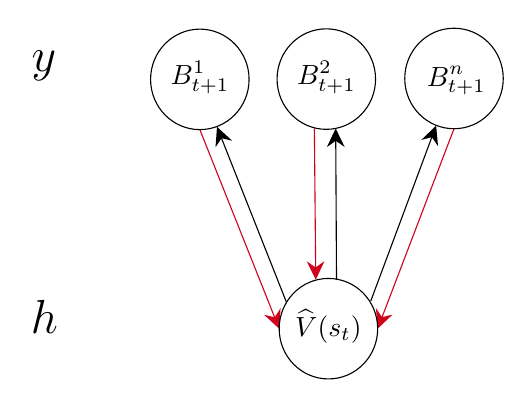
\begin{tikzpicture}[x=0.75pt,y=0.75pt,yscale=-1,xscale=1]
        %uncomment if require: \path (0,300); %set diagram left start at 0, and has height of 300
        
        %Straight Lines [id:da4267952151606098] 
        \draw    (319.82,122) -- (320.2,191.88) ;
        \draw [shift={(319.8,119)}, rotate = 89.69] [fill={rgb, 255:red, 0; green, 0; blue, 0 }  ][line width=0.08]  [draw opacity=0] (8.93,-4.29) -- (0,0) -- (8.93,4.29) -- (5.93,0) -- cycle    ;
        %Straight Lines [id:da6989378371909234] 
        \draw [color={rgb, 255:red, 208; green, 2; blue, 27 }  ,draw opacity=1 ]   (310.17,188.88) -- (309.53,119) ;
        \draw [shift={(310.2,191.88)}, rotate = 269.48] [fill={rgb, 255:red, 208; green, 2; blue, 27 }  ,fill opacity=1 ][line width=0.08]  [draw opacity=0] (8.93,-4.29) -- (0,0) -- (8.93,4.29) -- (5.93,0) -- cycle    ;
        %Shape: Ellipse [id:dp8707618719305075] 
        \draw   (353.08,94.91) .. controls (353.08,81.53) and (363.7,70.7) .. (376.81,70.7) .. controls (389.91,70.7) and (400.53,81.53) .. (400.53,94.91) .. controls (400.53,108.28) and (389.91,119.12) .. (376.81,119.12) .. controls (363.7,119.12) and (353.08,108.28) .. (353.08,94.91) -- cycle ;
        %Straight Lines [id:da13933094112344846] 
        \draw [color={rgb, 255:red, 208; green, 2; blue, 27 }  ,draw opacity=1 ]   (341.1,212.65) -- (376.81,119.12) ;
        \draw [shift={(340.03,215.46)}, rotate = 290.89] [fill={rgb, 255:red, 208; green, 2; blue, 27 }  ,fill opacity=1 ][line width=0.08]  [draw opacity=0] (8.93,-4.29) -- (0,0) -- (8.93,4.29) -- (5.93,0) -- cycle    ;
        %Shape: Ellipse [id:dp9097319337144372] 
        \draw   (291.56,95.2) .. controls (291.56,81.82) and (302.18,70.99) .. (315.29,70.99) .. controls (328.39,70.99) and (339.01,81.82) .. (339.01,95.2) .. controls (339.01,108.57) and (328.39,119.41) .. (315.29,119.41) .. controls (302.18,119.41) and (291.56,108.57) .. (291.56,95.2) -- cycle ;
        %Straight Lines [id:da3769355222150532] 
        \draw [color={rgb, 255:red, 208; green, 2; blue, 27 }  ,draw opacity=1 ]   (291.47,212.67) -- (254.35,119.55) ;
        \draw [shift={(292.58,215.46)}, rotate = 248.27] [fill={rgb, 255:red, 208; green, 2; blue, 27 }  ,fill opacity=1 ][line width=0.08]  [draw opacity=0] (8.93,-4.29) -- (0,0) -- (8.93,4.29) -- (5.93,0) -- cycle    ;
        %Straight Lines [id:da1253267073766362] 
        \draw [color={rgb, 255:red, 0; green, 0; blue, 0 }  ,draw opacity=1 ]   (263.71,120.96) -- (296.02,202.56) ;
        \draw [shift={(262.61,118.17)}, rotate = 68.4] [fill={rgb, 255:red, 0; green, 0; blue, 0 }  ,fill opacity=1 ][line width=0.08]  [draw opacity=0] (8.93,-4.29) -- (0,0) -- (8.93,4.29) -- (5.93,0) -- cycle    ;
        %Shape: Ellipse [id:dp7350394708339132] 
        \draw   (292.58,215.46) .. controls (292.58,202.09) and (303.2,191.25) .. (316.3,191.25) .. controls (329.41,191.25) and (340.03,202.09) .. (340.03,215.46) .. controls (340.03,228.83) and (329.41,239.67) .. (316.3,239.67) .. controls (303.2,239.67) and (292.58,228.83) .. (292.58,215.46) -- cycle ;
        %Shape: Ellipse [id:dp34753658855295044] 
        \draw   (230.62,95.34) .. controls (230.62,81.97) and (241.24,71.13) .. (254.35,71.13) .. controls (267.45,71.13) and (278.07,81.97) .. (278.07,95.34) .. controls (278.07,108.71) and (267.45,119.55) .. (254.35,119.55) .. controls (241.24,119.55) and (230.62,108.71) .. (230.62,95.34) -- cycle ;
        %Straight Lines [id:da6916637423351373] 
        \draw [color={rgb, 255:red, 0; green, 0; blue, 0 }  ,draw opacity=1 ]   (367.15,120.44) -- (336.7,202.13) ;
        \draw [shift={(368.2,117.63)}, rotate = 110.44] [fill={rgb, 255:red, 0; green, 0; blue, 0 }  ,fill opacity=1 ][line width=0.08]  [draw opacity=0] (8.93,-4.29) -- (0,0) -- (8.93,4.29) -- (5.93,0) -- cycle    ;
        
        % Text Node
        \draw (316.33,214.5) node   [align=left] {$\displaystyle \widehat{V}( s_{t})$};
        % Text Node
        \draw (254.43,94.4) node   [align=left] {$\displaystyle B^{1}_{t+1}$};
        % Text Node
        \draw (315.37,94.25) node   [align=left] {$\displaystyle B^{2}_{t+1}$};
        % Text Node
        \draw (377.91,95.99) node   [align=left] {$\displaystyle B^{n}_{t+1}$};
        % Text Node
        \draw (171.67,200.4) node [anchor=north west][inner sep=0.75pt]  [font=\LARGE]  {$h$};
        % Text Node
        \draw (172,80.4) node [anchor=north west][inner sep=0.75pt]  [font=\LARGE]  {$y$};
        
        \end{tikzpicture}
    \end{adjustbox}
\end{center}
\caption{\textbf{Multi-task learning in an ANN}. Adapted from \cite{bengio2017deep}. The figure represents how multi-task learning could be used in an ANN to force the the latent representation $h$ to be a sensible approximation of $V(s_t)$. Here $\widehat{V}(s_t)$ indicates the representation generated by a recurrent layer at time $t$ while $B_{t+1}=\{B^n_{t+1}: n \in N\}$ are $N$ targets quantifying the strength of the next interaction (in terms of frequency and amount of behaviour)  between $I$ and $O$. Black and red arrows are respectively the direction of the computations and the flow of the error gradient. Circles indicate computational blocks similar to those in figures \ref{fig: ffnn} and \ref{fig: ffnn_rnn}.}
\label{fig: multi_task}
\end{figure}
As we mentioned before, in order to generate a latent representation that faithfully approximate the functionality of attributed incentive salience, an ANN should be fitted simultaneously across multiple $O$. This can be achieved through what is known as a global model \cite{wang2019deep} as represented in Figure \ref{fig: global_model}.
\begin{figure}
    \begin{center}
        \begin{adjustbox}{width=0.4\textwidth}

            \tikzset{every picture/.style={line width=0.75pt}} %set default line width to 0.75pt        
            
            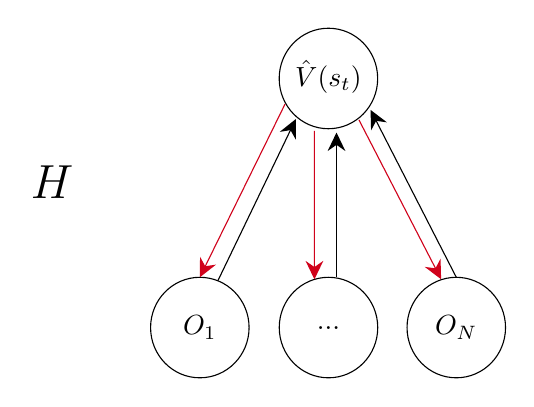
\begin{tikzpicture}[x=0.75pt,y=0.75pt,yscale=-1,xscale=1]
            %uncomment if require: \path (0,488); %set diagram left start at 0, and has height of 488
            
            %Shape: Ellipse [id:dp7350394708339132] 
            \draw   (292.58,215.46) .. controls (292.58,202.09) and (303.2,191.25) .. (316.3,191.25) .. controls (329.41,191.25) and (340.03,202.09) .. (340.03,215.46) .. controls (340.03,228.83) and (329.41,239.67) .. (316.3,239.67) .. controls (303.2,239.67) and (292.58,228.83) .. (292.58,215.46) -- cycle ;
            %Shape: Ellipse [id:dp360084071411103] 
            \draw   (230.62,335.46) .. controls (230.62,322.09) and (241.24,311.25) .. (254.35,311.25) .. controls (267.45,311.25) and (278.07,322.09) .. (278.07,335.46) .. controls (278.07,348.83) and (267.45,359.67) .. (254.35,359.67) .. controls (241.24,359.67) and (230.62,348.83) .. (230.62,335.46) -- cycle ;
            %Shape: Ellipse [id:dp6910252330291001] 
            \draw   (292.61,335.46) .. controls (292.61,322.09) and (303.23,311.25) .. (316.33,311.25) .. controls (329.44,311.25) and (340.06,322.09) .. (340.06,335.46) .. controls (340.06,348.83) and (329.44,359.67) .. (316.33,359.67) .. controls (303.23,359.67) and (292.61,348.83) .. (292.61,335.46) -- cycle ;
            %Shape: Ellipse [id:dp08711921105296772] 
            \draw   (354.18,335.46) .. controls (354.18,322.09) and (364.8,311.25) .. (377.91,311.25) .. controls (391.01,311.25) and (401.63,322.09) .. (401.63,335.46) .. controls (401.63,348.83) and (391.01,359.67) .. (377.91,359.67) .. controls (364.8,359.67) and (354.18,348.83) .. (354.18,335.46) -- cycle ;
            %Straight Lines [id:da1085527921907381] 
            \draw [color={rgb, 255:red, 208; green, 2; blue, 27 }  ,draw opacity=1 ]   (255.67,308.55) -- (295.4,227.8) ;
            \draw [shift={(254.35,311.25)}, rotate = 296.2] [fill={rgb, 255:red, 208; green, 2; blue, 27 }  ,fill opacity=1 ][line width=0.08]  [draw opacity=0] (8.93,-4.29) -- (0,0) -- (8.93,4.29) -- (5.93,0) -- cycle    ;
            %Straight Lines [id:da2379350098727664] 
            \draw [color={rgb, 255:red, 208; green, 2; blue, 27 }  ,draw opacity=1 ]   (309.56,309.25) -- (309.53,240.67) ;
            \draw [shift={(309.56,312.25)}, rotate = 269.98] [fill={rgb, 255:red, 208; green, 2; blue, 27 }  ,fill opacity=1 ][line width=0.08]  [draw opacity=0] (8.93,-4.29) -- (0,0) -- (8.93,4.29) -- (5.93,0) -- cycle    ;
            %Straight Lines [id:da04155200209198706] 
            \draw [color={rgb, 255:red, 0; green, 0; blue, 0 }  ,draw opacity=1 ]   (320.2,244.5) -- (320.2,311) ;
            \draw [shift={(320.2,241.5)}, rotate = 90] [fill={rgb, 255:red, 0; green, 0; blue, 0 }  ,fill opacity=1 ][line width=0.08]  [draw opacity=0] (8.93,-4.29) -- (0,0) -- (8.93,4.29) -- (5.93,0) -- cycle    ;
            %Straight Lines [id:da5357018140104348] 
            \draw [color={rgb, 255:red, 0; green, 0; blue, 0 }  ,draw opacity=1 ]   (299.3,237.7) -- (263,313) ;
            \draw [shift={(300.6,235)}, rotate = 115.74] [fill={rgb, 255:red, 0; green, 0; blue, 0 }  ,fill opacity=1 ][line width=0.08]  [draw opacity=0] (8.93,-4.29) -- (0,0) -- (8.93,4.29) -- (5.93,0) -- cycle    ;
            %Straight Lines [id:da1804092882370092] 
            \draw [color={rgb, 255:red, 208; green, 2; blue, 27 }  ,draw opacity=1 ]   (369.23,309.53) -- (331,235.4) ;
            \draw [shift={(370.6,312.2)}, rotate = 242.72] [fill={rgb, 255:red, 208; green, 2; blue, 27 }  ,fill opacity=1 ][line width=0.08]  [draw opacity=0] (8.93,-4.29) -- (0,0) -- (8.93,4.29) -- (5.93,0) -- cycle    ;
            %Straight Lines [id:da17854416312427956] 
            \draw [color={rgb, 255:red, 0; green, 0; blue, 0 }  ,draw opacity=1 ]   (337.97,233.27) -- (377.91,311.25) ;
            \draw [shift={(336.6,230.6)}, rotate = 62.88] [fill={rgb, 255:red, 0; green, 0; blue, 0 }  ,fill opacity=1 ][line width=0.08]  [draw opacity=0] (8.93,-4.29) -- (0,0) -- (8.93,4.29) -- (5.93,0) -- cycle    ;
            
            % Text Node
            \draw (316.33,214.5) node   [align=left] {$\displaystyle \hat{V}( s_{t})$};
            % Text Node
            \draw (171.67,256.4) node [anchor=north west][inner sep=0.75pt]  [font=\LARGE]  {$H$};
            % Text Node
            \draw (254.35,335.46) node   [align=left] {$\displaystyle O_{1}$};
            % Text Node
            \draw (316.33,335.46) node   [align=left] {$\displaystyle ...$};
            % Text Node
            \draw (377.91,335.46) node   [align=left] {$\displaystyle O_{N}$};
            \end{tikzpicture}
        \end{adjustbox}
    \end{center}
\caption[\textbf{Diagram of a Global Model}]{The figure represents how multiple $O$ can simultaneously contribute to the estimation of $\widehat{V}(s_t)$. Here $\{O_1, \dots, O_N\}$ indicate a set of object on which the ANN is simultaneously fit. Black and red arrows are respectively the direction of the computations and the flow of the error gradient. Circles indicate computational blocks similar to those in figures \ref{fig: ffnn} and \ref{fig: ffnn_rnn}.}
\label{fig: global_model}
\end{figure}
These models can be thought as an extension of mixed effects models \cite{crawley2007mixed} to ANNs and assume that the data on which the model is fitted are drawn from a hierarchy of different populations, each one with its own heterogeneity which can however be brought back to a common single latent factor. The concept is similar to that of Bayesian hierarchical models \cite{gelman2020bayesian} and has the effect of allowing information sharing across the different levels of the hierarchy while also promoting regularization (and therefore generalization)\cite{gelman2020bayesian}. The underlying mechanisms is known as partial pooling \cite{gelman2020bayesian} and can be seen as a middle ground between the over-generalizability of complete pooling (where a single model is estimated across all the levels of the hierarchy) and the over-specificity of un-pooling (where multiple models are estimated, one for each level of the hierarchy). As we can see from Figure \ref{fig: global_model} all the different $O$ contribute to the estimation of a single latent representation $V(s_t)$ which also provide the error gradient for updating their associated parameters.

\subsection{Modelling the contribution of Game Events and Environment Indicators}
\label{modelling_env_and_game_elements}
As we mentioned in chapter \ref{chapter_lit_review}, the current ammount of attributed incentive salience is in part conditioned by the characteristics of the game while its behavioural manifestation can be affected by the environment surrounding the individual. These two factors are not taken into consideration in the modelling framework we just proposed, indeed we assume them to be absorbed, to a certain extent, by the behavioural indicator $B$. If the game characteristics are not able to provide sufficient rewarding experiences or some environmental factors act as an impediment, we can expect to observe less intense and frequent interactions between $I$ and $O$. However in this setting it would be hard to disentangle which factors contributed to the reduction in observed behaviour: was it due to a long-running decline in the level of attributed incentive salience or to an unfavourable conjunction of in-game and out-game events? In this view introducing historical information about the interaction than an individual had with particular characterisitcs of the game object and the environmental context in which they occurred should not just improve the prediction of $\widehat{B}_{t+1}$ but also the estimation of $\widehat{V}(s_t)$. Of course introducing and modelling an extra set of predictors in an ANN is relatively straightforward and increasing the number of available parameters should help incorporating the additional information, however this would make the interpretation of the derived latent representation even more challenging. A possible solution to this problem is to modify the architecture of the ANN in order to integrate the addtional information in a similar way to what Generalized Additive Model (GAM) would do \cite{hastie2017generalized}. Solving the problem of predicting $B_{t+1}$ within a GAM framework for a single game object could have the following formulation:
\begin{gather}
\label{gam}
    \widehat{B}_{t+1} = \beta + f^{B}(B_{t:t-n};\theta^{B}) + f^{G}(G_{t:t-n};\theta^{G}) + f^{Env}(Env_{t:t-n};\theta^{Env})
\end{gather}
here $\beta$ is a generic intercept while $B_{t:t-n}$, $G_{t:t-n}$ and $Env_{t:t-n}$ are temporal series of behavioural metrics, game events and environment indicators up to time $t$. The corresponding functions $f^{B}$, $f^{G}$ and $f^{Env}$ are usually linear or non linear (e.g. splines) additive models. The framework offered by GAM is a good compromise between complexity and explainability as it allows to consider many predictors while enforcing a structural form that makes the function associated to each of them directly interpretable \cite{hastie2017generalized}. In a work by Agarwal et al. \cite{agarwal2021neural} the authors extended the GAM framework to ANN (Neural Addtive Models, NAM), the general idea behind this is to substitute each function expressed in equation \ref{gam} with an appropriated ANN and to derive the prediction of the model as a linear combination of them. The additive nature of NAM, despite posing a constrain on how each function gets integrated with the others, makes it possible to know exactly how each function contribute to the final prediction \cite{hastie2017generalized,agarwal2017quitting}. In our setting we are less interested in retrieving the exact functional form associated to any of the three sources of information (i.e. behaviour, game characteristics and environment) and more in being able to generate separable representations for each one of them. In this view, combining the functional form of equation \ref{gam} with the ideas presented in this chapter we could formulate the estimation of $V(s_t)$ as a non-linear combination of separate functions (all parametrized by ANNs) and subsequently use this for predicting $B_{t+1}$
\begin{gather}
\label{nam}
    \widehat{B_t} = f^{B}(B_{t:t-n}, O;\theta^{B}) \\
    \widehat{G_t} = f^{G}(G_{t:t-n}, O;\theta^{G}) \\ 
    \widehat{Env_t} = f^{Env}(Env_{t:t-n}, O;\theta^{Env}) \\
    \widehat{V}(s_t) = f^{V}(B_t, G_t, Env_t; \theta^{V}) \nonumber
\end{gather}
here $\widehat{B_t}$, $\widehat{G_t}$, $\widehat{Env_t}$ and $\widehat{V}(s_t)$ are representation generated by the respective functions $f$. Each function can be though as being parametrized by a recurrent ANN as specified in section \ref{rnn_theory}. The final representation $\widehat{V}(s_t)$ would then be used for solving the same type of multi-task learning problem presented in section \ref{manifold_learning}. A graphic representation for this can be found in figure \ref{fig: nam_multi_task}.
\begin{figure}
    \begin{center}
        \begin{adjustbox}{width=0.4\textwidth}

            \tikzset{every picture/.style={line width=0.75pt}} %set default line width to 0.75pt        
            
            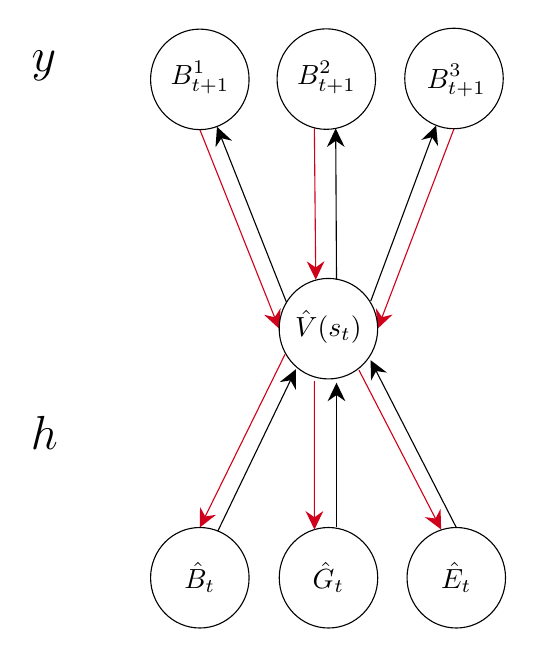
\begin{tikzpicture}[x=0.75pt,y=0.75pt,yscale=-1,xscale=1]
            %uncomment if require: \path (0,488); %set diagram left start at 0, and has height of 488
            
            %Straight Lines [id:da4267952151606098] 
            \draw    (319.82,122) -- (320.2,191.88) ;
            \draw [shift={(319.8,119)}, rotate = 89.69] [fill={rgb, 255:red, 0; green, 0; blue, 0 }  ][line width=0.08]  [draw opacity=0] (8.93,-4.29) -- (0,0) -- (8.93,4.29) -- (5.93,0) -- cycle    ;
            %Straight Lines [id:da6989378371909234] 
            \draw [color={rgb, 255:red, 208; green, 2; blue, 27 }  ,draw opacity=1 ]   (310.17,188.88) -- (309.53,119) ;
            \draw [shift={(310.2,191.88)}, rotate = 269.48] [fill={rgb, 255:red, 208; green, 2; blue, 27 }  ,fill opacity=1 ][line width=0.08]  [draw opacity=0] (8.93,-4.29) -- (0,0) -- (8.93,4.29) -- (5.93,0) -- cycle    ;
            %Shape: Ellipse [id:dp8707618719305075] 
            \draw   (353.08,94.91) .. controls (353.08,81.53) and (363.7,70.7) .. (376.81,70.7) .. controls (389.91,70.7) and (400.53,81.53) .. (400.53,94.91) .. controls (400.53,108.28) and (389.91,119.12) .. (376.81,119.12) .. controls (363.7,119.12) and (353.08,108.28) .. (353.08,94.91) -- cycle ;
            %Straight Lines [id:da13933094112344846] 
            \draw [color={rgb, 255:red, 208; green, 2; blue, 27 }  ,draw opacity=1 ]   (341.1,212.65) -- (376.81,119.12) ;
            \draw [shift={(340.03,215.46)}, rotate = 290.89] [fill={rgb, 255:red, 208; green, 2; blue, 27 }  ,fill opacity=1 ][line width=0.08]  [draw opacity=0] (8.93,-4.29) -- (0,0) -- (8.93,4.29) -- (5.93,0) -- cycle    ;
            %Shape: Ellipse [id:dp9097319337144372] 
            \draw   (291.56,95.2) .. controls (291.56,81.82) and (302.18,70.99) .. (315.29,70.99) .. controls (328.39,70.99) and (339.01,81.82) .. (339.01,95.2) .. controls (339.01,108.57) and (328.39,119.41) .. (315.29,119.41) .. controls (302.18,119.41) and (291.56,108.57) .. (291.56,95.2) -- cycle ;
            %Straight Lines [id:da3769355222150532] 
            \draw [color={rgb, 255:red, 208; green, 2; blue, 27 }  ,draw opacity=1 ]   (291.47,212.67) -- (254.35,119.55) ;
            \draw [shift={(292.58,215.46)}, rotate = 248.27] [fill={rgb, 255:red, 208; green, 2; blue, 27 }  ,fill opacity=1 ][line width=0.08]  [draw opacity=0] (8.93,-4.29) -- (0,0) -- (8.93,4.29) -- (5.93,0) -- cycle    ;
            %Straight Lines [id:da1253267073766362] 
            \draw [color={rgb, 255:red, 0; green, 0; blue, 0 }  ,draw opacity=1 ]   (263.71,120.96) -- (296.02,202.56) ;
            \draw [shift={(262.61,118.17)}, rotate = 68.4] [fill={rgb, 255:red, 0; green, 0; blue, 0 }  ,fill opacity=1 ][line width=0.08]  [draw opacity=0] (8.93,-4.29) -- (0,0) -- (8.93,4.29) -- (5.93,0) -- cycle    ;
            %Shape: Ellipse [id:dp7350394708339132] 
            \draw   (292.58,215.46) .. controls (292.58,202.09) and (303.2,191.25) .. (316.3,191.25) .. controls (329.41,191.25) and (340.03,202.09) .. (340.03,215.46) .. controls (340.03,228.83) and (329.41,239.67) .. (316.3,239.67) .. controls (303.2,239.67) and (292.58,228.83) .. (292.58,215.46) -- cycle ;
            %Shape: Ellipse [id:dp34753658855295044] 
            \draw   (230.62,95.34) .. controls (230.62,81.97) and (241.24,71.13) .. (254.35,71.13) .. controls (267.45,71.13) and (278.07,81.97) .. (278.07,95.34) .. controls (278.07,108.71) and (267.45,119.55) .. (254.35,119.55) .. controls (241.24,119.55) and (230.62,108.71) .. (230.62,95.34) -- cycle ;
            %Straight Lines [id:da6916637423351373] 
            \draw [color={rgb, 255:red, 0; green, 0; blue, 0 }  ,draw opacity=1 ]   (367.15,120.44) -- (336.7,202.13) ;
            \draw [shift={(368.2,117.63)}, rotate = 110.44] [fill={rgb, 255:red, 0; green, 0; blue, 0 }  ,fill opacity=1 ][line width=0.08]  [draw opacity=0] (8.93,-4.29) -- (0,0) -- (8.93,4.29) -- (5.93,0) -- cycle    ;
            %Shape: Ellipse [id:dp360084071411103] 
            \draw   (230.62,335.46) .. controls (230.62,322.09) and (241.24,311.25) .. (254.35,311.25) .. controls (267.45,311.25) and (278.07,322.09) .. (278.07,335.46) .. controls (278.07,348.83) and (267.45,359.67) .. (254.35,359.67) .. controls (241.24,359.67) and (230.62,348.83) .. (230.62,335.46) -- cycle ;
            %Shape: Ellipse [id:dp6910252330291001] 
            \draw   (292.61,335.46) .. controls (292.61,322.09) and (303.23,311.25) .. (316.33,311.25) .. controls (329.44,311.25) and (340.06,322.09) .. (340.06,335.46) .. controls (340.06,348.83) and (329.44,359.67) .. (316.33,359.67) .. controls (303.23,359.67) and (292.61,348.83) .. (292.61,335.46) -- cycle ;
            %Shape: Ellipse [id:dp08711921105296772] 
            \draw   (354.18,335.46) .. controls (354.18,322.09) and (364.8,311.25) .. (377.91,311.25) .. controls (391.01,311.25) and (401.63,322.09) .. (401.63,335.46) .. controls (401.63,348.83) and (391.01,359.67) .. (377.91,359.67) .. controls (364.8,359.67) and (354.18,348.83) .. (354.18,335.46) -- cycle ;
            %Straight Lines [id:da1085527921907381] 
            \draw [color={rgb, 255:red, 208; green, 2; blue, 27 }  ,draw opacity=1 ]   (255.67,308.55) -- (295.4,227.8) ;
            \draw [shift={(254.35,311.25)}, rotate = 296.2] [fill={rgb, 255:red, 208; green, 2; blue, 27 }  ,fill opacity=1 ][line width=0.08]  [draw opacity=0] (8.93,-4.29) -- (0,0) -- (8.93,4.29) -- (5.93,0) -- cycle    ;
            %Straight Lines [id:da2379350098727664] 
            \draw [color={rgb, 255:red, 208; green, 2; blue, 27 }  ,draw opacity=1 ]   (309.56,309.25) -- (309.53,240.67) ;
            \draw [shift={(309.56,312.25)}, rotate = 269.98] [fill={rgb, 255:red, 208; green, 2; blue, 27 }  ,fill opacity=1 ][line width=0.08]  [draw opacity=0] (8.93,-4.29) -- (0,0) -- (8.93,4.29) -- (5.93,0) -- cycle    ;
            %Straight Lines [id:da04155200209198706] 
            \draw [color={rgb, 255:red, 0; green, 0; blue, 0 }  ,draw opacity=1 ]   (320.2,244.5) -- (320.2,311) ;
            \draw [shift={(320.2,241.5)}, rotate = 90] [fill={rgb, 255:red, 0; green, 0; blue, 0 }  ,fill opacity=1 ][line width=0.08]  [draw opacity=0] (8.93,-4.29) -- (0,0) -- (8.93,4.29) -- (5.93,0) -- cycle    ;
            %Straight Lines [id:da5357018140104348] 
            \draw [color={rgb, 255:red, 0; green, 0; blue, 0 }  ,draw opacity=1 ]   (299.3,237.7) -- (263,313) ;
            \draw [shift={(300.6,235)}, rotate = 115.74] [fill={rgb, 255:red, 0; green, 0; blue, 0 }  ,fill opacity=1 ][line width=0.08]  [draw opacity=0] (8.93,-4.29) -- (0,0) -- (8.93,4.29) -- (5.93,0) -- cycle    ;
            %Straight Lines [id:da1804092882370092] 
            \draw [color={rgb, 255:red, 208; green, 2; blue, 27 }  ,draw opacity=1 ]   (369.23,309.53) -- (331,235.4) ;
            \draw [shift={(370.6,312.2)}, rotate = 242.72] [fill={rgb, 255:red, 208; green, 2; blue, 27 }  ,fill opacity=1 ][line width=0.08]  [draw opacity=0] (8.93,-4.29) -- (0,0) -- (8.93,4.29) -- (5.93,0) -- cycle    ;
            %Straight Lines [id:da17854416312427956] 
            \draw [color={rgb, 255:red, 0; green, 0; blue, 0 }  ,draw opacity=1 ]   (337.97,233.27) -- (377.91,311.25) ;
            \draw [shift={(336.6,230.6)}, rotate = 62.88] [fill={rgb, 255:red, 0; green, 0; blue, 0 }  ,fill opacity=1 ][line width=0.08]  [draw opacity=0] (8.93,-4.29) -- (0,0) -- (8.93,4.29) -- (5.93,0) -- cycle    ;
            
            % Text Node
            \draw (316.33,214.5) node   [align=left] {$\displaystyle \hat{V}( s_{t})$};
            % Text Node
            \draw (254.43,94.4) node   [align=left] {$\displaystyle B_{t+1}^{1}$};
            % Text Node
            \draw (315.37,94.25) node   [align=left] {$\displaystyle B_{t+1}^{2}$};
            % Text Node
            \draw (377.91,95.99) node   [align=left] {$\displaystyle B_{t+1}^{3}$};
            % Text Node
            \draw (171.67,256.4) node [anchor=north west][inner sep=0.75pt]  [font=\LARGE]  {$h$};
            % Text Node
            \draw (172,80.4) node [anchor=north west][inner sep=0.75pt]  [font=\LARGE]  {$y$};
            % Text Node
            \draw (254.35,335.46) node   [align=left] {$\displaystyle \hat{B}_{t}$};
            % Text Node
            \draw (316.33,335.46) node   [align=left] {$\displaystyle \hat{G}_{t}$};
            % Text Node
            \draw (377.91,335.46) node   [align=left] {$\displaystyle \hat{E}_{t}$};
            \end{tikzpicture}
        \end{adjustbox}
    \end{center}
\caption{\textbf{Multi-task learning with factorization}. Adapted from \cite{bengio2017deep}. The figure represents how multi-task learning could be extended for distinctly modelling the contribution of different factors in the estimation of $\widehat{V}(s_t)$. Here $\widehat{B_t}$, $\widehat{G_t}$ and $\widehat{E_t}$ indicate the representations generated by 3 distinct recurrent layers taking as input: behavioural, game-events and environmental indicators. The three representations are then parsed by a subsequent recurrent layer producing $\widehat{V}(s_t)$. Similarly to figure \ref{fig: multi_task}, $B_{t+1}=\{B^n_{t+1}: n \in N\}$ are $N$ targets quantifying the strength of the next interaction (in terms of frequency and amount of behaviour)  between $I$ and $O$. Black and red arrows are respectively the direction of the computations and the flow of the error gradient. Circles indicate computational blocks similar to those in figures \ref{fig: ffnn} and \ref{fig: ffnn_rnn}.}
\label{fig: fact_multi_task}
\end{figure}

\section{Discussion}
In this chapter we introduced the idea that latent states, like attributed incentive salience, despite being encoded by high-dimensional signals (e.g. patterns of brain or behavioural activities), can be effectively approximated by a lower dimensional manifold \cite{gallego2017neural, derdikman2011manifold, nieh2021geometry, bromberg2010coding, seung2000manifold, ganmor2015thesaurus, stopfer2003intensity}. We then specified how in the literature the modelling and estimation of attributed incentive salience was carried out through reinforcement learning (i.e. TD learning) \cite{mcclure2003computational,zhang2009neural}. This approach allows to specify the dynamics underlying the process of saliency attribution and offers a direct interpretation of the estimated representations. However, its application in complex naturalistic scenarios can be challenging. Leveraging the knowledge presented in chapter \ref{chapter_lit_review} in combination with insights derived by previous computational model of attributed incentive salience \cite{mcclure2003computational,zhang2009neural} we proposed to approximate the ammount of attributed incentive salience through supervised learning. Due to their reliance on reward mechanics and the ability to provide large volumes of ecologically sound data we thought videogames to be the optimal test bed for our methodology. For this purpose we designed an ANN able to incorporate information about the state of the individual, the environment surrounding them and their interaction with the game. We argued that ANNs with recurrent operations would be well suited for the task as they generate latent representations through dynamical mechanisms that are similar to those of TD learning \cite{barto2004reinforcement}. We also stressed the necessity to learn a single model able to simultaneously incorporate information across multiple videogames in order to obtain representations that obey to the same functional constrains of motivation that we specified in chapter \ref{chapter_lit_review}: namely the ability to simultaneously describe the propensity towards multiple rewarding objects. In the next chapter we will proceeded at illustrating the implementation of the computational model presented in this chapter and the experimental validation of its underlying assumptions.

\chapter{Model Implementation and Testing}
\label{chapter_implementation_testing}
\section{Introduction}
\label{implementation_testing_introduction}

\section{Model Architecture I}
\label{model_architecture_1}
\lorem

\subsection{Data}
To conduct our experiments, we gathered data from six different games published by our partner company, \textit{Square Enix Limited}. Focusing on maintaining heterogeneity in genre and platform, we considered the following titles: \emph{Hitman Go} (hmg), \emph{Hitman Sniper} (hms), \emph{Just Cause 3} (jc3), \emph{Just Cause 4} (jc4), \emph{Life is Strange} (lis), and \emph{Life is Strange: Before the Storm} (lisbf). A general description of each of these titles can be found in Table \ref{gamesdescription}. Data were gathered from any user playing between the game's release and February 2019, allowing us to adopt more robust sampling strategies which utilizes the breadth of virtually the entire user-base. To rule out possible `faulty' but not `naturally abnormal' data, we restricted the data cleaning process to a single filter applied at query time to ignore users having at least one of the considered metric over the game population's \nth{99} percentile. This allowed us to make little assumptions on the distribution of the data as well as providing a convenient stress test for eventual future applications.

\paragraph{Defining the Observation Period}
Because we were interested in estimating survival time and churn probability based only on early user-game interactions it was important to define a cut-off at which point interactions were no longer be considered `early'. We call the period from the user's first interaction till this cut-off the observation period (OP). Choosing the length for the OP was not trivial as there is little indication in the literature about optimal cut-off values. Hence, we decided to visually inspect the data a-priori and extend rules proposed in \cite{drachen2016rapid, milovsevic2017early} to take into account natural inter-individual differences. Therefore, we defined the cut-off as:

\begin{equation}
\label{CutoffOP}
    \text{cutoff} = 
    \Biggl\lceil
        \dfrac
            {min(S_t, S_c)}
            {3}
    \Biggr\rceil
\end{equation}

Where $S_t$ is the total number of game play sessions and $S_c$ is the number of game play sessions before the user completed the game for the first time. In this way we take the first \sfrac{1}{3} of all played sessions for players who churned and the first \sfrac{1}{3} of played sessions before a non-churning player completed the game for the first time. We apply this cut off to the ordered list of all recorded play sessions for a specific user. We decided to use game sessions as the temporal dimension, rather than total minutes played, since we believed it better adjusted for each user's `pace' (i.e. not all the users have the possibility to play at the same frequency). Since the length of the OP has a naturally different distribution between the churning and non-churning population, we stratified our sampling technique to maintain a similar ratio of OP lengths among churners and non churners. This becomes particularly relevant for Experiment 2 and 3 where the length of the OP could leak information in the churn probability estimation task. Summarizing, if a user for example had 9 total sessions recorded, we considered the first 3 for making estimations on what happened after the 9$^{th}$. It goes without saying that at production time the OP is defined only for generating the training samples, the model can be deployed at various stages of previously unseen time series which we simulate in our experiments with the test set. 

\paragraph{Defining the Behavioural Metrics and Targets}
We considered a set of 5 metrics, easily generalizable across games and indicative of behavioural activity, and retrieved them temporally  (i.e. over each game session during the OP), see Table \ref{metricsdescription} for a description. Additionally, we acquired a single context feature specifying the game context from where the metrics were originated. For determining the targets for our survival and churn estimation tasks, we leveraged existing literature on churn prediction \cite{drachen2016rapid, milovsevic2017early, lee2018game, perianez2016churn, runge2014churn, kim2017churn, hadiji2014predicting, xie2015predicting} and survival analysis \cite{viljanen2018playtime, demediuk2018player, lee2018game, bertens2017games}, extending existing rules to accommodate the need to define churn and survival time in single player games with a defined life cycle (i.e. non-GaaS games). We took advantage of having access to the complete session history for all users to create a churn definition which was robust to the variance in play patterns across games, as it takes into account all the recorded inter-session distances. Therefore, the criteria we adopted for defining a user as churner were both: 

\begin{enumerate}
    \item Not completing the game
    \item Being inactive for a period equal or greater to:
        \begin{equation}
            \label{inactivityrule}
            \text{inactivity} = 
            mean(\mathbf{x}) + 2.5 \cdot std(\mathbf{x})
        \end{equation}
\end{enumerate}

For better adjusting for inter-individual differences, we could have applied formula \ref{inactivityrule} to each user individually but this could have created accuracy issue for individuals with very few recorded sessions. Therefore, we opted for a conservative but more robust approach applying inactivity ($\mathbf{x}$) $\forall \mathbf{x} \in X$ where $X$ is the collection of all the considered games and $\mathbf{x}$ is the vector of inter-sessions distances in minutes for a specific game. The use of formula \ref{inactivityrule} allowed us to estimate an inactivity period which was not arbitrarily chosen but statistically defined as ‘extraordinary long’ in accordance with characteristics of play patterns in a particular game. For defining the survival time, we simply computed the total amount of Play Time in minutes for a user minus the amount of Play Time during the OP.

\begin{table}[h] \centering
\caption{\textbf{Considered Metrics over Sessions}}
\label{metricsdescription}
\resizebox{0.5\textwidth}{!}{
\begin{tabular}{@{}ll@{}}
\toprule
\textbf{Metric}            & \textbf{Description}                   \\ \midrule
{Session Time}         & Overall session duration (minutes)              \\ 
{Play Time}            & Session Time spent actively playing (minutes)    \\ 
{Delta Session}        & Temporal distance  between sessions (minutes)   \\ 
{Activity Index}       & Count of user initiated game-play-related actions. E.g.\\ 
                       & `Talk to NPC' or `Acquire Upgrade' were considered valid\\ 
                       & actions while `Click Menu' or `NPC Attacks You' were not.\\
{Activity Diversity}   & Count of unique voluntarily initiated actions \\ 
{Context}              & Name of the game taken into consideration \\ \bottomrule
\end{tabular}
}
\end{table}

\paragraph{Data Preparation}We adopted specific data preparation procedures for each experiment. For the first analysis we collapsed the data over the temporal dimension retrieving mean and standard deviation of each considered features, to this concatenating a one-hot encoded transformation of the context metric. For the second and third experiments we kept the data in the original temporal form. In Experiment 3 only we treated the game context slightly differently, numerically encoding it and separating it from the other feature matrix. Since in Experiment 2 and 3 the length of the OP differed between users, we zero padded each sequence of considered sessions to the length of the longest sequence in the data-set. For each experiment we created a tuning and validation subsets (i.e. 20 and 80 \% of the original data-set) via stratified shuffle split \cite{scikit-learn}, employing the first for hyper-parameters searching and the second for model evaluation.

\subsection{Model Testing Pipeline}
\lorem

\subsection{Results}
\lorem



\section{Model Architecture II}
\label{model_architecture_1}
\lorem

\subsection{Dataset}
\lorem

\subsection{Results}
\lorem

\subsection{Model Testing Pipeline}
\lorem

\section{Model Architecture III}
\label{model_architecture_1}
\lorem

\subsection{Dataset}
\lorem

\subsection{Model Testing Pipeline}
\lorem

\subsection{Results}
\lorem

\chapter{Representation Analysis}
\label{chapter_repr_anal}
\section{Introduction}
\label{representation_analysis_introduction}
In this chapter we will proceed at analyzing the representation generated by the architectures developed in chapter \ref{chapter_implementation_testing}. We will





In this chapter we will present the results of the implementation and validation process used for developing the predictive model described in chapter \ref{chapter_theory_modelling}. Indeed, fundamental to our approach for approximating the latent motivational state of an individual is to have a model able to reliably predict the intensity of future behaviour (i.e. future engagement in a videogame context) given the history of interactions between an individual and a potential rewarding object (i.e. a videogame). To achieve this, we adopted a variation of bottom-up iterative model building \cite{gelman2020bayesian} in which first the simplest version of a model is designed, built and evaluated and then, based on performance and addition theoretical assumptions, a new improved version of the same model is proposed. At each stage of the process we evaluate the new version of the model against alternative approaches in order to test for hypotheses stated in the model design stage. Each section of this chapter corresponds to a different version of the model and will have the following structure. In \textbf{Model Design} we state the task the model is trying to solve, the design of such model and the theoretical assumptions that informed the design. In \textbf{Data} we describe the dataset used for evaluating the performance of our model along with any data-related processing. In \textbf{Model Comparison} we outline the alternative approaches against which the current model is compared and the various procedures and statistical analyses employed. In \textbf{Results} we report the outcomes of the model comparison procedure with particular focus on the assessment of the predictive accuracy. In \textbf{Model Criticism} we discuss what presented in the results section,in light of the theoretical assumptions used when designing the model, and highlight potential improvements to be carried out in the subsequent stage of the model building process. Despite the \textbf{Model Comparison} stage differed slightly between the various stages of the model building process, a common experimental pipeline was adopted. We can see a graphical representation of the latter in Figure \ref{fig: pipeline_eval}
\begin{figure}[h]
  \centering
  \includegraphics[width=\textwidth]{images/chapter_3/pipeline_eval.png}
    \caption[\textbf{Model implementation experimental pipeline}]{Arrows indicate the flow of the pipeline. Big coloured blocks are major pipeline steps, white rectangles indicate sub-tasks within each step.}
    \label{fig: pipeline_eval}
\end{figure}
\begin{figure}[h]
  \centering
  \includegraphics[width=\textwidth]{images/chapter_4/pipeline_inspect.png}
    \caption[\textbf{Model inspection experimental pipeline}]{Arrows indicate the flow of the pipeline. Big coloured blocks are major pipeline steps, white rectangles indicate sub-tasks within each step. This experimental pipeline stems directly from the "Model Evaluation" stage outline in figure \ref{fig: pipeline_eval}.}
    \label{fig: pipeline_inspect}
\end{figure}

\section{Representation Extraction}
\lorem

\subsection{Manifold, Embedding and Neural Networks}
\lorem


\subsection{Dimensionality Reduction and Manifold Approximation}
\label{dim_reduction}
\begin{figure}[h]
  \centering
  \includegraphics[width=\textwidth]{images/chapter_4/ambient.png}
    \caption[\textbf{Swiss rolls in ambient space}]{Swiss rolls in ambient space}
    \label{fig: swiss_ambient}
\end{figure}

\label{dim_reduction}
\begin{figure}[h]
  \centering
  \includegraphics[width=0.8\textwidth]{images/chapter_4/reduced.png}
    \caption[\textbf{PCA and UMAP reduction of Swiss rolls}]{Swiss roles reduced}
    \label{fig: swiss_reduce}
\end{figure}
\lorem

\section{Representation Analysis}
\lorem
After comparing the performance of the RNN model with that of alternative approaches, we proceeded to analyze the representation inferred by the two ANN, with particular attention to the one generated by the RNN. First, we re-fitted both models on a random sample (i.e. 90\%) of the validation-set following the same procedure specified in paragraph \ref{perf_analysis}. Then, we created an encoder composed of all the transformations and relative parameters leading to the shared-representation layer (red highlight in Figure \ref{fig: rnn}). As illustrated in paragraph \ref{manifold_learning}, this is the portion of the model that we expected to approximate the manifold structure of attributed incentive salience. Subsequently, we passed the remaining portion of the validation-set (i.e. 10\%) as an input to the encoders, producing arrays of shape $(batch\times T \times h)$ with $h$ being the number of units in the shared layer and $T$ the number of sessions observed for $batch$ number of individuals. In order to visualize and inspect this multidimensional representation, we used the Uniform Manifold Approximation and Projection (UMAP) algorithm \cite{2018arXivUMAP}, a dimensionality reduction  technique based on manifold learning. Given a high dimensional dataset, UMAP first infers its topological structure and then, using stochastic gradient descent, attempts to structurally reproduce it in a lower dimensional space (two or three for visualization purposes) \cite{2018arXivUMAP}. Compared to other similar dimensionality reduction approaches (for example, the t-distributed Stochastic Neighbor Embedding), UMAP tends to better preserve both global and local structure of the original data, meaning that distances in the underlying dataset should be more faithfully reproduced. Moreover, when given a sequence of datasets with entries related to each other, UMAP is able to maintain these relationships during the optimization process \footnote{See \cite{alignedumap} for implementation details.}. In our case these sequential datasets were the $T$ representations generated by the RNN model after observing $T$ games sessions for a group of individuals. Being able to take into account these temporal relationships allowed us to gather information not just on the characteristics of the representation produced by the RNN model but also on their evolution over time. To clarify, the encoder provided by the ANN was tasked to generate a multidimensional representation where distance represented similarity between individuals with respect to the intensity of their future interactions with a game (see the manifold hypothesis of attributed incentive salience in sections \ref{manifold_state} and \ref{manifold_learning}). The UMAP algorithm made this multidimensional representation interpretable to the human eye approximating it's manifold structure on a 2 dimensional plane 
and allowing us to evaluate the presence of those desirable properties that we mentioned at the beginning of section \ref{method}. Since we did not know the intrinsic dimensionality of the manifold we were trying to approximate, we conducted a Principal Component Analysis (PCA) of the representation generated by the RNN. Despite PCA and UMAP working under radically different assumptions and mechanisms, we thought this could provides us with a lower bound of how much variance we would be able to capture considering only two dimensions. The topological structure of the representation produced by the RNN was inferred by computing the cosine distance in a local neighborhood of 1000 points with a minimum distance of 0.8, while the dimensionality reduction was achieved by running the optimization part of the algorithm for 2000 iterations. The choice of a large neighborhood and minimum distance was made to better capture the global structure of the representation space \footnote{See \cite{umapwebs} for a visualization of the effects of these hyperparameters in UMAP.}.\\
\\
To understand the functions underlying the inferred representation, we conducted an exploratory investigation of the relationship between hidden units' activation in the recurrent layer and predictions produced by the model. To quantify the strength of the observed relationship we employed the Maximal Information Coefficient (MIC) \cite{reshef2011detecting}, a measure of mutual information that can quantify both linear and non-linear association between variables. The MIC can assume values between 0 to 1 with 1 corresponding to a perfect association. We adopted the implementation of UMAP provided McInnes \textit{et. al.} \cite{mcinnes2018umap-software} while the MIC was computed using the python library minepy \cite{albanese2013minerva}. Visualizations were produced using the python libraries matplotlib \cite{hunter2007matplotlib} and seaborn \cite{waskom2021seaborn}.

\subsection{Model Dynamic Prediction}
From figure \ref{pca_emb}A we can observe consistent patterns of cross-correlation for the activity of the artificial neurons constituting the RNN representation. This is supported by the fact that, considering only two dimensions, PCA was able to explain from 30 to 60\% of the variance in the representation generated by the RNN, with maximum explanatory power around 6 and 8 principal components.
\begin{figure}[h]
\centering
\includegraphics[width=0.8\textwidth]{images/chapter_4/pca_repr_42.png}
\caption[\textbf{Hidden units activation analysis of the RNN architecture}]{The activity of the hidden units in the recurrent layer of the RNN architecture showed to be markedly redundant. Panel A shows the cross correlation between the activity of the RNN's artificial neurons in the game object $hms$ going from $t1$ to $t4$. The y and x axes are symmetrical and identifies the RNN artificial neurons while the coloured cells report the Spearman's Rho correlation coefficient for the activation of each pair of neurons. White cells represent combinations for which the correlation coefficient resulted lower than 0.05. \textbf{Two principal components can explain a large portion of variance in the representation generated by the RNN.} Panel B shows the percentage of explained variance by considering 2 to 20 principal components for each game object going from $t1$ to $t4$. The y axis indicates the percentage of explained variance while the x axis the number of principal components considered.}
\label{pca_emb} 
\end{figure}

Inspecting the representation generated by the RNN model at $t1$ (see Figure \ref{full_panel_static}A) we observe that the model was able to effectively distinguish between different game objects while simultaneously encoding for variations in the expected intensity of future interactions. This is illustrated by the fact that each game object occupies different and distinct regions in the representation space while showing a within-object gradient-like organization that places individuals (i.e. single dots) on a continuum based on the estimated magnitude of their future behaviour. This organization is preserved for each of the six targets showing how the representation inferred by the model is a suitable meta-descriptor for different behavioural indicators. As expected, some targets show a very similar but not identical organization (e.g. Future Session Time and Future Session Activity) while others appear to be independent (e.g. Future Session Time and Future Absence). We note that the absolute location of each game aggregate (i.e. all the points belonging to a specific game object) on the 2D plane is arbitrary. As we can see in figures \ref{full_panel_static} and \ref{full_panel_temporal}, this will change at every run of the algorithm due to the stochastic nature of UMAP. Panels \ref{full_panel_static}B and \ref{full_panel_static}C provide more insight into the activation profiles of individual hidden units constituting the generated representation. Panel \ref{full_panel_static}B shows the relationship between the activity of 10 randomly-chosen units and the predictions generated for the five targets. These are essentially transducer functions illustrating how the estimate for a particular target varies (on average) as the output of a units increases or decreases. Each unit seems to encode for multiple non-monotonic functions, one for each of the considered targets. Differences in the shape of these functions reflect similarities between their associated targets. For example, the functions associated to two highly related targets like Future Session Time and Future Session Activity (see panel \ref{full_panel_static}A) appear to be very similar in shape (see panels \ref{full_panel_static}B and \ref{full_panel_static}C). Interestingly, although most units appear to encode for unique functions some of them (e.g. 41 and 44) show an almost identical behaviour. This suggests the presence of redundancy in the functions underlying the representation generated by the RNN model. These observations are clarified in panel \ref{full_panel_static}C, where the functions associated with a single unit (20, indicated by a dark box in \ref{full_panel_static}B) are presented. Here we observe a strong, non-linear relationship between the unit's activity and the estimated targets (see the high MIC values and the line of best fit). In addition, the between-targets variation in MIC values suggest how the chosen unit is not equally informative for all targets.

\begin{figure}[ht]
\centering
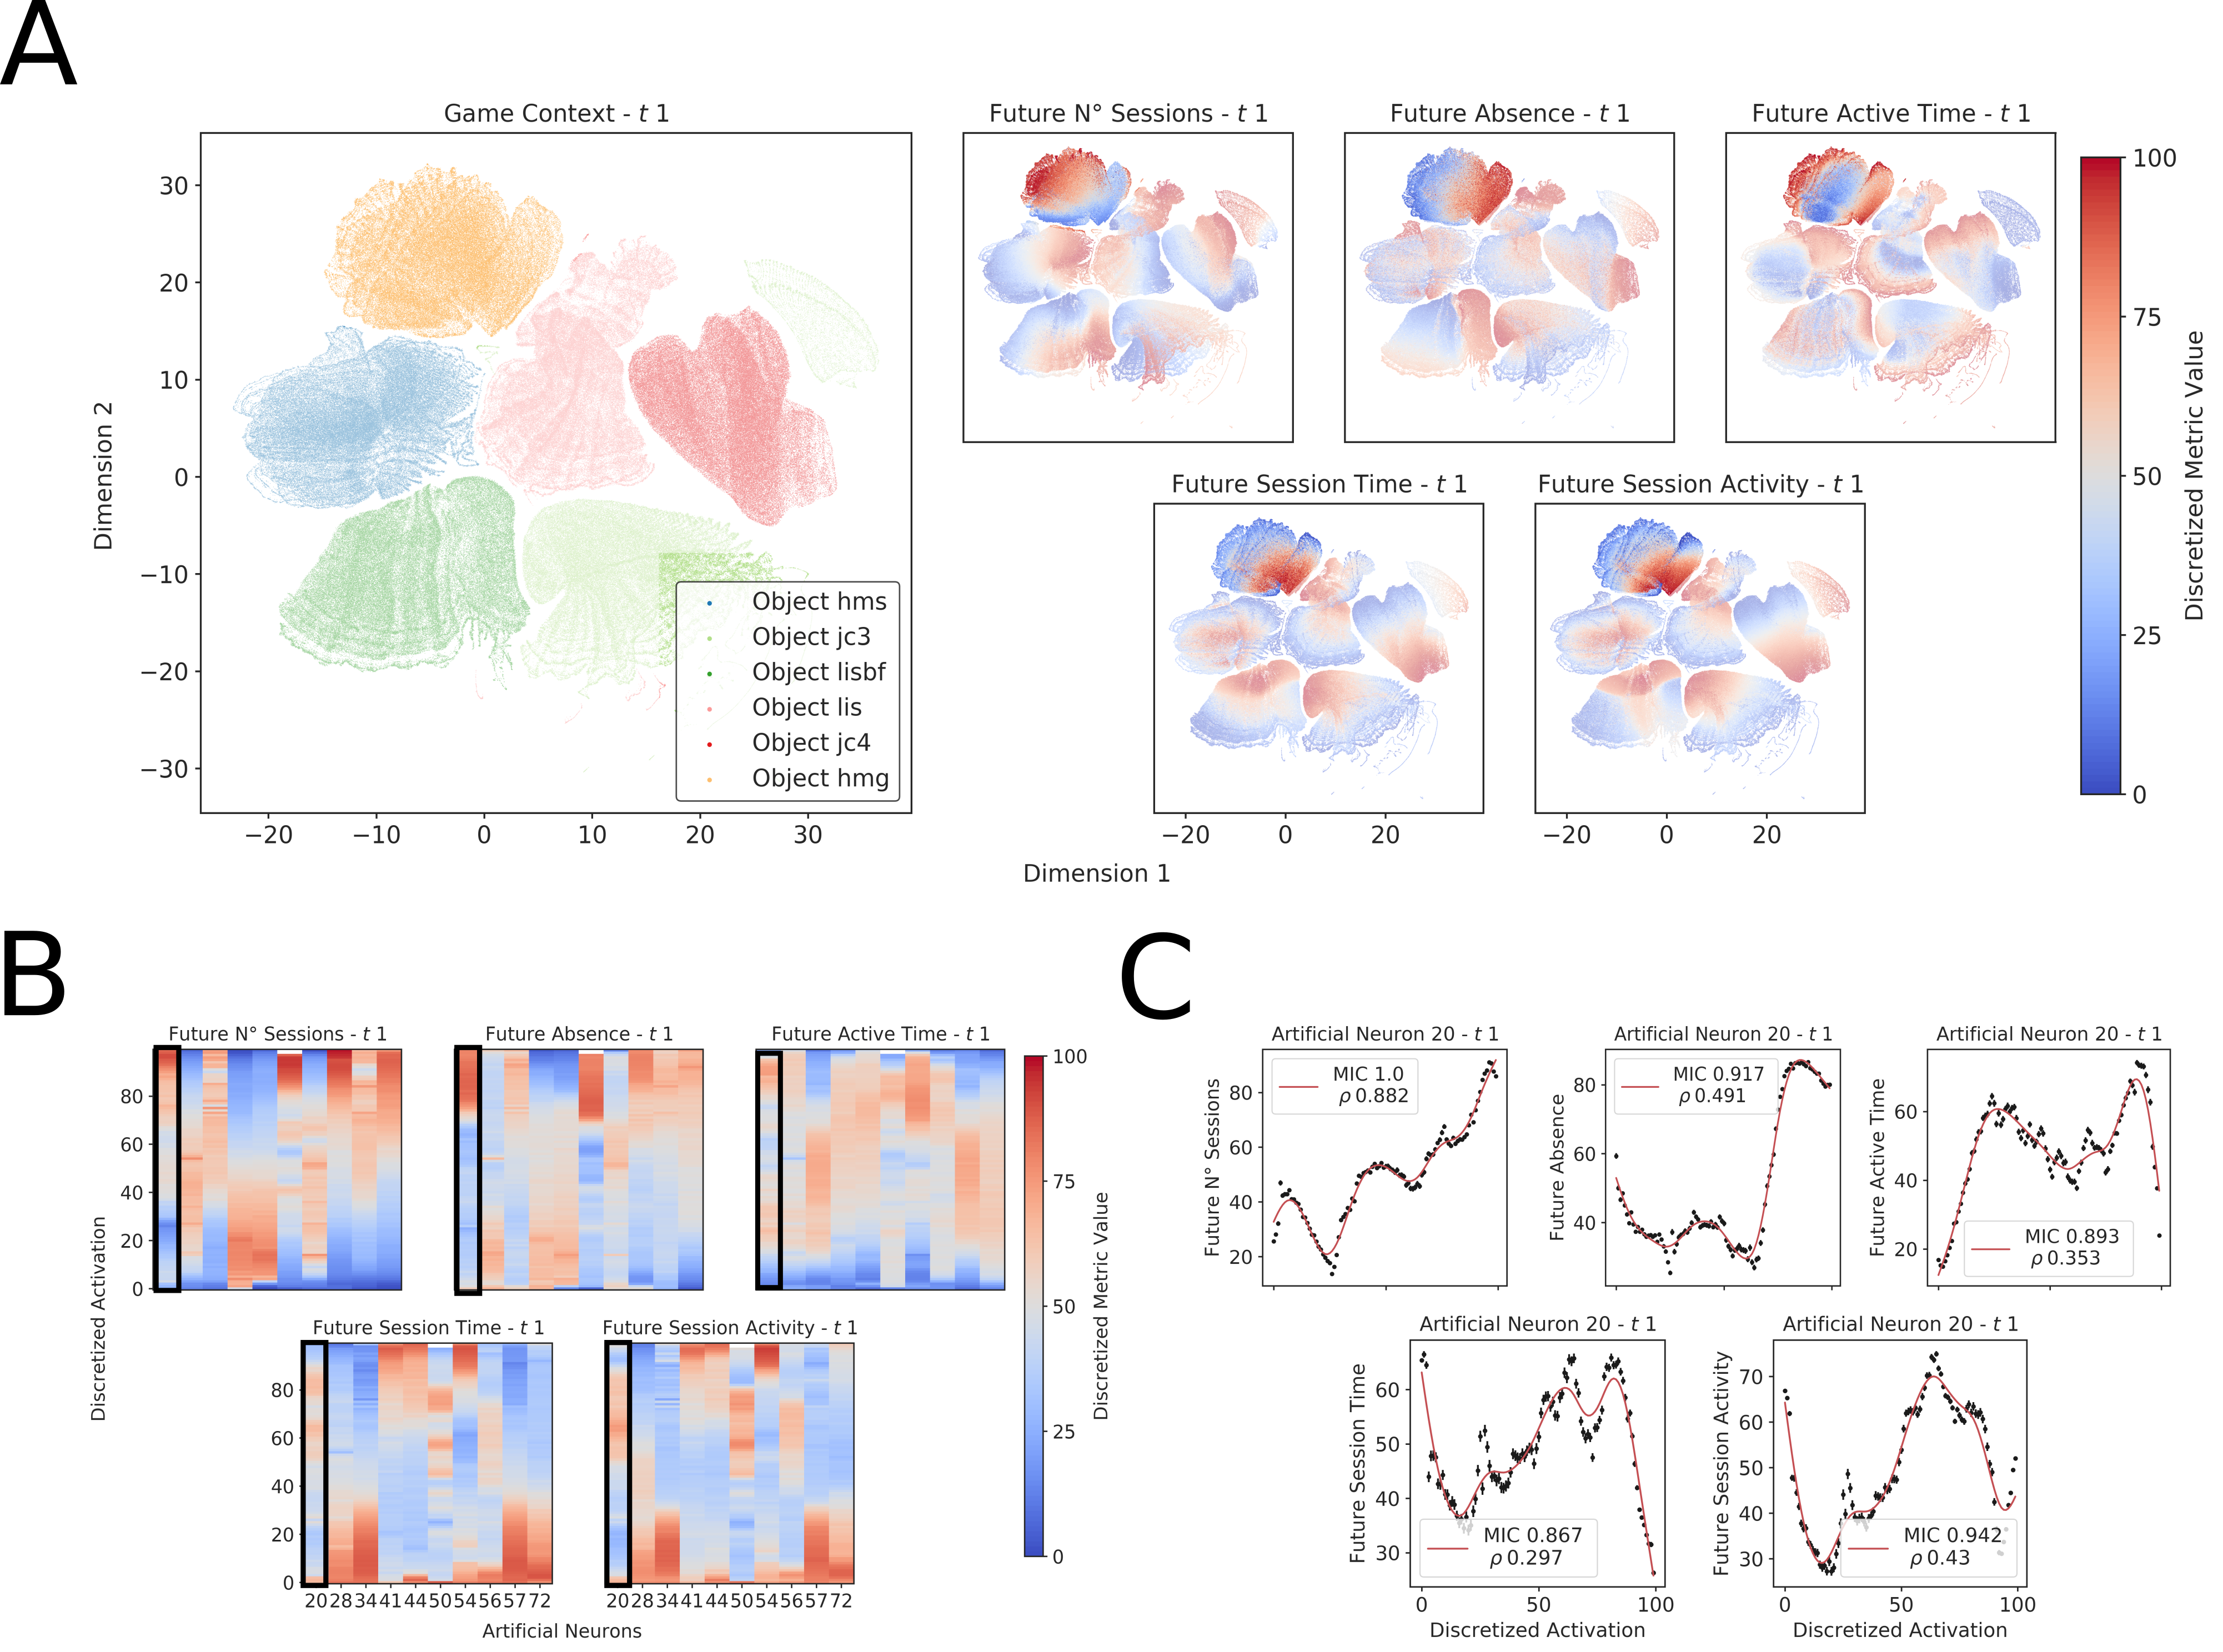
\includegraphics[width=0.9\textwidth]{images/chapter_4/static_repr_42.png}
\caption[\textbf{Lower dimensional representation of the latent state generated by the RNN architecture}]{The representation generated by the RNN model distinguishes between different game objects while maintaining an overarching organization able to capture variations in the expected intensity of future interactions that individuals will have with a specific game object. Panel A shows the two-dimensional projection, produced by UMAP, of the multi-dimensional representation inferred by the RNN at $\mathbf{t1}$ as produced by UMAP. We can read the values of the x and y axes as a coordinate system where proximity represents similarity between points in the original high-dimensional space. Each point indicates the representation inferred by the RNN model after observing one game session from a single user. The colours in the Game Context panel indicate the game object from which the representation is coming. Colours in the small panels represent the discounted sum of all future predictions for a particular target (for example, estimated Future Session Time) $\widehat{B}_{t2:T}$ which is given by $\sum_{i=0}^{t2:T} \gamma^i\widehat{B_i}$ with $\gamma=0.1$ as illustrated in equation \ref{td_v}. \textbf{Each unit  encodes the intensity of future interactions through multiple non-monotonic functions}. Panels B and C show the relationship between the activation of randomly-selected hidden units in the LSTM layer of the RNN and the model's predictions at $\mathbf{t1}$. Panel B shows the relationship between the discretized activation of 10 randomly selected units (artificial neurons) plotted along the y axis and the predictions made by the model at $t1$ (colour coded from blue to red as in the small panels in A) for the game object $hmg$. Panel C shows in more detail the relationship between discretized activation and RNN predictions for a single unit highlighted by a black box in Panel B. Here the x axis indicates the discretized activation while the y axis the mean discretized discounted sum of all future predictions produced by the model. Vertical lines are standard errors of the mean. The red curve is the line of best fit provided by a generalized additive model \cite{serven2018} while the box reports the MIC and the correlation coefficient (Spearman's $\rho$) between the artificial neuron activation and the model's predictions.}
\label{full_panel_static}
\end{figure}
The analyses in Figure \ref{full_panel_static} were performed at a single time point $t1$. When performed at subsequent time points the results appear to be qualitatively similar. For example, focusing on Future Session Time (see Appendix \ref{appendix_representation} for results connected to other targets), we see in Figure \ref{full_panel_temporal}A that the model's ability to segregate different game objects while providing an  overarching representation of the intensity of future interactions is preserved over time. This supports the hypothesis that the representation inferred by our model is dynamic in nature which is further corroborated by panel \ref{full_panel_temporal}D. There we can see how the RNN model was able to individuate a "space" with temporally consistent ”hot” and ”cold” regions between which individuals moved over time depending on the expected intensity of their future interactions. This means that given the history of interaction of a particular individual with a specific game object, our model would determine their "position" (i.e. their "internal state") in the "attributed incentive salience space". This aligns with the manifold hypothesis mentioned in sections \ref{manifold_state} and \ref{manifold_learning}: changes in the propensity to interact with a specific game object (i.e. variations in the amount of attributed incentive salience) can be expressed moving on a manifold embedded within an $h$ dimensional space, with $h$ being the dimensionality of the representation generated by our RNN model. It appears that the hidden units constituting this representation tend to be consistent over time in the type of functions they encode (see Figure \ref{full_panel_temporal}B and C). As expected, we can again observe a strong non linear association between units' activation and targets' predictions, see MIC values and lines of best fit. The decrease in MIC value observed in Figure \ref{full_panel_temporal}C for the artificial neuron 72 might indicate how certain units lose their informative power over time.
\begin{figure}[ht]
\centering
\includegraphics[width=0.8\textwidth]{images/chapter_4/dynamic_repr_42.png}
\caption[\textbf{Lower dimensional representation of the evolution of the latent states generated by the RNN architecture}]{The representation generated by the RNN model appears to maintain its discriminant properties over time. Panel A shows a two-dimensional projection of the multi-dimensional representation inferred by the RNN at $t2$, $t3$ and $t4$. The inferred representation maintains its gradient-like organization over time with an increased ability to differentiate between game objects. As in Figure \ref{full_panel_static}, x and y axes are dimensions individuated by the UMAP algorithm and can be interpreted as a coordinate system where proximity represents similarity between points. Colours in the first row indicate which game object the representation is coming from while those in the second row indicate the discounted sum of future predictions for a single target (i.e. "Future Session Time"). \textbf{The units constituting the generated representation encode for functions that are consistent over time.} Panels B and C show the relationship between units' activation and the model's predictions over time for the game object $hmg$. Different units appear to encode the same target with different non non-monotonic functions which are relatively consistent over time. Panel B illustrates the relationship between the same 10 randomly selected units specified in figure \ref{full_panel_static} and the predictions made by the model for Future Session Time at $t2$, $t3$ and $t4$. Panel C shows in more detail the relationship of the three artificial neurons, highlighted by black boxes in B, across time. Each row is a different unit while each column corresponds to a different $t$. The x axis indicates the discretized activation while the y axis the mean discretized discounted sum of all future predictions. Vertical lines are standard errors of the mean. The red curve is the line of best fit provided by a generalized additive model \cite{serven2018} while the box report the MIC and the correlation coefficient (Spearman's $\rho$) between the artificial neuron activation and the model's predictions. \textbf{The generated representation produces areas of low and high expected intensity among which individuals move over time.} Panel D shows trajectories through time produced by a version of UMAP that incorporates temporal information. Data are drawn from random subsets of individuals having low, medium and high variability in their expected amount of future behaviour. The representation inferred by the RNN model produces "hot" (i.e. the left side) and "cold" (i.e. the right side) regions, representing high and low expected Future Session Time, that are spatially consistent over time. Individuals appear to either stay in the same region or to move between regions over time. Here each line represents variations in the representation generated by the RNN model for a single user over four temporal steps. Continuity is generated by means of cubic spline interpolation for the lines and by linear interpolation for the colours. The x and y axes are the dimensions individuated by the UMAP algorithm while the z axis indicates the associated point in time. Colours indicate the discounted sum of future predictions produced by the model at a specific point in time.}
\label{full_panel_temporal}
\end{figure}

As we mentioned in section \ref{comp_framework}, both ANNs try to predict the intensity of future behaviour given the history of interactions. They do so relying on the same type of metrics, leveraging similar computational mechanisms (i.e. multitask learning and non-linearity) and producing representation according to the same underlying principle (i.e. the manifold hypothesis). Nevertheless, the fact that MLP provides poorer fit to data already suggests that whatever representation it has inferred it is likely a sub-optimal approximation of the manifold structure of incentive salience. Looking at figure \ref{predictive_panel}A, and knowing that UMAP represents differences and similarities between points through distance, we can see how the representation generated by the MLP less clearly differentiate between game objects. On the same figure, we can notice how the gradient representation for the metric Future N° Sessions Time is largely disrupted. This effect is however consistently less pronounced for other metrics (see our \href{https://htmlpreview.github.io/?https://github.com/vb690/approx_incentive_salience/blob/main/notebooks_html/embedding_analysis.html}{GitHub} for additional visualizations), in accordance to the differences we observed in predictive performance (see Figure \ref{model_comp_non_coll}). Recalling what mentioned in section \ref{comp_framework}, the latent state produced by the level of attributed incentive salience should retain at any point in time some predictive power over the intensity of all the future interactions (i.e. not just the one that follows). Figure \ref{rnn_future}B shows the representation generated by RNN and MLP at $t1$ but color coded with the discounted sum of the predictions made from $t4$ onward. We can see that, even if degraded, RNN still preserves some of the desired gradient-like organization which is instead much more disrupted for MLP. This is in accordance to what is shown by Figure \ref{full_panel_temporal}D: the RNN appears to define regions of high and low expected behavioural intensity which are consistent over time rather than constrained to the region around $t+1$.
\begin{figure}[ht]
\centering
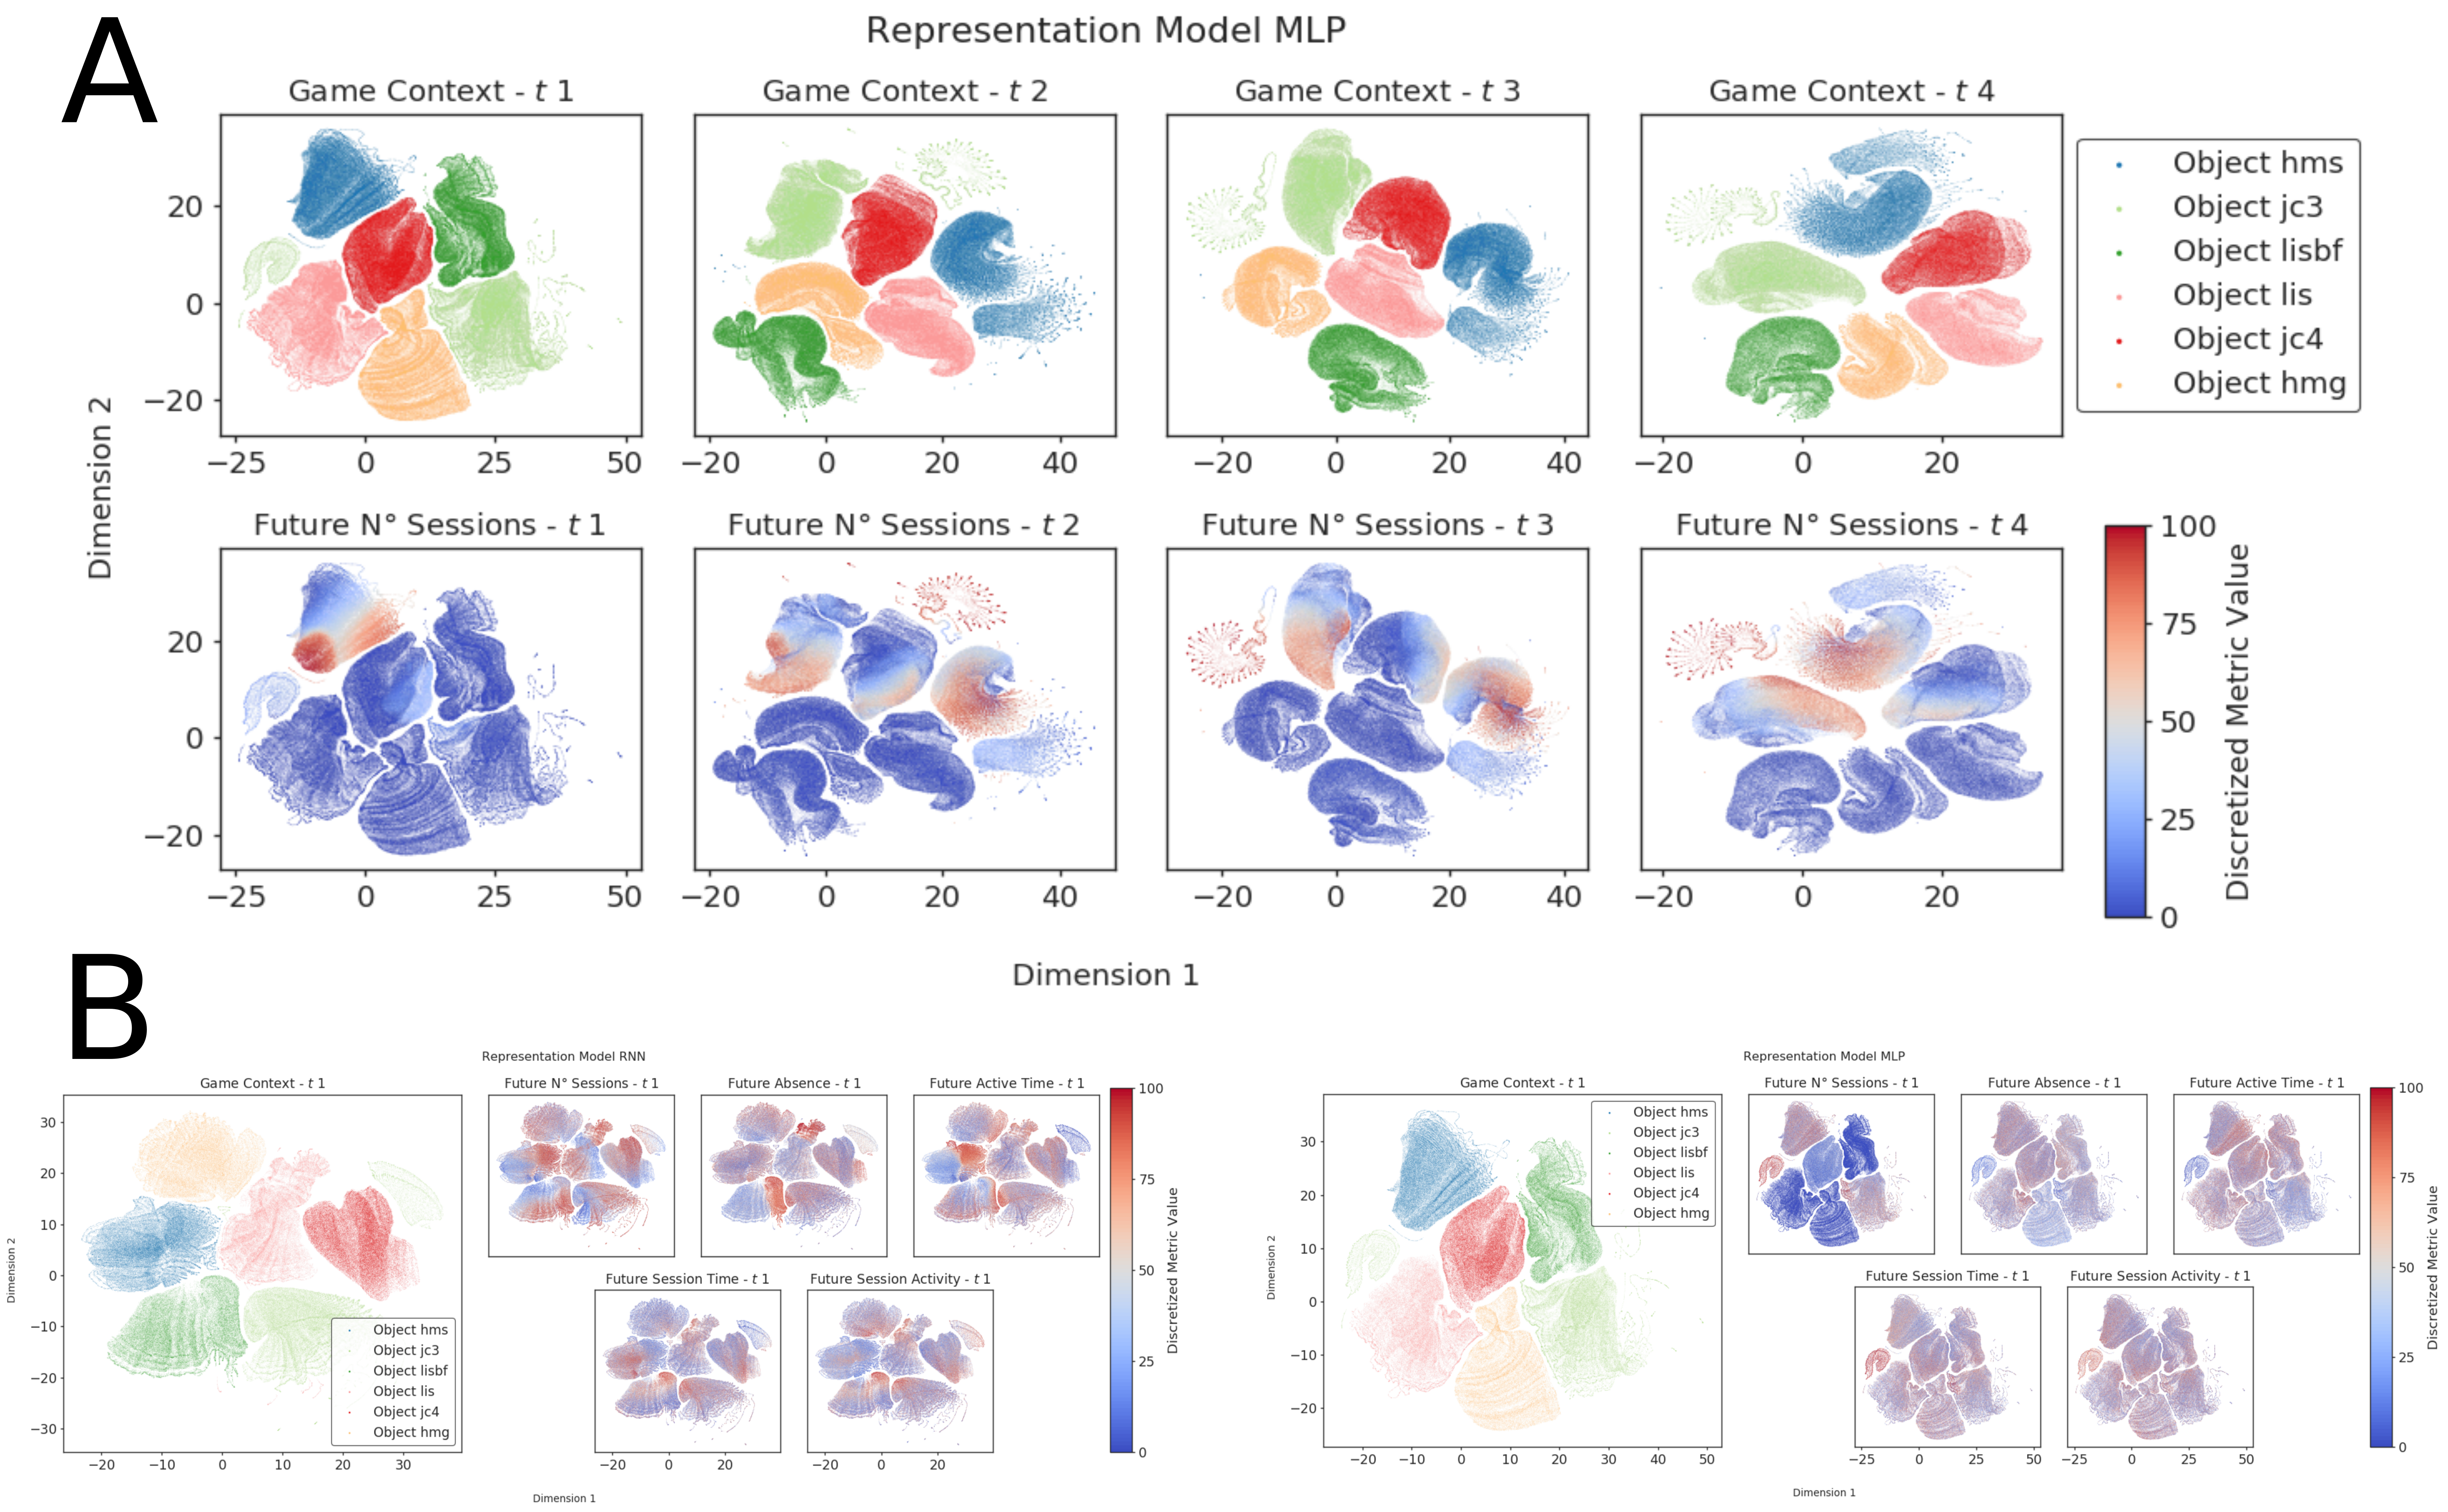
\includegraphics[width=0.9\textwidth]{images/chapter_4/RNN_MLP_repr_42.png}
\caption[\textbf{Lower dimensional representation of the latent states generated by the time-distributed MLP architecture}]{The representation generated by the MLP model is less effective at distinguishing between different game objects and different levels of expected future behaviour intensity. Panel A shows a two-dimensional projection of the multi-dimensional representation inferred by the MLP at $t1$, $t2$, $t3$ and $t4$. Differently from the RNN, the representation shows a disruption in the gradient-like organization and a reduced ability to differentiate between game objects which remain constant over time. The x and y axes are dimensions individuated by the UMAP algorithm and can be interpreted as a coordinate system where proximity represents similarity between points. Colours in the first row indicate which game object the representation is coming from while those in the second row indicate the discounted sum of future predictions for a single target (i.e. "Future N° of Sessions") \textbf{The representation generated by the MLP model is less effective at at distinguishing different levels of expected behaviour intensity for states that are further away in the future.} Panel B shows a two-dimensional projection of the multi-dimensional representation inferred by the RNN (left) and MLP(right) at $t1$ but colour coded with the discounted sum of future predictions from $t4$ onward. The representation generated by the RNN is able to maintain a gradient-like organization even from states that are further away in the future while this capacity is almost entirely lost for the MLP. The colours in the Game Context panel indicate the game object from which the representation is coming. Colours in the small panels represent the discounted sum of all future predictions for a particular target computed from $t4$ onward instead that from $t1$. The x and y axes are the dimensions individuated by the UMAP algorithm.}
\label{predictive_panel}
\end{figure}

\subsection{Model Dynamic Prediction with Covariates}
\lorem

\section{Partition Analysis}
\label{partition_analysese}
We conducted a partition analysis to individuate behavioural profiles associated with the representation generated by our model. As specified in section \ref{manifold_learning} the representation extracted by the encoder at time $t$ can be interpreted as a set of coordinates on the manifold generated by the RNN model after observing $t$ game sessions. Partitioning this representation allows us to identify areas of the manifold that hold information about the history of interactions between an individual and a video game object. These areas may represent variations in the levels of attributed incentive salience and therefore be associated with distinct patterns of behaviour. To partition the data, we used an unsupervised approach applying Mini-Batch K-Means \cite{sculley2010web}, a variation of K-Means, to the representation extracted by the encoder. Given a dataset, the algorithm attempts to divide it by iteratively moving $k$ centroids so as to reduce variance within each partition. The choice of Mini-Batch K-Means was dictated by the fact that it is one of the few distance-based algorithms that scales to very large datasets. To select the optimal $k$ value, we first fitted the algorithm with a varying number of centroids (i.e. 2 to 10) and computed the associated "inertia" (here, a measure of within cluster variance). Since inertia tends to zero as $k$ approaches the number of points in the dataset, we defined the optimal number of partitions as the value of $k$ at which the inertia reached its "elbow" or maximum curvature \cite{satopaa2011finding}. This allows to individuate at which number of partitions there are diminishing returns in terms of within cluster variance reduction. Every instance of Mini-Batch K-Means was initialized 3000 times at random and ran for a maximum of 3000 epochs. The input data were re-scaled to have zero mean and unit-variance and passed to the algorithm in random batches of size $(512 \times h)$. The associated behavioural profiles were found by applying this methodology separately to each game object and retrieving for each partition the mean of all the behavioural metrics over time. The Mini-Batch K-Means implementation used for this analysis was provided by the python library scikit-learn \cite{scikit-learn}. \\
\\
All the analyses were conducted using Python programming language version 3.6.2 \cite{10.5555/1593511}.

\subsection{Model Dynamic Prediction}
\lorem

\subsection{Model Dynamic Prediction with Covariates}
\lorem

\subsection{Discussion}
As mentioned in section  \ref{incentive_salience}, incentive salience attribution produces latent representations of objects which, when imbued with value, make future interactions with those objects more likely and intense \cite{berridge1998role,berridge2004motivation}. The representation generated by our model showed similar functional properties in their global-local organization. At the global level, different game-objects were organized in distinct and coherent regions (see Figure \ref{full_panel_static}A) showing how the model attempted to operate on a meta-level by partitioning a global representation in several object-specific ones. This finding aligns with what highlighted in various work on neural manifold where the responses related to qualitatively different stimuli tends to show a cluster-like organization when reduced to a lower dimensional space \cite{stopfer2003intensity, gallego2017neural, ganmor2015thesaurus}. At the local level, each object-specific representation showed an internal gradient-like organization distinguishing individuals based on the estimated intensity of their future interactions with that specific object. This was true for each of the considered behavioural targets (see Figure \ref{full_panel_static}A) showing how the model attempted to provide an holistic description of the intensity of future interactions. The presence of this type of gradient-like organization emerged in a work by Nieh et al. \cite{nieh2021geometry} when analyzing neural responses during an evidence accumulation task in virtual reality. When reducing the neural activity to a 3 dimensional space, the resulting manifold presented a clear gradient able to code simultaneously for position and levels of accumulated evidence \cite{nieh2021geometry}. A similar finding was present in the work by Stopfner et al. \cite{stopfer2003intensity} where the manifold structure extracted from the activity of olfactory neurons was able to represent qualitative and quantitative differences between odours through a global-local organization similar to that showed in section \ref{repr_results}. The dynamic nature of the representation generated by our approach also nicely fits with that of attributed incentive salience \cite{toates1994comparing,robinson1993neural,zhang2009neural,tindell2009dynamic,berridge2012prediction}. In particular, the fact that the aforementioned global-local organization is maintained over time (see Figure \ref{full_panel_temporal}A) corroborate the hypothesis that our model approximated state changes originated from a dynamic process. In support of this, we also observed that the representation generated by our model was spatially coherent over time: it produced distinct regions of low and high expected intensity between which individuals moved over time (see Figure\ref{full_panel_temporal}D). These results appear to match the definition of motivation and incentive salience attribution specified in section \ref{motivation}: a single overarching process able to dynamically predict the likelyhood and intensity by which individuals will interact with a varied set of objects \cite{simpson2016behavioral,toates1994comparing,berridge2004motivation,zhang2009neural}. Many other cognitive and affective functions might rely on a latent representation that is functionally similar to the one described in our work (e.g. credit assignment and optimal control \cite{wang2018prefrontal, barto2004reinforcement}, cognitive control, learning \cite{skinner1965science} or various forms of reward processing \cite{schultz1997neural, schultz2000reward}). Similarly to attributed incentive salience, these functions are all involved in generating motivated behaviour and heavily rely on reward signals, however none of them is concerned with attributing and describing the motivational saliency that an object possess. This is made evident in the works by McClure et al. \cite{mcclure2003computational} and Zhang et al. \cite{zhang2009neural} where the system involved in salience attribution is functionally separate from the one assigning credit and executing actions: the former provide a representation that informs and biases the decisions taken by the latter serving an almost exclusively qualifying role (see the role of attributed incentive salience in addiction-like conditions \cite{robinson1993neural}). Similarly, the representation generated by our model doesn't provide any insight on the decision making process underlying the observed playing behaviour but simply provide an approximate description of the "motivational pull" that a particular game object has on a particular individual at a certain point in time. The functions encoded by the hidden units constituting the representation appeared to have a series of distinctive properties, namely: redundancy, non linearity, multiplicity (single units code for multiple functions) and consistency over time. These may have played a role in providing the representation generated by our model with its distinctive characteristics. For example, as we mentioned in section \ref{manifold_state} redundancy and inter-correlation are characteristics of the signals from which the manifold representation of internal states arises \cite{seung2000manifold,gallego2017neural}. Multiplicity on the other hand, might be the factor underlying the ability of our model to produce a single unitary representation which holds predictive power over different behavioural targets. Finally, consistency over time could be the mechanisms supporting the type of temporal coherence observed in panel \ref{full_panel_temporal}D. We want to stress that these findings are to be considered exploratory in nature since they do not rely on a-priori hypotheses. A comparison between these computational properties and those underlying the attribution of incentive salience is required and would constitute a potential venue for future investigations. This supports the idea that our approach, by giving full access to its constituent parts, provides a certain degree of interpretability and offers the possibility of generating testable hypotheses. The partition analysis revealed a set of diverse profiles that largely reflect expected behavioural correlates of different levels of attributed incentive salience (i.e. high vs low intensity profiles) \cite{berridge2004motivation}. The various offsets that each partition showed might suggest different levels of predisposition towards the individual game-objects. The dynamic nature of these profiles provided a more granular characterization allowing to observe variations in the entire history of interactions and not just in the expected intensity of future ones. For example, it was possible to see how a higher likelihood of future interactions was supported both by a history of low intensity but high frequency interactions as well as by a series of high frequency and high intensity interactions (see partitions 1 and 2 in Figure\ref{partitioning}B). In this sense, these behavioural profiles can be seen as useful devices for investigating the existence of inter-individual differences in schedules of interactions with potentially rewarding objects.


\chapter{Model Application and Pipeline}
\label{chapter_appliction}
\section{Introduction}
\label{industry_needs}
As we mentioned in chapter \ref{chapter_general_intro}, the aim of this thesis has been twofold: deriving a methodology for inferring the motivational state of individuals while interacting with potentially rewarding object (a videogame in this case) and presenting how this could be used in an applied setting.

In this view, this chapter will focus on sketching the design of a system relying on our methodology for automated engagement prediction. First we will introduce a set of ethical considerations that should be taken into account when designing such system. Subsequently, we will provide an overview on why an industry player (or groups thereof) might need a process for quantifying and predicting engagement and which characteristics this process should have. Finally we will proceed at illustrating a system designed for serving this need, placing particular emphasis on how its components connect with the work presented so far.

\section{Some Ethical Consideration}
\label{ehtical_considerations}
Automated system leveraging behavioural data are now-days used extensively in both low and high stakes scenarios \cite{mehrabi2021survey}, with the potential to have a direct and concrete impact on individuals. For this reason, when designing automated data-driven applications, issues related to fairness should be taken into account. 

By fairness we entail the set of principles and considerations that in recent years are adopted in order to avoid that decisions based on a machine-learned model do not inadvertently bring harm to specific groups of people \cite{mehrabi2021survey}. A complete overview of the issue of fairness in machine learning would be beyond the scope of not just this section but the entire thesis, as it is a vast landscape \cite{mehrabi2021survey} hard to navigate due to its many levels of complexity \cite{corbett2018measure}.  We will therefore focus on two major aspects related to the work presented in this chapter. 

The first aspect concerns biases present in the data on which a machine learning algorithm is fitted. These might be induced by an over or under representation of certain strata of the population that an automated system will ultimately need to serve \cite{mehrabi2021survey}. Given how a large part of machine learning algorithms are fitted to the data (e.g., maximum likelyhood) the risk is that the prediction produced by the algorithm will revert to the mean or in the worst case, will result to be biased with respect to the true characteristics of the population \cite{corbett2018measure, mehrabi2021survey}. Despite the harm that these biases might cause in the context of engagement prediction is not as pronounced as in other areas (e.g., credit, criminal or medical risk assessment), they can still have unexpected repercussion on an individual. 

To this connects the second aspect of fairness that we want to highlight, namely the risk of inadvertently cause harm to individuals which are either temporarily or structurally subject to some form of vulnerability. This might happen as a consequence of automated decision making based on what we call "unconstrained model predictions"


for example if we imagine a system aimed at target high spender users in a game based on gatcha or loot-box mechanics, an unconstrained prediction might inadvertently target individual with a predisposition to or an history of problematic gambling behaviour.

\section{Engagement Quantification and Prediction for the Videogames Industry}
\label{industry_needs}
As we mentioned before despite the industry might be interested in the development of research projects the the focus of this project is less on the advancement of the research field on more focused on the solution of practical problems. 

In this view how does engagement connects with practical problems that the industry has? Very often (if not always) the success of a videogame title is strictly connected with either its ability to retain users or with the experience that users had with the product. The first is pivotal in scenarios where game is treated as a service sold to an audience (similarly to the function of streaming services) while the second is more relevant in scenarios where games are considered digital goods. 

In this context, engagement can be viewed as a measure of how a particular game was, is or will be able to retain users: if an individual is engaged with a particular service it is likely that will keep take advantage of it similarly if an individual had a particular good experience and gladly engaged with a particular digital good it is is more likely that will either suggest it to other users, buy similar products or buy product from the same seller.  

In this view being able to estimate the current propensity of a user towards a specific game translates (in a more or less direct way) to the capacity of assessing if a game is likely to be a success of public and revenue. For this reason it is often the case that videogame publishers and studios try to leverage the information they have available through telemetry system for taking the stock of how a particular game is performing. This is the classical example of analytical reports summarizing various type of game related Key Performance Indicators. 

\section{Multi-context Automated Engagement Prediction and Quantification}
\label{industry_needs}

\section{Data Generation}
\lorem
\subsection{Users}
\lorem
\subsection{Game Contexts}
\lorem

\section{Model Owner}
\lorem
\subsection{Data Storage}
\lorem
\subsection{Model Generation}
\lorem
\paragraph*{Data Generators} \lorem
\paragraph*{Model Configurations} \lorem
\paragraph*{Model Tuning} \lorem
\paragraph*{Model Training} \lorem
\paragraph*{Model Validation} \lorem
\paragraph*{Model Serving} \lorem

\section{Model Consumer}
\lorem
\subsection{Representation Sharing}
\lorem
\subsection{Profile Generation}
\lorem
\subsection{Live Predictions}
\lorem
\subsection{Automated Reporting}
\lorem

\begin{figure}[ht]
\centering
\includegraphics[width=0.7\textwidth]{images/chapter_5/pipeline_diagram.png}
\caption[\textbf{Model Deployment Pipeline}]{The figure represents a simplified system diagram for a potential application of the improved RNN architecture. Solid lines represent low-level components in the system while dashed lines indicate high-level entities. Directional arrows represent the flow of operations inside the system.}
\label{pipeline}
\end{figure}

\chapter{General Discussion}
\label{chapter_general_discussion}
\section{Contributions}

We will now proceed at summarizing the contribution of each chapter in the thesis along with a reflection on its limitations and the potential future research directions that could be taken in order to mitigate them.

\subsection{Chapter 1 - Connecting Motivation and Engagement}
\label{discussion_chapter_one}
In chapter \ref{chapter_lit_review} we focused on providing an overview of the psychological process of motivation highlighting its connection with the construct of engagement.

Relying on the framework proposed by Berridge et al. \cite{berridge1998role} we illustrated how motivation can be seen as process generating latent representations of objects informative of their capacity to produce rewarding experiences. We also illustrated how these representations act as modulatory mechanisms promoting or discouraging future interactions with said objects \cite{berridge2004motivation}.

Through a brief overview of the literature we showed how engagement with digital games can often be described in terms of the cognitive, emotional and behavioural manifestations resulting from the interactions that individuals have with particular game-object \cite{boyle2012engagement, jennett2008measuring, przybylski2010motivational}. These manifestations seem to arise from the interaction between the internal state of the individuals and the structural characteristics of the game \cite{lucas2004sex,o2008user,jennett2008measuring,boyle2012engagement,connolly2012systematic,csikszentmihalyi2014toward}. Moreover, the environment surrounding the individual appears to also have a role in this acting as a modulatory factor \cite{o2008user, bialas2014cultural, vihanga2019weekly, zendle2022transnational}.

Despite various attempts in the literature have been made for connecting these two processes \cite{przybylski2010motivational, nacke2011brainhex, deterding2022mastering}, a clear mechanistic description of this relationship was not always present. In this view, one major contribution of this chapter has been to outline a unifying theoretical framework for understanding the connection between neuroscientific theories of motivation and  two entities. We proposed to see motivation as a latent process arising from the interaction between individuals and (potentially rewarding) objects (i.e., videogames) and to consider engagement as its (noisy) manifestation in the observed behavioural space. 

Relying on this idea, we also highlighted the similarity between data-driven methodology for engagement prediction in a videogame context and latent variable models used in the behavioural neuroscience literature. In particular we showed that if we consider the functional goals a certain motivation-related processes (e.g., incentive salience attribution \cite{berridge2004motivation}) it is possible to understand engagement prediction models as supervise variations of certain latent variables models \cite{luxem2020identifying, mccullough2021unsupervised}.

\subsection{Chapter 2 - From Computational To Supervised Learning Models}
\label{discussion_chapter_two}
In chapter \ref{chapter_theory_modelling} we attempted to translate a computational model used for describing a specific type motivation-related latent process (i.e. attributed incentive salience) into a methodology for approximating such process within a supervised learning context.

The major contribution of this chapter has been to lay out a theoretical framework justifying the use of ANN for generating latent representations that would approximate the construct of attributed incentive salience. In particular, based on existing computational models \cite{mcclure2003computational, zhang2009neural} we illustrated why ANN, and their recurrent variant in particular, would be best suited for the task. We also proposed a series of architectural constrained designed  to encourage an ANN to generate latent representations compliant with the functional characteristics of attributed incentive salience. These were

\begin{enumerate}
    \item The use of a global model architecture for obtaining a single representation able to encompass multiple objects.
    \item The use of multi-task learning in order to force such representation to be a good descriptor of observed behaviour.
    \item The use of GAM-like mechanisms in order to include covariates of interest in the model while maintaining separability and interpretability of the inferred representations.
\end{enumerate}

\subsection{Chapter 3 - Designing, Implementing and Testing the Models }
\label{discussion_chapter_three}
In chapter \ref{chapter_implementation_testing} we proceeded at designing, implementing and testing the ANN architecture presented in chapter \ref{chapter_theory_modelling}.

The contribution of this chapter has been to validate some of the assumptions that were proposed in chapter \ref{chapter_theory_modelling}. We were able to confirm the important role of recurrency and non linearity in generating latent representations with good predictive power. 

\subsection{Chapter 4 - Validating the Properties of the Representations}
\label{discussion_chapter_four}
In comparison to other works focusing on the identification of latent states (or their manifold representation) from behavioural data \cite{calhoun2019unsupervised, luxem2020identifying, pereira2020quantifying, shi2021learning, mccullough2021unsupervised}, the present methodology offers a series of advantages. It does not require the Markov assumption, it generates continuous rather than discrete state space (hence the number of hidden states doesn't need to be specified) and it relies on a more easily scalable class of algorithms. Moreover, in contrast with a general tendency of utilising completely unsupervised techniques for capturing the manifold structure underlying behavioural data \cite{calhoun2019unsupervised, luxem2020identifying, pereira2020quantifying, shi2021learning, mccullough2021unsupervised}, our methodology attempts to extract representations which obey to specific functional constrains (see section \ref{manifold_learning}) and can therefore be more easily interpreted within a specific theoretical framework.

\subsection{Chapter 5 - Illustrating Industrial Applications of the Models}
\label{discussion_chapter_five}

Multi context engegemnt prediction
Multi objective engagement prediction
Dynamic engagement prediction
providing unifying framework for prediction and profiling within the same model.
It generates a representation that can be analyzed (similarly to what has been done in section \ref{representation_analysis}) or provided as input to other algorithms. Indeed, the encoder mentioned in section \ref{representation_analysis} can be thought of as an automatic feature extractor. This can be used to reduce complex time series data of varying length to fixed-size vectors able to describe the propensity of an individual to interact with an object. For example, the analysis presented in section \ref{partition_analysis} showed how this process could be applied for time-series partitioning of large dataset.

The present work leveraged data coming from video games but the adopted approach could easily be applied to other contexts. They only key requirement is the access to behavioural quantifiers describing the amount and intensity of interactions that an individual has with a particular object, service or task. This means that natural areas of application for our approach are those relying on the remote acquisition of behavioural data (e.g. web services or online experiments) but also situations in which large volumes of experimental data are available (e.g. large multi-center studies). 

\section{Conclusion}
In the present work we outlined a methodology for approximating motivation-related latent states in situations where large volumes of behavioural data are available but not direct contact with the individuals that generated them is possible. While doing so we tried to respect computational and theoretical constrains provided by previous works in the field of behavioural and affective neuroscience. 

Indeed we showed that it possible to embed theory-driven knowledge in data-driven approaches, allowing to more easily interpret and test hypotheses on the representation they produce. In comparison to other works focusing on the identification of latent states (or their manifold representation) from behavioural data \citep{calhoun2019unsupervised, luxem2020identifying, pereira2020quantifying, shi2021learning, mccullough2021unsupervised}, our methodology offered a series of advantages. It did not require the Markov assumption, it generated continuous rather than discrete state space and it relied on a more easily scalable class of algorithms. 

Moreover, in contrast with a general tendency of utilising completely unsupervised techniques for capturing the manifold structure underlying behavioural data \citep{calhoun2019unsupervised, luxem2020identifying, pereira2020quantifying, shi2021learning, mccullough2021unsupervised}, our methodology attempted to extract representations which obeyed to specific functional constrains therefore resulted to be more easily interpreted within a specific theoretical framework. In this view, despite our work never aimed at modelling specific cognitive or brain functions, we showed how it is possible to leverage computation model of such functions for designing data-driven methodologies for their inference. This appeared to be important in two fundamental ways. First, it allowed to construct data-driven solutions in a more principled way, rooting their functional form in the nature of the problem they were trying to solve. Second, it made it easier to a-priori specify theory-informed hypotheses and compare them against the behaviour of an otherwise black-box approach.

By connecting this methodology to the construct of engagement we showed how it could be leveraged within an industrial setting as a component of a system designed to perfrom cross-games automated engagement prediction and quantification.

\section{Limitations and Future Directions}
\label{discussion_limitations}
The work we just presented is not exempt from limitations. 

The 

Despite our findings seem to suggest a similarity between the functional characteristics of the representation inferred by our approach and the construct of attributed incentive salience these are the result of mostly qualitative, descriptive or exploratory analyses. 
Since our approach is attempting to solve an inverse problem, the issue of uniqueness arises. Many different latent states might have produced the behavioural patterns that our model observed and there is no guarantee of a strict one-to-one mapping between the representation generated by our model and attributed incentive salience.  More effort should be posed in future research for obtaining a clear formulation of the computations carried out by our architectures. Alternatively, an extensive work of validation could be carried out by comparing the representations generated by our architectures with those generated from data gathered through laboratory or simulation experiments. 

The behavioural profiles individuated in section \ref{partition_analysese} by our partition analyses generally reflect those predicted by theories of reward-driven motivation \citep{thorndike1927law,skinner1965science,berridge2004motivation} but they also show some unexpected and potentially contradictory results. Given the observational setting of our work and the unsupervised approach we adopted, the explanations provided in section \ref{partition_analysese} should be taken with caution and be seen as a method for generating testable hypotheses that should constitute the starting point for future investigations. Indeed, clarifying the the nature of some of the observed discrepancies may require experimental work in more controlled settings. Lastly, despite our approach appeared to deal gracefully with objects having different structural characteristics, these were limited to the domain of video games. In order to verify the generalizability of our approach, future work should include data generated from a variety of contexts (e.g. web services, online and laboratory-based experiments).  



\bibliographystyle{unsrt}
\bibliography{bibliography}

\end{document}

%%%%%%%%%%%%%%%%%%%%%%%%%%%%%%%%%%%%%%%%%%%%%%%%%%%%%%%%%